% -*- coding: utf-8 -*-
%%%%%%%%%%%%%%%%%%%%%%%%%%%%%%%%%%%%%%%%%%%%%%%%%%%%
%%%                                              %%%
%%%     Fichier Maitre pour Jos'Art Books        %%%
%%%        Suivez les instructions ci-apres      %%%
%%%                                              %%%
%%%%%%%%%%%%%%%%%%%%%%%%%%%%%%%%%%%%%%%%%%%%%%%%%%%%
 


%%%%%%%%%      Modele base sur     %%%%%%%%%%%%%%%%%
%%%                                              %%%
%%%     Language Sciences Press MMaster File     %%%
%%%                                              %%%
%%%                                              %%%
%%%%%%%%%%%%%%%%%%%%%%%%%%%%%%%%%%%%%%%%%%%%%%%%%%%%

 
% Everything following a % is ignored
% Some lines start with %. Remove the % to include them

\documentclass[11pt,a4paper,oneside]{book}
  
%%%%%%%%%%%%%%%%%%%%%%%%%%%%%%%%%%%%%%%%%%%%%%%%%%%%
%%%                                              %%%
%%%          additional packages                 %%%
%%%                                              %%%
%%%%%%%%%%%%%%%%%%%%%%%%%%%%%%%%%%%%%%%%%%%%%%%%%%%%

% put all additional commands you need in the 
% following files. If you do not know what this might 
% mean, you can safely ignore this section



%%%%%%%% META DONNEES %%%%%%%%%%%%%%%%%%%%%%
\author{Auteur}
\title{Titre du livre}
\date{}


\input{cfg/pc-packages.tex} 
\input{cfg/pc-cmd.tex}
\input{cfg/pc-env.tex}
\input{cfg/pc-f2sty.tex}

%\bibliography{mabibliographie} 


\begin{document}

	
%%%%%%%%%%%%%%%%%%%%%%%%%%%%%%%%%%%%%%%%%%%%%%%%%%%%
%%%                                              %%%
%%%             Pages liminaires                 %%%
%%%                                              %%%
%%%%%%%%%%%%%%%%%%%%%%%%%%%%%%%%%%%%%%%%%%%%%%%%%%%%
\include{lim/lim_c2c} 

%%%%%%%%%%%%%%%%%%%%%%%%%%%%%%%%%%%%%%%%%%%%%%%%%%%%
%%%                                              %%%
%%%             Frontmatter                      %%%
%%%                                              %%%
%%%%%%%%%%%%%%%%%%%%%%%%%%%%%%%%%%%%%%%%%%%%%%%%%%%%
	

\frontmatter

\tableofcontents
%%%%%%%%%%%%%%%%%%%%%%%%%%%%%%%%%%%%%%%%%%%%%%%%%%%%
%%%                                              %%%
%%%     Fichier Prologue                         %%%
%%%        [Suivez les instructions ci-apres]    %%%
%%%                                              %%%
%%%%%%%%%%%%%%%%%%%%%%%%%%%%%%%%%%%%%%%%%%%%%%%%%%%%

\chapter{Prologue}


Ceci est le prologue
 \lipsum 
%%%%%%%%%%%%%%%%%%%%%%%%%%%%%%%%%%%%%%%%%%%%%%%%%%%%%
%%%                                              %%%
%%%     Fichier Abrev                            %%%
%%%        [Suivez les instructions ci-apres]    %%%
%%%                                              %%%
%%%%%%%%%%%%%%%%%%%%%%%%%%%%%%%%%%%%%%%%%%%%%%%%%%%%

\chapter{Abreviations}

\lipsum[4-7]



%%%%%%%%%%%%%%%%%%%%%%%%%%%%%%%%%%%%%%%%%%%%%%%%%%%%
%%%                                              %%%
%%%             Chapters                         %%%
%%%                                              %%%
%%%%%%%%%%%%%%%%%%%%%%%%%%%%%%%%%%%%%%%%%%%%%%%%%%%%

\mainmatter
% Fichier linf.tex
\ProvidesFile{linf.tex}[version 2018-01-22]
% Decommenter les les lignes avec " %>> " pour tester le fichier
%


	\chapter{Introduction \`a linguistique formelle}
	 
	 \sommaire
	 
	 \section{Introduction}
	  \subsection{Qu'est-ce que la linguistique formelle}
	   La linguistique formelle est une approche de la linguistique qui utilise des outils logico-math�matiques pour analyser les faits de langues et repr�senter les structures langagi�res.
	  \subsection{Utilit� formalisation}
	    Pour comprendre l'utilit� de la formalisation, je vous propose de donner la parole \`a des chercheurs exp�riment�s dans le domaine :
	    
	    \entree{Chomsky 1957, p. 5}
	    \begin{quote}
	    	\motcle{Precisely}  constructed  models for  linguistic  structure  can  play  an  important  role,  both  negative and positive, in the process of discovery itself. By pushing a \motcle{precise} but  inadequate formulation  to an unacceptable conclusion, we can often expose the exact source of this inadequacy and, consequently, gain a deeper understanding of the linguistic data. More positively, a formalized  theory  may automatically  provide solutions for many problems  other  than  those  for  which  it  was  explicitly  designed. [...] I  think  that some of those linguists  who  have  questioned  the  value  of  precise  and  technical development  of linguistic  theory  may  have failed  to  recognize  the productive potential in the method of \motcle{rigorously stating} a proposed theory and applying it strictly to linguistic material with no attempt to avoid  unacceptable  conclusions  by ad hoc adjustments [...].
	    \end{quote}
        \begin{tradcit}
        	Les mod�les linguistiques construits avec \motcle{pr�cision} peuvent jouer un important r�le dans le processus m�me de d�couverte, tant positivement que n�gativement. En proposant une formulation \motcle{pr�cise} \`a une conclusion inacceptable, il est souvent possible d'exposer par la-m�me la source de cette inad�quation et, par cons�\-quent, avoir une meilleure compr�hension des donn�es linguistiques. 
        	Plus important encore, une th�orie formalis�e peut automatiquement fournir des solutions \`a plusieurs probl�mes autres que ceux pour lesquels elle a \'et\'e explicitement con�ue. [...] Je pense que certains des linguistes qui ont remis en cause la valeur des d�veloppements techniques de la th�orie de la linguistique ont peut-�tre manqu� de reconnaitre le potentiel de la m�thode qui consiste \`a \motcle{formuler rigoureusement} une th�orie propos�e et \`a l'appliquer de fa�on stricte au mat�riau linguistique sans vouloir �viter les conclusions inacceptables par des ajustements ad hoc [...].
        \end{tradcit}
	    
	    \entree{Chris Collins, \textit{\#syntactictipoftheday}, Nov. 2017}
	    \begin{quote}
	      I would basically call most of what goes on in generative syntax "semi-formal" (even in semantics). That has been the level of formalization that has allow us to make so many interesting discoveries. But just because the semi-formal mode has been so fruitful, that does not mean there is no place for formalization. 
	      I don't think one should be obsessed by formalization either. That is, just because something is formalized, does not mean it is valuable. But it is a useful tool in certain cases. 	      
	      In other words, the slogan is: Formalization is not a goal in and of itself, but rather a tool to achieve other goals (e.g., making predictions, understanding concepts, etc.). [...] 
	      Formalization is a tool of [...] research, not an end in and of itself.
	    \end{quote}
        \begin{tradcit}
          J'appellerais basiquement la plupart de ce qui se fait en syntaxe g�n�rative "semi-formelle" (m�me en s�mantique). Cela a �t� le niveau de formalisation qui nous a permis de faire autant de d�couvertes inint�ressantes. 
          Mais juste parce que le mode semi-formel a �t� aussi fructueuse, cela ne veut pas dire qu'il n'y a pas de place pour la formalisation. 
          Je ne pense pas non plus qu'il faille �tre obs�d� par la formalisation c'est-\`a-dire que ce n'est pas parce que quelque chose est formalis� que cela a de la valeur. Mais c[la formalisation]'est utile dans certains cas. 
          En d'autres mots,  le slogan est : La formalisation n'est pas un but en soi mais plut�t un outil pour atteindre d'autres buts (e.g., faire des pr�dictions, comprendre des concepts, etc.).
          La formalisation est un outil de recherche, pas une fin en soi.
        \end{tradcit}
        
        \vspace*{1em}
        
        Que faut-il retenir ? La formalisation n'est pas une fin en soi. Juste un outil d'analyse! mais un outil dont il serait dommage de se priver, surtout en tant qu'africain. 
        En effet, la formalisation facilite le traitement automatique des langues. Or, nos langues ont besoin d'�tre automatis�es (e.g., avoir des dictionnaires �lectroniques, des correcteurs orthographiques, des logiciels de reconnaissance vocale, etc.) en vue d'�tre comp�titives. La formalisation est une �tape n\'ecessaire au processus d'automatisation. De toute fa�on, les langages de programmation sont des langages formels.
        
	    \begin{prat}
	      Il y a deux choses qui caract�risent la linguistique formelle, au-del� des symboles math�\-ma\-tiques : la pr�cision et la rigueur jusqu'au bout.
	      \begin{description}
	      	\item[La pr\'ecision: pas de formulations vagues.] Dans une approche formelle, on va  abandonner les formulations \textit{vagues}. e.g., on va pr�f�rer dire 5 cuill�res \`a soupe d'huile, au lieu de ``un peu d'huile".
	      	\item[La rigueur jusqu'au bout.] En linguistique formelle la pr�cision et la rigueur de l'analyse sont au-dessus de la moyenne. Pour faire simple, dans une analyse formelle, on va s'attacher \`a appliquer m�caniquement les proc�dures d�finies.
	      \end{description}
          \entree{\it\bfseries L'usage des variables}
            Les formulations en linguistique formelles font tr�s souvent usage de variables. Les variables sont des lettres de l'alphabet latin (e.g., \textit{x, y, z}) ou grec (e.g., $ \alpha,\ \beta,\ \phi,\ \varphi $), �crites la plupart du temps en minuscule et en italique. Elles peuvent avoir des indices (e.g., $ x_1, y_{23}, z_4 $). Elles peuvent m�me �tre �crites en majuscules. Mais quelque soit la forme sous laquelle elles se pr�sentent, les variables n'ont rien de myst�rieux. Elles sont utilis�es pour indiquer qu'\`a leur place va se trouver quelque chose d'autre. Leur usage est similaire \`a celui ``titre" dans le passage suivant :
            \begin{quote}
            	1.~~ titre\\
            	1.1.~~ titre\\
            	1.1.1.~~ titre
            \end{quote}
	    \end{prat}
	   

    \section{Introduction aux ensembles et aux fonctions}
	  
	  \subsection{Ensembles}
	    \subsubsection{Notion d'ensemble}
	      Un ensemble est simplement un groupe, une collection d'objets -- peu importe leur nature. 
	      Il n'y a pas de restriction sur la nature des objets pouvant constituer un ensemble donn�. Ainsi, un ensemble peut contenir des objets abstraits (e.g., les phon�mes), des objets irr�els (e.g., le pays des singes volants, la plan�te Salybab, la plan�te des singe, le petit prince d'Antoine de Saint-Exup�ry). Il peut aussi arriver que des �l�ments de diverses natures appartiennent � un m�me ensemble.
	      Rien n'interdit d'avoir un ensemble compos� de Homo sapiens, 1, Gerge Cloney, 0, A, a, C, (, �, +, Pluton et La voie lact�e.
	      Il n'y a pas non plus de restriction sur la taille minimale ou maximale d'un ensemble. Un ensemble ne peut pas contenir d'�l�ments du tout -- on l'appelle ensemble vide -- ou, � l'inverse, il peut contenir une infinit� d'�l�ments -- l'ensemble des nombres entiers naturels par exemple.
	      
	      \subsubsection{Diagrammes de Venn}
	        Une fa�on assez amusante de repr�senter les ensembles, c'est de le faire avec des bulles appel�es diagrammes de Venn i.e. ces bulles qu'on voit dans les livres de CP.\\
	        
	        \noindent
	        \begin{demiligne}
	          Ceci est l'ensemble Gbich. Il contient certains des personnages qu'on retrouvent dans ce p�riodique.     
	        \end{demiligne}
            \begin{venndiag}
            	\fbox{\parbox[t]{.45\linewidth}{\hspace{1.5em} Zekinan\hfill\\
            			\hspace*{10.5em} Gazou\hfill\\
            			\hspace*{5.5em} Cauphy\par 
            			\vspace*{.5em} \hfill Tommy\\
            			Jo'Bleck\hfill}}   
            	
            	Ceci est un pseudo-diagramme de Venn	         	
            \end{venndiag}
            
            Les diagrammes de Venn sont assez simples mais peu ad�quats quand il s'agit d'utiliser des fonctionnalit�s les plus inint�ressantes de la th�orie des ensembles -- sans compter qu'il peut �tre fastidieux de les utiliser `dans la vraie vie'. Pensez un peu aux arbres. Il serait plus r�ellement plus fastidieux de manipuler, dans les travaux scientifiques, des diagrammes de Venn que de faire des arbres syntaxiques.
            
            On utilise donc une des notations utilisant des lettres et des symboles. Ainsi, on peut les ins�rer comme pour les transcriptions phon�tiques.  
            
            Nous allons donc introduire \`a partir de maintenant la th�orie des ensembles avec des termes un peu plus formels mais gardez \`a l'esprit qu'il s'agit juste de symboles pour �viter de se compliquer la vie :-).
	        %\cornersize{2}
	        %\ovalbox{\parbox{4cm}{
	         % A\qquad a \quad B \qquad j\\
	          % \hspace{1em} c \quad D \quad e\hfill F\\
	          % f\hspace{2em} g\qquad h 
	        %}}
	      
	      
          \subsubsection{D�crire un ensemble}
	        La th�orie des ensembles est un cadre qui permet de travailler avec des ensembles i.e.  les comparer, voir si les �l�ments de l'un sont en fait les �l�ments d'un autre, construire de nouveaux ensembles \`a partir d'ensembles existants, etc.
	        
	        \noindent Elle repose sur la notion d'appartenance parce que tout ce qu'il faut pour connaitre un ensemble, c'est savoir qui est dedans et qui ne l'est pas -- un peu comme un sac.
	        \begin{notation}
	        	Pour tout objet \textit{a} et tout ensemble \textit{A}, si \textit{a} est dans \textit{A}, on note 
	        	$\bleu{a} \in \bleu{A}$ ; 
	        	et on lit \textit{a} appartient \`a \textit{A} ou $ a $ est un �l�ment de $ A $.
	        \end{notation}
        
	        Il y a donc deux fa�ons de d�crire un ensemble.
	        \begin{notation}[Notation en extension]
		      Pour tout ensemble \bleu{A} qui contient exactement les �l�ments \bleu{a}, \bleu{b}, \bleu{c} et \bleu{d}, on note $ \bleu{A} = \lbrace \bleu{a}, \bleu{b}, \bleu{c}, \bleu{d} \rbrace $\\
	        \end{notation}
	        \begin{e.g.}
		      Ann�e = \{Janvier, F�vrier, Mars, ..., D�cembre\}
	        \end{e.g.} 
	        \begin{rmq}
		      Dans une d�finition en extension d'un ensemble, 
		      \begin{itemize}
			    \item 
			      L'ordre ne compte pas.
			      \begin{e.g.}
				    \{a,b\} = \{b,a\}
				    
			      \end{e.g.}
			    \item 
			      Le nombre d'occurrence d'une unit\'e ne compte pas non plus.
			      \begin{e.g.}
				    \{a,a,a\} = \{a\}
				    
			      \end{e.g.}
		\end{itemize}
	\end{rmq}
    
    \begin{rmq}
      Tous les symboles de relation que nous allons voir admettent un double. Si la relation en question n'a pas cours entre les objets consid�r�s, le symbole sera barr� par un `/'. 
      
      Par exemple si $ a $ n'appartient pas \`a $ A $, on �crira $ a \notin A $ pour dire que $ a $ n'est pas un �l�ment de $ A $. 
    \end{rmq}
	\begin{notation}[Notation en intension]
		Un ensemble \bleu{A} peut �tre �galement not� comme suit : $ \bleu{A} = \lbrace \bleu{x} \, : \, \mbox{crit\`eres \`a remplir pour appartenir \`a } \bleu{A} \rbrace $ $ \bleu{A} = \lbrace \bleu{x} \, \vert \, \mbox{crit\`eres \`a remplir pour appartenir \`a } \bleu{A} \rbrace $ ou .
		On lit \textit{\bleu{A} est l'ensemble des individus \bleu{x} tels que \bleu{x} ...}
	\end{notation}
	
		\ex. Ann�e = \{\textit{x} : \textit{x} est un mois de l'ann�e.\}
	
    
    \begin{appli}
    	Soit X\prim\ le sens de X, �tudiant\prim\ = \{$ x\ \vert\ x $ est un �tudiant\}
    \end{appli}
    \begin{exo}
    	\begin{enumerate}
    	  \item 
    	    D�terminez Ivoirien\prim
    	   \item 
    	     La phrase suivante est-elle vraie ou fausse?
    	     `` Une phrase est un ensemble de mots. " Justifiez votre r�ponse.
    	  \item 
    	    Quand peut-on dire de deux ensembles qu'ils sont �gaux ?
    	  \item  
    	    �crire l'ensemble des entiers naturel plus petits que 2
    	    \begin{enumerate}
    	    	\item[a.] en extension
    	    	\item[b.] en intension
    	    \end{enumerate}
          \item 
            Soit l'ensemble A = \{a,b,4,c\}. Donnez quatre notations en extension de A.
    	\end{enumerate}
    \end{exo}

	\subsubsection{Ensemble d'ensembles}
	Un ensemble peut donc avoir pour �l�ment un autre ensemble.
	  \begin{rmq}
		Si A = \{a, \{b,c\}\} alors b $ \notin $ A.
	  \end{rmq}
      \begin{exo}
      	On donne l'ensemble B = \ens{1, j, \ens{j, 1}, \ens{j,\ens{1, j}, b, 1}}. Combien d'�\-l�\-ments poss�de-t-il ?
      	
      \end{exo}
      \begin{appli}
      	En utilisant la m�thodologie du cours �l�mentaire, analysons la phrase P suivante. P : ``Amlan fait la vaisselle''.
      	
      	\etape\ On sait qu'une phrase est constitu�e d'un groupe sujet (GS) et d'un groupe verbal (GV).
      	
      	Ici GV = fait la vaisselle, GS = Amlan.
      	Donc P = \{Amlan, fait la vaisselle\} 
      	
      	\etape\ Or GV est lui-m�me constitu� de d'un verbe V = \{fait\} et de son compl�ment d'objet direct COD = \{la vaisselle\}.
      	Donc GV = \{fait, la vaisselle\} et \\
      	P = \{Amlan, \{fait, \{la vaisselle\}\}\}
      	
      	\etape\ Il se trouve que le COD aussi est un ensemble constitu� de \textit{la} et \textit{vaisselle}. 
      	
      	Donc \parbox[t]{5cm}{\begin{tabular}{l}
      			COD = \{la, vaisselle\} \\
      			GV = \{fait, \{la, vaisselle\}\} \\
      			P = \{Amlan, \{fait, \{\{la, vaisselle\}\}\}\}
      	\end{tabular}}\par 
      Il y a un probl�me cependant, cette analyse ne nous donne pas la phrase dans sa forme de surface. En effet, les �l�ments sont juste structur�s mais pas ordonn�s. Si P = \{Amlan, \{fait, \{\{la, vaisselle\}\}\}\}, on tout a fait avoir 
      \textit{P : vaisselle la fait Amlan} comme \textit{P : Amlan fait la vaisselle}. 
      
      Nous allons y revenir plus bas, quand nous aurons des outils pour ordonner les ensembles.
      \end{appli}
	\subsubsection{Relations basiques sur les ensembles}
	\paragraph{Inclusion}
	
	\begin{defin}[Inclusion] 
		Quel que soit l'ensemble qu'on consid�re (appelons-le A), il existe un ensemble B dont tous les �l�ments sont aussi des �l�ments de A.
		\\ Cet ensemble est appel� \textit{sous-ensemble de A} ou {\it partie de A}.
		
		On note $ B \subseteq A $ et on lit {\it B est inclus dans A}
	\end{defin}
    
    \paragraph{Inclusion stricte} La relation d'inclusion exige juste que tous les �l�ments de A soient les �l�ments de B sans que n�cessairement les �l�ments de B soient plus nombreux que ceux de A i.e. qu'il existe des �l�ments de B qui ne soient pas �l�ments de A. En clair, A et B peuvent avoir les m�mes �l�ments -- et donc �tre �gaux. L'inclusion stricte exige en plus que les deux ensembles soient diff�rents.
    \begin{defin}[Inclusion stricte] 
      Pour tous ensembles A et B, A est strictement inclus dans B ssi tous les �l�ments de A sont aussi des �l�ments de B et qu'il existe des �l�ments de B qui ne sont pas �l�ments de A.
      \\ $ A $ est appel� \textit{sous-ensemble propre de $ B $}\marginpar{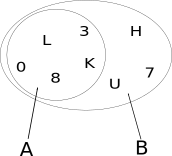
\includegraphics[height=2.1cm,width=1.8cm]{pix/Ainclus-strictB}}.
    	
      On note $ B \subseteq A $ et on lit {\it B est inclus dans A}
    \end{defin}
    \begin{appli}
      La relation d'inclusion stricte est assez appropri\'ee pour mod�liser les concepts d'hyponymie et d'hyperonymie.
      \begin{defin}[Hyponymie]
      	Pour tout mot A et B, A est \textit{hyponyme} de B ssi A\prim\ $ \subset $ B\prim.
      \end{defin}
      \begin{exo}
      	D�finissez la relation d'hyperonymie.
      \end{exo}
    \end{appli}
    
    
    \paragraph{�galit�} Rappelez-vous que deux ensembles sont �gaux ssi ils ont \textit{exactement} les m�mes �l�ments. Formellement, cela nous donne la d�finition suivante. 
    
    \begin{defin}[�galit�]
      Pour deux ensembles quels qu'ils soient -- disons A et B, $ A = B $ ssi $ B \subseteq A $ et $ A \subseteq B $.
    \end{defin}
    
    \begin{exo}
      La phrase suivante est-elle vraie ou fausse : ``Pour tout mots A et B, A et B sont synonymes ssi A\prim\ = B\prim. Justifiez votre r�ponse. 
    \end{exo}

  \subsubsection{Op�rations basiques sur les ensembles}
    \paragraph{Union}
	\begin{defin}[Union]
		Si on consid�re deux ensembles quels qu'ils soient -- disons A et B -- il existe un ensemble C dont les �l�ments sont tous les �l�ments de A et de B -- soit tous �l�ments qui appartiennent ou \`a A ou \`a B. \\ Cet ensemble est appel� \textit{union} de A et B.\marginpar{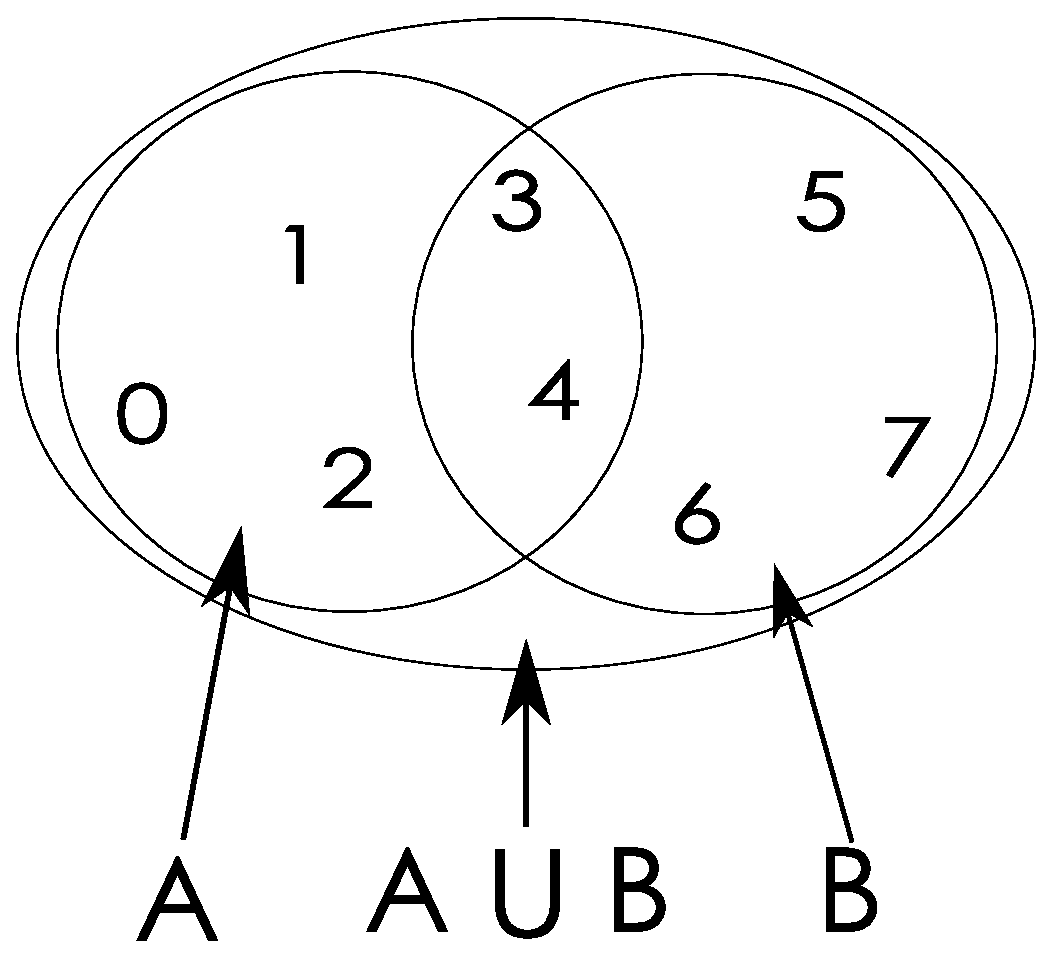
\includegraphics[height=2.1cm,width=1.8cm]{pix/AunionB}}
		
		On note $ C = A \cup B $ et on lit {\it A union B}
	\end{defin}
	
	\paragraph{Intersection}
	\begin{defin}[Intersection]
		Si on consid�re deux ensembles quels qu'ils soient -- disons A et B -- il existe un ensemble C dont les �l�ments sont tous les �l�ments qui appartiennent soit \`a A soit \`a B. \\ Cet ensemble est appel� \textit{intersection} de A et B.\marginpar{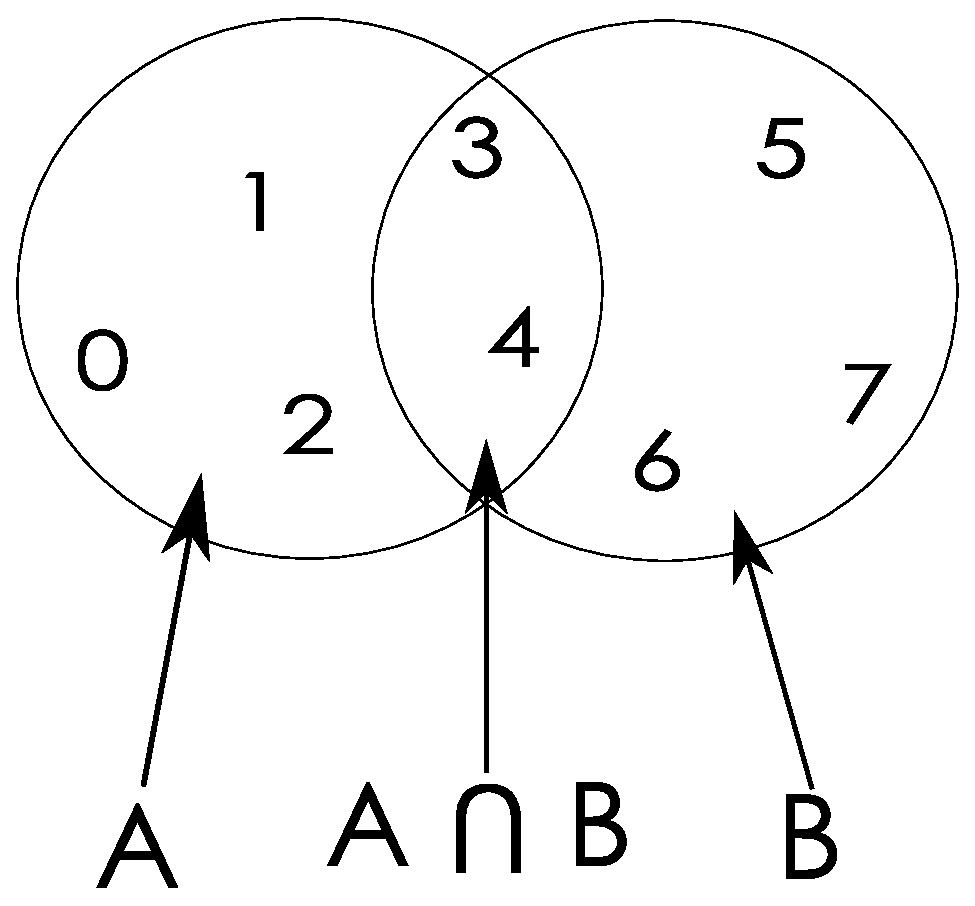
\includegraphics[height=2.1cm,width=1.8cm]{pix/AinterB}}
		
		On note $ C = A \cap B $ et on lit {\it A inter B}
	\end{defin}
	\begin{exo}
	  Donnez une repr�sentation formelle de Etudiant\_ivoirien\prim
	\end{exo}
	\paragraph{Diff�rence}
	  \begin{defin}[Diff�rence d'ensemble]
	    Pour tous ensembles A et B, la diff�rence entre A et B est l'ensemble de tous les �l�ments qui appartiennent \`a A et qui n'appartiennent pas \`a B i.e. \{$ x\ \vert\ x \in A $ et $ x \notin B $\}.\marginpar{$ A \privede B = \{ x\ \vert\ x \in A \mbox{ et } x \notin B \} $} 	
	    
	    On note $ A \privede B $ \couple{et on lit \textit{A priv\'e de B}} ou $ A - B $. 
	  \end{defin}
	   
	  
	  \begin{defin}[Compl�mentaire d'un ensemble]
	     Pour tous ensembles A et B tels que $ A \subset B $, l'ensemble $ C $ tel que $ C = B - A $ est appel� compl�mentaire de A dans B.
	     
	     On note $ C = \complement_AB = B \privede A $.
	     
	     Le compl�mentaire de A peut �tre not� simplement $ \complement A $ ou $ \overline{A} $ ssi B est sp�cifi�.
	  \end{defin}
        
      \begin{exo}
      	Si on se donne un ensemble U de tout ce qui existe dans le monde, auquel on peut doc faire r�f�rence, d�terminez :
      	\begin{enumerate}
      		\item {[--\textsc{anim}]}\prim
      		\item {[--\textsc{x}]}\prim\ pour tous les [+\textsc{x}] tels que [+\textsc{x}]\prim\ est du m�me type que [+\textsc{anim}]\prim\  ou [+\textsc{hum}]\prim\
      	\end{enumerate}
      \end{exo}
	\paragraph{Produit cart�sien et puissance cart�sienne}
	\begin{defin}[Produit cart�sien (de deux ensembles)]\label{def:prod-cart}
		Si on consid�re deux ensembles quels qu'ils soient -- disons A et B -- il existe un ensemble C  qui est l'ensemble des couples dont le premier �l�ment appartient a A et le deuxi�me a B.\\ C est le {produit cart�sien} de A et B.
		
		On note $ C = A \times B $ et on lit {\it A croix B}
		
		On peut aussi �crire $ C = \{\langle a,b\rangle \, \vert \, a \in A \, \mbox{et} \, b \in B\}$
	\end{defin}
	\begin{rmq}
		Dans cet genre d'ensembles, l'ordre compte. $\langle a,b\rangle \neq \langle b,a\rangle $. Aussi A $\times$ B $\neq$ B $\times$ A.
	\end{rmq}
    \begin{exo}
      En vous basant sur la d�finition \ref{def:prod-cart}, proposez une d�finition formelle des concepts de \textit{trait binaire} et \textit{l'ensemble des traits binaires}.
      
    NB: un trait binaire est un trait qui n'admet les valeurs + ou --.
    \end{exo}
    \solut
    \reinit{etap}
    \noindent\etape\ Par d�finition, les traits binaires ont une valeur tir�e d'un ensemble clos \{+, --\} e.g. +\textsc{HAUT}, +N, \textsc{+adv}, etc. On peut donc d�finir un ensemble VALB tel que VALB = \{+,--\}.\\
    
    \noindent\etape\ Dans un trait binaire, on a deux parties le `trait' lui-m�me, et sa valeur. On sait d'o\`u vient la valeur -- de VALB. Il reste \`a d�finir un ensemble qui va contenir tous les `traits'. Mais cet ensemble ne peut �tre en r�alit� l'ensemble des traits puisque +\textsc{trait} est aussi un trait. Il faut donc renommer le symbole qui vient apr�s la valeur e.g. ATR dans +\textsc{ATR}. Appelons-le \textit{attribut}.\\
    
    \noindent\etape\ Il est maintenant possible de d�finir l'ensemble des attributs -- ATT.\\
    
    \noindent\etape\ Puisque de fa�on g�n�ral, dans une trait binaire, la valeur vient avant l'attribut, on a des couples de la forme \couple{valeur,attribut}, l'ensemble des traits T = \{\couple{valeur,attribut} $ \vert\ valeur \in \{+,-\}\mbox{ et } attribut \in ATT $\}  \\
	Or \{\couple{valeur,attribut} $ \vert\ valeur \in \{+,-\}\mbox{ et } attribut \in ATT $\} = VALB $ \times $ ATT\\
	Donc T = VALB $ \times $ ATT.\\
	
	\noindent\etape\ Un trait binaire peut �tre par cons�quent d�fini comme suit : X est un trait binaire ssi $ X \in T $. [cf. e.g. Gazdar et al 1985, Adger 2010 pour des d�finitions similaires]\\
	
	De m�me, on peut construire le produit cart�sien de $ n $ ensembles. Ainsi que le produit cart�sien d'un m�me ensemble $ n $ fois. Dans ce dernier cas, on parle de souvent de \textit{puissance cart�sienne $ n_ieme $} de cet ensemble
	\begin{defin}[Puissance cart�sienne (\textit{n-uplets})]
		Si on consid�re un ensemble quel qu'il soit - disons A - il existe un ensemble B  tel que 
		$ B = \underbrace{A \times A \times ... \times A}_{n \, times} = A^n $\\ 
		Avec $ A^n = \lbrace (x_1, x_2, ..., x_n) \, \vert  \, x_i \in A, 1 
		\leq i 
		\leq n \rbrace $ \\
		
		Les �l�ments d'un tel ensemble sont appel�s {\it n-uplets}. B est appel� \textit{puissance n-i\`eme} de A. \\
	\end{defin} 
	Une autre notation est possible : la notation en {\it forme de mots}.
	\begin{notation}[Notation en forme de mot]
		Si on consid�re un ensemble quel qu'il soit - disons A - il existe un ensemble B  tel que $ B = \underbrace{A \times A \times ... \times A}_{n \, times} = A^n $\\
		Avec $ A^n = \lbrace x_1 \, x_2 \, ...\, x_n \, \vert  \, x_i \in A, 1 
		\leq i \leq n \rbrace $ \\
	\end{notation}
	 
    \begin{appli}
      Soit $ /X/ $ la repr�sentation phonologique du mot X. Comment donner une d�finition g�n�rale de /X/ en utilisant la th�orie des ensembles ? 
      
      \reinit{etap}
      \etape\ On sait que pour tout mot X, /X/ est un ensemble ordonn� de phon�mes. On admet aussi que ces phon�mes sont puis�s dans un stock -- et donc un ensemble qu'on va appeler PH. /X/ peut �tre vu comme un p-uplet form� \`a partir de PH.
      
      \etape\ Il est donc possible d'affirmer ce qui suit Pour X, $ /X/ \in PH^n $ avec $ n $ repr�sentant le nombre de phon�mes qu'il y a dans /X/ [cf. e.g. Kracht]
      
      Il est possible de formuler autrement cette d�finition. En effet, si une th�orie phonologique ne dit que cela, elle ignore un point important : les traits. C'est une th�orie qui assume -- m�me sans le vouloir -- que les phon�mes sont des atomes i.e. des objets qu'on ne peut analyser en �l�ments plus petits. Or, depuis tr�s longtemps d�j� on sait que les phon�mes sont des ensembles de traits. Nous allons donc voir, par une s�rie d'exercices, comment modifier la d�finition que nous venons de donner de /X/. Nous commen�ons par d�finir un phon�me.  
      \begin{exo}
      	En vous appuyant sur la th�orie des ensembles, donnez une d�finition de \textit{phon�me}
      \end{exo}
      
      \solut\reinit{etap}
      \etape\ On se donne  un ensemble de traits phonologiques universel i.e. TPH.
      
      
      \etape\ On remarque qu'un phon�me est tout simplement un sous-ensemble propre de TPH.
      
      \etape\ On donne donc la d�finition suivante : \\
      Pour tout phon�me $ \pi $, \colorbox{lightgray}{$ \pi \subset TPH $.}\par Elle �quivaut \`a celle-ci : 
      Pour tout phon�me $ \pi $, \colorbox{lightgray}{$ \pi \in \wp(TPH) \privede TPH $.} 
          
      \begin{exo}
      	A partir de la d�finition des phon�mes propos�e dans l'exercice pr�c�dent, proposez une d�finition de /X/.
      \end{exo}
  	  
  	  \solut
  	  On d�finit PH. $ PH = \wp(TPH) \privede TPH $. On peut s'arr�ter ici, puisqu'on a r�solu notre probl�me : notre th�orie phonologique sait maintenant que les phon�mes ne sont pas des atomes. La d�finition propos�e au tout d�but est tout \`a fait correcte. il fallait juste ajouter les deux d�finitions : phon�mes et TPH. \par 
  	  N�anmoins, poursuivons notre entreprise de reformulation. Si $ PH = \wp(TPH) \privede TPH $ et que $ /X/ \in PH^n $, alors $ /X/ \in (\wp(TPH) \privede TPH)^n $ [cf. e.g. Collins et Stabler 2016
  	  %\citealt{cs16}
  	  ]
    \end{appli}
	\subsubsection{Relations}
	Il arrive que les �l�ments d'un m�me ensemble, ou d'ensembles diff�rents entretiennent une certaine relation. Par exemple, dans l'exemple \Next, Yao entretient une relation de paternit� avec Aya. 
	\ex.\label{YaoPereAya} Yao est le p�re de Aya
	  
	On dit que la relation de \textit{paternit�} est d�finie \textit{sur} l'ensemble H des humains. De m�me, si on consid�re l'ensemble H des humains et l'ensemble V des voitures, il est facile de se rendre compte qu'il existe des �l�ments de l'ensemble H qui sont en relation de \textit{possession} avec un ou plusieurs �l�ments de l'ensemble V (i.e. certains humains poss�dent une ou plusieurs voitures) On dit alors que la relation de \textit{possession} est une relation \textit{de} H \textit{vers} V. 
	\begin{notation}
		Si \textit{x} entretient avec \textit{y} une relation \textit{R} donn�e, on �crira $\langle x,y\rangle_R$ ou \\ \textit{x R y}.
	\end{notation}
	De fa�on formelle, une relation est un ensemble de couples.
	\begin{defin}[Relation] Soit deux ensembles $A$ et $B$, 
		Si $\mathcal{R}$ est une relation de $A$ vers $B$, alors $\mathcal{R}\subseteq A \times B$.
	\end{defin}
	
	\begin{exo}
	  \newcommand{\amide}[2]{#1 est l'ami de #1}
	  On consid�re la situation suivante :
	  \begin{itemize}
	  	\item \amide{Roland}{Gertrude}
	  	\item \amide{Basile}{Thierry}
	  	\item \amide{Michael}{Martin}
	  	\item \amide{Martin}{Roland}
	  	\item \amide{Marcel}{Marceline}
	  	\item \amide{Julien}{Julienne}
	  \end{itemize}
    Donner le sens de \textit{ami} i.e. ami\prim
	\end{exo}
	
	\begin{exo}
		\newcommand{\amide}[2]{#1 est l'ami de #1}
		On consid�re la situation suivante :
		\begin{itemize}
			\item \amide{Roland}{Gertrude}
			\item \amide{Gertrude}{Marie}
			\item \amide{Marie}{Marceline}
			\item Si \amide{X}{Y} alors \amide{Y}{X}
		\end{itemize}
		\begin{enumerate}
			\item ami\prim = \ens{\couple{Roland, Gertrude}, \couple{Gertrude, Roland}, \couple{Gertrude, Marie}, \couple{Marie, Gertrude}, \couple{Roland, Marie}, \couple{Marie, Marceline}} ?
			\item Sinon donnez l'ensemble correct.
		\end{enumerate}
	\end{exo}
    
    \begin{exo}\label{exo:FrappeMangeChasse}
      \newcommand{\DecRelBin}[3]{#2 #1 #3}
      \newcommand{\DeclarerPersExoFrappeMangeChasse}[7]{
      	\begin{itemize}
      		\item \DecRelBin{frappe}{#1}{#2}
      		\item \DecRelBin{frappe}{#2}{#3}
      		\item \DecRelBin{frappe}{#4}{#5}
      		\item \DecRelBin{mange}{#6}{#7}
      		\item \DecRelBin{chasse}{#6}{#7}
      		\item \DecRelBin{chasse}{#1}{#2}
      		\item \DecRelBin{chasse}{#4}{#5}
      	\end{itemize}
      }
      On consid�re la situation suivante :  \DeclarerPersExoFrappeMangeChasse{Geoffroy}{Wifried}{Marie-Laure}{C\'ecile}{Sophie}{Alexis}{une biche}
      
      D\'eterminez : frapper\prim, manger\prim, chasser\prim, chasser\_et\_manger\prim, chasser\_et\_frapper\prim 
    \end{exo}
	\paragraph{Ensembles ordonn�s et relations d'ordre}
	  Il est possible produire de l'effet d'ordre typique des p-uplets en d�finissant une relation de pr�c�dence (\tprec) sur l'ensemble des �l�ments du p-uplet. Prenons par le mot /pan/. Il poss�de trois �l�ments : a, p, n. Appelons-le M. Donc M = \{p, n, a\}. D�finissons maintenant une relation \tprec\ (i.e. pr�c�de, vient avant) de M vers M telle que \tprec\ = \{\tseq{a,n},\tseq{p,a},\tseq{p,n}\}. On a donc $ a \prec n,\ p\prec a,\ p\prec n $. On peut aussi �crire $ p \prec a \prec n $. Et on obtient un ordre. L'information n\'ecessaire donc pour caract�riser un ensemble ordonn\'e est de savoir qui vient avant qui.\notemar{exemple d'ensemble ordonn\'e : l'ensemble des entiers naturels.}
	  
	  \begin{exo}
	  	Soit $ \mathcal{R} $ une relation de pr�c�dence telle que\\ $ \mathcal{R} = \{\seq{p,a},\seq{p,n},\seq{p,p},\seq{a,p},\seq{a,a},\seq{a,n},\seq{n,a},\seq{n,p}\} $. �crivez le p-uplet �quivalent \`a $ \mathcal{R} $
	  \end{exo}
      
      \begin{exo}
        Donnez l'extension de la relation de pr�c�dence correspondant au p-uplet suivant : \tseq{a,r,n,a,k}
      \end{exo}
      
      \begin{appli}
      	Revenons au probl�me pos\'e par l'analyse de la phrase : les �l�ments �taient juste structur�s mais pas ordonn�s. Une analyse qui assume que P = \{Amlan, \{fait, \{\{la, vaisselle\}\}\}\}, peut aussi bien g�n�rer 
      	\textit{P : vaisselle la fait Amlan} que \textit{P : Amlan fait la vaisselle}. \\
      	La solution \`a ce probl�me nous apparait maintenant �vidente : munir P et ses constituants d'une relation d'ordre.
      	\begin{notation}[Ensemble muni d'une relation]
      	  Si un ensemble E est muni d'une relation $ \mathcal{R} $, on �crit E$_{\mathcal{R}}  $
      	\end{notation}
        Ainsi P = \{Amlan, \{fait, \{\{la, vaisselle\}$_{\mathcal{\prec}}  $ \}$_{\mathcal{\prec}}  $\}$_{\mathcal{\prec}}  $ \}$_{\mathcal{\prec}}  $ soit \chevg\ Amlan, \chevg\ fait, \chevg\chevg\ la, vaisselle\chevd\chevd\chevd\chevd
      \end{appli}
	\subsection{Fonctions}
	
	Une fonction est un type particulier de relations. Seulement, \`a la diff�rence des relations que nous avons d�j� vues, une relation fonctionnelle $-$ ou fonction $-$ est une relation qui est telle que tout �l�ment d'un ensemble donn� (e.g., A) est en relation avec -- ou a pour correspondant -- un et un seul �l�ment d'un (autre) ensemble (e.g., B).
	
	Voici des fonctions qui nous sont famili�res :\marnote{5+2 ne peut donner qu'un seul r�sultat, i.e. 7. De m�me, il n'y a pas deux nombres qui sont double de 3 mais un seul, i.e. 6.}\\
	
	\noindent
	\begin{demiligne}
	  	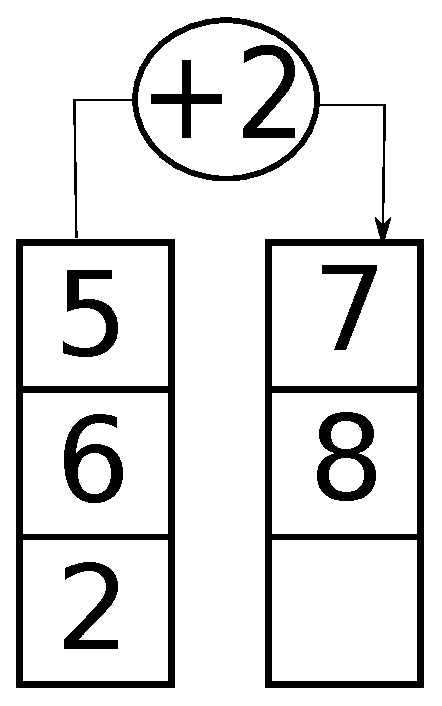
\includegraphics[width=1.8cm,height=2.5cm]{pix/fonctionf}\quad  \parbox[b]{5cm}{ 
	  	Cette fonction fait correspondre \`a tout nombre de la colonne de gauche, le nombre �gal au nombre de d�part ajout\'e de 2.}
	\end{demiligne}
    \begin{demiligne}
    	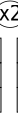
\includegraphics[width=1.8cm,height=2.5cm]{pix/fonctiondouble}\quad \parbox[b]{5cm}{%  
    	Cette fonction fait correspondre \`a tout nombre de la colonne de gauche, le nombre �gal au double du nombre de d�part.}
    \end{demiligne}
    
    Il existe plusieurs fa�ons de noter une fonction. Commen�ons par celle-ci -- probablement la plus famili�re.
    \begin{notation}[Fonction-1]
      Si $ f $ est une fonction qui, a $ x $ associe $ y $, il est possible d'�crire : $ f(x) = y $. On lit : $ f $ de $ x $ est �gal a $ y $.
    \end{notation}
    Par exemple, nos deux fonctions de d�part on dispose de la notation suivante :
    
    \noindent
    \begin{demiligne}
    	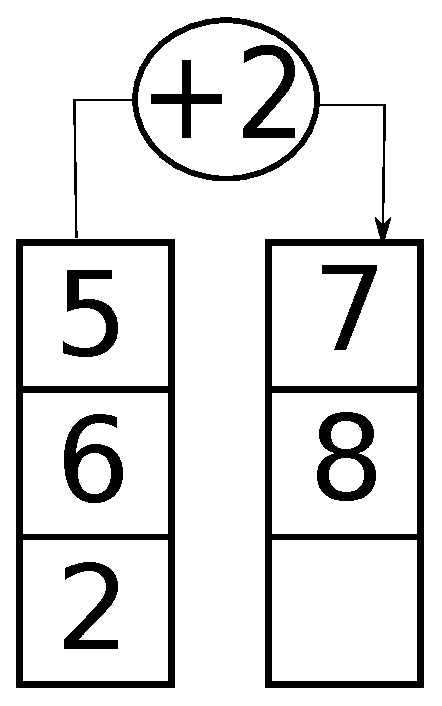
\includegraphics[width=1.8cm,height=2.5cm]{pix/fonctionf}\quad  \parbox[b]{5cm}{ 
    	Si on appelle cette fonction $ A2A $, alors $ A2A(5) = 7 $ et plus g�n�ralement \motcle{$ A2A(x) = x+2 $}}
    	   
    \end{demiligne}
    \begin{demiligne}
    	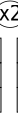
\includegraphics[width=1.8cm,height=2.5cm]{pix/fonctiondouble}\quad \parbox[b]{5cm}{ 
    		Si on appelle cette fonction $ DBL $, alors $ DBL(5) = 10 $ et plus g�n�ralement \motcle{$ A2A(x) = x\times 2 $}}
    \end{demiligne}

	\begin{exo} %
	  On consid\`ere la fonction {\rmfamily\it \bleu{f}} qui \`a chaque �l�ment de l'ensemble {\rmfamily \bleu{A} = \{\bleu{k},\bleu{g},\bleu{b},\bleu{a}\} } associe la majuscule correspondante dans l'ensemble {\rmfamily \bleu{B} =\{\bleu{K},\bleu{G},\bleu{B},\bleu{A}\}}.
	  \begin{enumerate}
	  	\item D�terminez $ MAJ(a) $, $ MAJ(k) $.
	  	\item D�terminez $ MAJ(d) $.
	  	\item Modifiez $ MAJ $ en sorte que seul $ e $ ait une valeur par la fonction. 
	  \end{enumerate}
	  
	\end{exo}

	Il est �galement possible de repr�senter \textit{\bleu{f}} comme suit :
	\begin{center}
		\[%
			f :=
			\left[
			\begin{array}{lll}
				\bleu{a} & \longmapsto & \bleu{A}\\
				\bleu{b} & \longmapsto & \bleu{B}\\
				\bleu{g} & \longmapsto & \bleu{G}\\
				\bleu{k} & \longmapsto & \bleu{K}\\
			\end{array}
			\right]
		\]%
	\end{center}
	
	\begin{termin}[Domaine et co-domaine d'une fonction]\label{term:domaine}
		Soit $ f $ une fonction qui \`a tout \'el\'ement d'un ensemble A associe un seul \'el\'ement d'un ensemble B. A est appel\'e \textit{domaine}, \textit{domaine de d\'efinition} ou encore \textit{ensemble de d\'efinition} de $ f $. B est appel\'e \textit{co-domaine} de $ f $.\\
	\end{termin}
	\begin{notation}
		Soit $ f $ une fonction ayant pour domaine A et pour co-domaine B, on \'ecrit : $ f : A \rightarrow B $ ; et on lit $ f $ est une fonction de $ A $ vers $ B $.
	\end{notation}

	\begin{prat}[Les r�gles comme fonctions]
	  Supposons une langue o\`u tous les phon�mes sourds deviennent sonore quand ils sont pr�c�d�s d'un segment sonores. Sch�matiquement, on a ce qui suit :
	  \[
	    C_{[\textsc{-son}]} \rightarrow C_{[\textsc{+son}]} / \_[\textsc{+son}]
	  \]
	  Cette r�gle peut �tre mod�lis�e comme une fonction qui change tout phon�me sourd en phon�me sonore lorsqu'il pr�c�de imm�diatement un segment poss�dant un trait [\textsc{+son}]. Nous allons proc�der par �tape.
	  
	  \reinit{etap}
	  \noindent\etape\ Mod�lisons le changement d'un phon�me sourd en phon�me sonore. La diff�rence entre un phon�me sourd et un phon�me sonore est le trait de sonorit� : [\textsc{-son}] pour les phon�mes sourds et [\textsc{+son}] pour les phon�mes sonores. Changer un un son sourd en son sonore revient \`a remplacer le trait [\textsc{-son}] par [\textsc{+son}].
	  
	  Mais que veut dire remplacer, formellement ? C'est enlever/soustraire l'existant et ajouter un nouveau \`a sa place.
	  En termes d'ensemble donc si on prend X pour un phon�me sourd, le sonoriser revient \`a ex�cuter ce qui suit :
	  \[
	    X \privede [\textsc{-son}] \cup [\textsc{+son}]
	  \] 
	    
	  \noindent\etape\ Une fonction qui change les [\textsc{-son}] en [\textsc{+son}] est une fonction 
	  \[
	    f: x \mapsto x \privede [\textsc{-son}] \cup [\textsc{+son}]
	  \]
	  Mais il faut s'assurer que cette fonction ne change que les [\textsc{-son}] pr�c�dant un phon�me [\textsc{+son}] 
	  
	  \noindent\etape\ D�finissons un phon�me [\textsc{+son}]. y est un phon�me [\textsc{+son}] ssi $ [\textsc{+son}] \in y $ 
	  
	  \noindent\etape\ Formalisons cette r�gle d'assimilation
	  
	  \ex. $ Sonoris : x \mapsto x \privede [\textsc{-son}] \cup [\textsc{+son}] \mbox{ ssi il existe un phon\`eme } y \mbox{ tel que [\textsc{+son}]} \in y  $ et $ x \prec y $
	  
	\end{prat}
	
	\begin{exo}
	  D�finir en termes de fonction : 
	  \begin{itemize}
	  	\item la spirantisation
	  	\item l'assimilation progressive de hauteur
	  \end{itemize}
	\end{exo}
    
    \subsubsection{Fonction \`a deux arguments}
    Il arrive qu'une fonction prenne plus d'un argument. Par exemple, l'op�ration d'addition peut �tre vue comme une fonction qui prend deux arguments et retourne leur somme i.e. $ Add(x,y) = x + y $.
    
    \begin{appli}
      Par exemple, si on veut formaliser le concept d'assimilation partielle r�gressive, il nous faut non seulement un segment \`a assimiler mais aussi le param�tre sur lequel porte l'assimilation.
      \ex. $ AssimPart : \couple{x,[\textsc{t}]} \mapsto x \privede [\textsc{t}] \cup [\textsc{--t}] \mbox{ ssi il existe un phon\`eme }$ $ y \mbox{ tel que [\textsc{--t}]} \in y  $ et $ x \prec y $ o\`u [--] repr�sente l'oppos�e de la valeur de [\textsc{t}]. 
       
    \end{appli} 
	\begin{exo}
	  Mod�lisez \`a l'aide d'une fonction la nasale homorganique.  
	\end{exo}
    
    
	\subsubsection{Les ensembles comme fonctions}
	On sait aussi que tout ce qu'il faut pour connaitre un ensemble, c'est savoir qui est dedans et qui ne l'est pas.\\
	Cette information peut �tre rendu par une fonction
	\footnote{Pour une introduction aux fonctions, voir Roussarie, Notions de base: ensembles et fonctions, \S 3, sp\'ecifiquement les pages 8 - 10.}
	qui associe aux �l�ments d'un ensemble de r\'ef\'erence, les �l�ments d'un ensemble binaire (e.g. \{Vrai,Faux\}, \{Oui,Non\} ou, plus couramment, \{1,0\}).
	\begin{defin}[Fonction caract�ristique]\label{def:fonction_caracteristique}
		La fonction caract�ristique d'un ensemble A donn\'e est 
		\begin{eqnarray*}
			\chi_{A}	&:& U \rightarrow \{1,0\} \\
			& & x \mapsto 1\mbox{ ssi } x\in\ A \\
			& & x \mapsto 0\mbox{ ssi } x\notin\ A
		\end{eqnarray*}
	\end{defin}
	\begin{exo}
	  D�finissez la fonction caract�ristique de \textit{ami\prim}, \textit{p�re\prim}, \textit{soeur\prim}, \textit{mer\prim}, \textit{repas\prim , animal\prim , maison\prim}.
	\end{exo}
	\begin{exo}
	  Donnez, sous la forme d'une fonction, le sens des mots suivants en fran�ais ivoirien : choco, kouadjo, dj\`e, gb\`es\`e. [pour le cours de s�mantique minimaliste] 
	\end{exo}

%\end{document}
\endinput 
% Fichier intropm.tex
\ProvidesFile{intropm.tex}[version 2018-01-22]
% Decommenter les les lignes avec " %>> " pour tester le fichier
%


	\chapter{Programme Minimaliste}
 	
 	\sommaire
	
	\section{Avant tout des questions}
	  En venant \`a de telles rencontres, on s'attend en g\'en\'eral \`a recevoir des solutions ``pr�t-\`a-porter'' aux probl�mes pos�s au linguiste. 
	  Nous allons peut-�tre vous d�cevoir. \`A partir de cet atelier, nous allons surtout poser des probl�mes, des questions auxquelles le linguiste se trouve confront� dans l'analyse du langage et passer en revue l'essentiel des solutions autour des\-quelles s'articulent les d�bats au sein de la communaut� des linguistes g�n�\-rativistes. 
	  	  
	  Le PM, n'est pas une th�orie -- on ne le dira jamais assez -- c'est un programme de recherche. Cela veut dire qu'il est similaire \`a la r�daction d'une th�se ou \`a la conduite de tout autre projet de recherche du genre. On part d'une probl�matique (la question qu'on veut r�soudre) et on cherche des solutions. Au bout d'u moment, on est arriv� \`a un point o\`u la r�ponse semble plus ou moins \`a port\'ee de main puisqu'on sait tant soit peu de quelle forme elle peut-�tre. 
	  Pour certains des probl�mes pos�s par le sujet, les solutions \`a notre disposition sont assez satisfaisantes mais pour d'autre, il faut encore creuser.
	  %Rappelez-vous la fois o\`u vous etiez en train de resoudre un probleme de sciences au lyc�e au sein de votre groupe d'�tude. Il vous est arriv\'e des moments o\`u apr\`es des heures de discussion, vous �tiez convaincu que la r�ponse devait r�pondre a certains crit�res [p.e. le r�sultat final d'une question interm�diaire �tait 2cm ou 3cm] mais vous ne saviez pas comment atteindre ce r�sultat. Parfois, l'un avait une id�e. Mais, a peine l'avait-il exprim�e que le groupe se rendait compte que sa proposition posait des probl�mes de faisabilit� soit parce que cela viole un autre th�or�me. 
	  
	  La GG est arriv�e \`a ce point pr�cis o\`u on sait \`a peu pr\`es quel est le chemin pour atteindre la solution, quelles contraintes cette solution doit satisfaire, et pour certaines questions interm�diaires, nous avons des r�\-ponses satisfaisantes; mais il reste encore du travail puisqu'il reste des questions sans r�\-pon\-ses. 
	  
	  Le fait que les analyses et formulations �voluent est donc un bon signe. Cela signifie qu'on avance vers la r�ponse et qu'on ne stagne pas.
	  
	  \section[Aux origines du Programme Minimaliste]{La Grammaire G�n�rative : aux origines du Programme Minimaliste}
	  Le Programme Minimaliste (PM) est juste la Grammaire G�n�rative (GG) avec de nouveaux habits. 
	  Pour bien comprendre le contexte dans lequel est n\'e la GG, nous vous proposons un peu d'histoire. Revenons tout d'abord \`a ce probl�me qui mobilise autant de ressources et auquel on n'a pas toutes les r�ponses qu'on voudrait ?
	  C'est celui-ci : ``Comment fonctionne le langage ?''
	  Ce probl�me vient avec un ensemble de sous probl�mes dont le premier est le suivant : ``Qu'est-ce le langage ?''
	   
	  A cette question, les r�dacteurs du \textit{Cours de Linguistique G�n�rale} r�pondent : trop compliqu�, le langage. Concentrons-nous sur les lan\-gues. Cette r�ponse a fond\'e le courant structuraliste qui pr�ne essentiellement que \textit{la langue est un syst�me int�gral o\`u tout se tient, o\`u un �l�ment n'a de valeur que par son opposition aux autres}. Ainsi, les langues sont vues comme des syst�mes de communication propres \`a des communaut\'es donn\'ees. 
	  
	  Dans les ann�es 1950, Chomsky va faire remarquer qu'une telle approche du langage remet en cause l'opportunit� d'une science linguistique. En effet, il argue que si le langage est assimil� aux langues qui sont un fait culturel, le langage n'est pas un objet autonome et s'il n'est pas un objet autonome, la science qui l'�tudie ne peut �tre elle aussi autonome. Pour Chomsky, le langage est au contraire suffisamment autonome pour �tre �tudi� en lui-m�me  et pour lui-m�me. \`A la question ``Qu'est-ce que le langage ?'' Il r�pond: c'est un organe. Il est donc inn\'e et parfaitement autonome, comme le syst�me visuel par exemple. La t\^ache donc du linguiste est d'\'etudier l'appareil langagier ou langage. 
	  \subsection{Deux �tats \`a d�crire}
	    Si le langage est un organe, on s'attend \`a ce qu'il passe par deux �tats : un \textit{�tat initial} (i.e. l'organe tel qu'il est au d�but de la vie de l'individu ; e.g. \`a la naissance) et un \textit{�tat final} (i.e. \`a son \'etat adulte).
	  \subsection{L'�tat initial : Facult\'e du Langage}
	    Les animaux quels qu'ils soient ne peuvent apprendre \`a parler aucune lan\-gue humaine m�me avec un entrainement intensif alors qu'un b�b� humain a la possibilit\'e d'apprendre n'importe quelle langue humaine pourvu qu'il soit en contact avec des donn�es de cette langue. Pourquoi ? La r�\-ponse est que les enfants poss�dent la facult\'e de ``parler'' : la possibilit\'e d'utiliser n'importe quel syst�me de communication utilis\'e par les hommes. Cette capacit\'e a re�u le nom de \textit{Facult\'e du Langage} -- en abr\'eg\'e FL. FL peut donc �tre \`a priori vue comme une machine superbement rod\'ee pour apprendre les langues cf. Chomsky 2005. En effet, du fait que le calendrier de l'acquisition du langage est quasiment uniforme pour tous les enfants sans distinction de langue, d'environnement, etc. sugg�re que le langage a quel\-que chose de biologique et que tous les enfants naissent avec la Facult\'e du Langage qui passe donc pour �tre commune \`a tous les individus humains et identique chez eux tous au moins avant qu'elle ne subisse des �volutions dues notamment \`a des facteurs externes comme le volume et la qualit\'e des interactions (interactions �tant ici assimil�es aux �nonc�s et donc aux donn�es de la langue \`a apprendre).  
	    La Facult� du Langage est donc le premier �tat sous lequel apparait le langage chez l'homme. En d'autres termes, c'est l'�tat initial.
	    \subsubsection{GU : une mod�lisation de FL}
	      FL constitue donc l'un des aspect de l'objet d'\'etude du langage -- puisqu'\'e\-tudier le langage revient \`a �tudier entre autres les deux principaux �tats sous lequel il se pr�sente : l'�tat initial et l'�tat final. Mais, il est �vident que le langage, contrairement au syst�me visuel ou \`a l'appareil digestif ne se pr�te pas \`a une observation directe. L'architecture et le fonctionnement de FL ne peuvent �tre directement d�crits par observation comme dans le cas des r�flexes de la grenouille ou de la constitution d'une machine d�compos�e en pi�ces. Il nous faut donc un mod�le, l'objectif �tant de : ``
	      	\textit{rendre compte de ph�nom�nes observables: il s'agit de
	      	mettre en place un dispositif ... dont le fonctionnement produit des r�sultats comparables aux donn�es
	      	observ�es}.'' (Victori 1997) 
      	  En effet, si le fonctionnement du langage ne peut �tre d�crit par observation directe il peut l'�tre par inf�rence i.e. conclusions tir�es notamment \`a partir  de l'observation des donn�es produites par le langage. L'ensemble de ces r�gles et conclusion va constituer un dispositif permettant de g�n�rer des donn�es e.g. une r�gle/op�ration d'assimilation va permettre de produire certains changements morphophonologiques dans les contextes indiqu\'es. Ce dispositif/sys\-t�me, c'est un mod�le. Si, les donn\'ees produites par ce syst�me correspondent aux donn�es observ�es, on va supposer que notre mod�le est ad�quat. 
	      
	      Le mod�le de FL que les g\'en\'erativistes s'attellent \`a construire et \`a am�\-liorer depuis d�but du programme chomskyen a fini par recevoir le nom \textit{Grammaire Universelle}  (GU). Le terme n'est pas nouveau mais son sens a chang\'e. Le concept de Grammaire Universelle a d'abord �t� ``invent�e'' par les structuralistes typologistes tels que Greenberg et d�signait un ensemble '\textit{universaux} du langage i.e. des r�gles r�currentes \`a travers les langues. Mais le terme va subir une ``res\'emantisation'' en GG pour �tre attach\'e \`a FL. Il y a deux diff�rences majeures entre la grammaire universelle dans la GG, que nous abregerons \`a partir de maintenant par GU, et la grammaire universelle des typologistes, que nous d�signerons par \textit{universaux du langage}  Chomsky 2013 :
	      \newcommand\GramU{Les universaux du langage }
	      \begin{itemize}
	      	\item \textit{Les universaux du langage admettent des exceptions, GU non.}\\
	      	En effet, puisqu'il s'agit de faits observ\'es dans les langues, on s'at\-tend \`a avoir par endroits des exceptions dues \`a plusieurs facteurs -- en disant qu'ils admettent, nous voulons juste signifier que des exceptions ne seraient pas probl�matiques. Par contre GU ne peut admettre d'exception puisqu'il s'agit de ce qui est inn\'e et partag\'e par tous les humains.
	      	\item \textit{\GramU sont directement observables dans les donn�es recueillies, les �l�ments de GU non.}\\
	      	Par d\'efinition, est universal du langage doit pouvoir �tre observ\'e dans toutes les langues. Si on parle par exemple de l'ordre des adverbes, on peut l'observer directement dans le corpus. Mais les �l�ments de GU, du fait qu'ils sont rattach\'es \`a la FL ne se pr�tent pas \`a une telle observation, comme nous l'avons d�j� dit et comme nous aurons l'occasion de le voir.
	      \end{itemize}
	      Ce qu'il faut retenir, c'est que GU est un mod�le de l'�tat initial du langage, une th�orie de FL.
	      \begin{details}[Attention aux donn\'ees]
	      	Dans la mod�lisation, il ne faut pas non plus se laisser manipuler aveugl\'ement par les donn�es.
	      	\begin{quote}
	      	  ``[T]he Galilean style ... is the recognition that it is the abstract systems
	      	  that you are constructing that are really the truth; the array of phenomena
	      	  is some distortion of the truth because of too many factors, all sorts of
	      	  things. And so, it often makes good sense to disregard phenomena and
	      	  search for principles that really seem to give some deep insight into why
	      	  some of them are that way, recognizing that there are others you can?t
	      	  pay attention to.'' 
	      	  
	      	  (Chomsky 2002:98, cit\'e dans Samuels 2009)
	      	\end{quote}
	      	  Traduction : Le style Galil\'een ... est la reconnaissance du fait que c'est le syst\`eme abstrait [mod�le] que vous �tes en train de construire qui est vrai ; la palette de ph�nom�nes �tant une distorsion de la v�rit�, due \`a tellement de facteurs, toutes sortes de choses. 
	      	  Ainsi, il est souvent assez raisonnable de mettre de c\^ot\'e les ph�nom�nes pour se concentrer sur les principes qui semblent r�ellement donner une bonne id�e sur pourquoi certains sont comme ils sont, en reconnaissant qu'il y en a d'autres auxquels vous ne pouvez pr�ter attention.
	      	\begin{prat}[Logique des jugements de grammaticalit\'e]
	      	  	\begin{quote}
	      	  	  Suppose you have a principle/condition/constraint P that rules out sentence S, but S is grammatical. Then P does not work. P needs to be rejected (or at least modified to allow in S). On the other hand, suppose that P rules in sentence S, but S is ungrammatical.  Then no conclusion can be drawn, since some other principle Q might be at work which rules out S. [...]
	      	  	\end{quote}
	      	  	
	      	  	\noindent Traduction : 	      	  	
      	      	Supposons que vous avez un principe/condition/contrainte P qui interdit S [un �nonc�/partie d'�nonc�], mais S est grammatical. Alors P ne marche pas.P doit �tre rejet� (ou moins modifi\'e pour prendre en compte S). D'un autre c\^ot\'e, supposons que P autorise S mais S est agrammatical, Alors, aucune conclusion ne peut �tre tir�e, puisque l'agrammaticalit\'e de S peut �tre due \`a un autre principe Q. [...]  \\ 
      	      
	      	  \par\noindent Collins, \#syntactictipoftheday
	      	\end{prat}
	      \end{details}	      
	     
%	    \subsubsection{Pourquoi GU doit �tre simple ?}
%	    Pourquoi doit-on penser que GU est simple i.e. simple veut dire ici qui ne contient pas beaucoup d'�l�ments.
          \begin{prat}[Mettre en �vidence le contenu de GU]
          	Il y a plusieurs moyens d'inf\'erer l'architecture de GU :
          	\begin{itemize}
          		\item 
          		  En analysant les propri�t�s de ``langues'' particuli\`eres. e.g., il a �t� propos\'e que les phrases comme \Next\ ont �t� produites par une op�ration syntaxique qui ferait partie de GU. Mais, ce ph�nom�ne semble ne pas �tre universel cf. Akpou� 2017. Si tel est le cas, l'op�ration qui l'a produite ne peut �tre universelle non plus.
          		  \ex. Affou\'e a d�nonc� et les jeunes du village ont attrap� le voleur.
          		
          		  (Essayez de traduire cette phrase dans votre langue, pouvez vous avoir le m�me ordre i.e. l'objet apr\`es le deuxi�me verbe mais pas apr�s le premier ?)
          		\item  
          		  La variation linguistique. Si pour un ph�nom�ne donn�, plusieurs variantes sont observ�es \`a travers les langues, alors il faut que GU soit capable de g�n�rer toutes ces variantes. e.g., la phonologie doit pouvoir rendre compte \`a la fois des langues orales et des langues sign�es.
          		\item 
          		  Les ph�nom�nes non observ�s. Si un ph�nom�ne n'est observ\'e dans aucune langue, alors il faut emp�cher GU de pouvoir le produire. e.g., il n'a pas encore �t� trouv\'e une langue o\`u l'interrogation se fait en renversant totalement l'ordre la phrase ; i.e. SVO $ \rightarrow $ OVS.
          	\end{itemize}
            cf. Collins\footnote{\textit{Introduction to Minimalist Syntax}, cours \`a ALS4, Yamoussokro, Juillet 2016.}
          \end{prat}
	    \subsubsection{L'�tape des Principes et Param�tres}
	      Les travaux en GG ont �t� confront\'es \`a un probl\`eme, \`a un moment donn\'e :
	        ``\textit{plus le mod�le est simple, plus son pouvoir explicatif est grand [...]. Mais
	      	cet id�al de simplicit� est contrebalanc� par la n�cessit� de rendre compte du maximum de
	      	donn�es et avec la plus grande pr�cision possible, ce qui r�clame en g�n�ral de complexifier
	      	le mod�le [...].}'' 
	      En effet, les travaux sur l'acquisition du langage sugg�raient que GU est simple mais les descriptions linguistiques propos�es montraient une grande diversit\'e entre les lan\-gues, ce qui demandait un mod�le complexe. Ce dilemme semblait insolvable jusqu'\`a ce que l'approche des \textit{Principes et Param\`etres} cf. Chomsky, Hauser et Fitch 2015 [appendix]. En postulant des principes communs \`a toutes les langues des param�tres de variation, on a r�duit grandement la complexit� du mod�le (GU) tout en tant couvrant l'ensemble, au moins en grande partie, des faits de langue. Dans le m�me temps, le processus d'acquisition du langage se voyait r�duit \`a une simple tache de param�trage. Mais d'�tre le mod�le d�finitif, les PP nous ont appris que chercher des principes explicatifs �tait une solution viable et peut-�tre m�me la seule capable de nous permettre d'atteindre l'objectif de minimaliser GU. 	      
	      C'est cet effort de \textit{minimalisation} de GU se fondant sur la recherche de principes g�n�raux qui a fini par prendre le nom de \textit{Programme Minimaliste} -- en abr\'eg\'e PM.
	      \begin{prat}
	      	Simplifier une th�orie du Langage n'en fait pas pour autant une th�orie Minimaliste ! Il y a d'autres crit�res � prendre en compte.
	      \end{prat}
      
	    \subsubsection{Retour \`a FL}
	    Qu'est-ce que la Facult\'e du langage ? Pour r�pondre \`a cette question, on peut r�fl�chir sur ce qui diff�rentie le langage humain du langage animal puisque les animaux n'arrivent pas \`a parler comme les hommes.
	    
	    La r�ponse qui fait autorit� actuellement a �t� apport�e par Hauser, Chomsky et Fitch . Ils proposent que ce qui rel�ve du ``son'' et du volet conceptuel ne fait pas partie de FL puisque les les animaux �mettent des sons, peuvent communiquer par des gestes et son aussi capables de planifier des actions, toutes choses qui rel�vent du son et du volet conceptuel. La facult� humaine du langage, qu'ils appellent Facult� du Langage au sens Stricte (FLS) est donc la diff�rence entre Facult� du Langage au sens Large (FLL) et ce qui est commun au langages humain et animal.
	    \[FLS = FLL - {Point\ commun} \]
	    Qu'est-ce qui fait la sp�cificit� du langage humain ? La \textit{r�cursion}. La r�cursion est une incarnation de la cr�ativit� du langage : le fait qu'\`a partir d'un nombre fini d'\'el\'ements, l'homme parvient \`a produire un nombre infini d'�nonc�s, m�me sans les avoir pr�alablement entendus. D'une certaine fa�on, la r�cursion peut �tre d�finie comme le fait, pour une structure d'abri\-ter une autre du m�me type qu'elle. Voici un exemple amusant de r�cursion dans le langage :
	    \begin{quote}
	      \raggedright
	      \textit{La maison que Jack a b�tie
	      (Fran�ais)}\\
	      
	      \vspace*{1em} 
	      C'est la maison que Jack a b�tie.\\
	      
	      \vspace*{1em}
	      C'est le malt\\
	      Qui �tait dans la maison que Jack a b�tie.\\ 
	      
	      \vspace*{1em}
	      C'est le rat \\
	      Qui a mang� le malt,\\ 
	      Qui �tait dans la maison que Jack a b�tie.\\ 
	      
	      \vspace*{1em}
	      C'est le chat \\
	      Qui a tu� le rat,\\ 
	      Qui a mang� le malt\\
	      Qui �tait dans la maison que Jack a b�tie.\\
	      
	      \vspace*{1em}
	      C'est le chien\\
	      Qui a inqui�t� le chat\\
	      Qui a tu� le rat, \\
	      Qui a mang� le malt\\
	      Qui �tait dans la maison que Jack a b�tie.\\
	      
	      \vspace*{1em}
	      C'est la vache � la corne froiss�e,\\
	      Qui a encorn� le chien, \\
	      Qui a inqui�t� le chat\\
	      Qui a tu� le rat, \\
	      Qui a mang� le malt\\
	      Qui �tait dans la maison que Jack a b�tie.\\
	      
	      \vspace*{1em}
	      C'est la jeune fille esseul�e\\
	      Qui a trait la vache � la corne froiss�e,\\
	      Qui a encorn� le chien, \\
	      Qui a inqui�t� le chat\\
	      Qui a tu� le rat, \\
	      Qui a mang� le malt\\
	      Qui �tait dans la maison que Jack a b�tie.\\
	      
	      \vspace*{1em}
	      C'est l'homme loqueteux et d�chir�\\
	      Qui a embrass� la jeune fille esseul�e\\
	      Qui a trait la vache � la corne froiss�e,\\
	      Qui a encorn� le chien, \\
	      Qui a inqui�t� le chat\\
	      Qui a tu� le rat, \\
	      Qui a mang� le malt\\
	      Qui �tait dans la maison que Jack a b�tie.\\
	      
	      \vspace*{1em}
	      C'est le pr�tre, tondu et ras�\\
	      Qui a mari� l'homme loqueteux et d�chir�\\
	      Qui a embrass� la jeune fille esseul�e\\
	      Qui a trait la vache � la corne froiss�e,\\
	      Qui a encorn� le chien, \\
	      Qui a inqui�t� le chat\\
	      Qui a tu� le rat, \\
	      Qui a mang� le malt\\
	      Qui �tait dans la maison que Jack a b�tie\\
	      
	      \vspace*{1em}
	      C'est le coq qui a chant� le matin\\
	      Qui a �veill� le pr�tre tondu et ras� \\
	      Qui a mari� l'homme loqueteux et d�chir�\\
	      Qui a embrass� la jeune fille esseul�e\\
	      Qui a trait la vache � la corne froiss�e,\\
	      Qui a encorn� le chien, \\
	      Qui a inqui�t� le chat\\
	      Qui a tu� le rat, \\
	      Qui a mang� le malt\\
	      Qui �tait dans la maison que Jack a b�tie.\\
	      
	      \vspace*{1em}
	      C'est le fermier qui a sem� le grain\\
	      Qui a nourri le coq qui a chant� le matin\\
	      Qui a �veill� le pr�tre tondu et ras�\\
	      Qui a mari� l'homme loqueteux et d�chir�\\
	      Qui a embrass� la jeune fille esseul�e\\
	      Qui a trait la vache � la corne froiss�e,\\
	      Qui a encorn� le chien, \\
	      Qui a inqui�t� le chat\\
	      Qui a tu� le rat, \\
	      Qui a mang� le malt\\
	      Qui est dans la maison que Jack a b�tie.\\
	      
	      \vspace*{1em}
	      \textit{\small D'apr�s The Oxford Dictionary of Nursery Rhymes, La maison que Jack a b�tie a paru pour la premi�re fois sous forme imprim�e en 1755 dans Nurse Truelove's New-Year's-Gift (J. Newbury), version fran�aise tir�e de\  \url{mamalisa.com}}
	    \end{quote}
	    Ainsi FL contient essentiellement un m�canisme qui produit la r�cursion. Ce m�canisme a �t� appel� \textit{Fusion}.  C'est une op�ration assez ba\-sique qui prend deux objets et en construit un troisi�me constitu� des deux premiers. Nous reviendrons plus en d�tails sur Fusion dans l'atelier de Syntaxe.
	    
	    FL, et donc GU, contient m�canisme qui g�n�re la r�cursion : Fusion. Mais il n'y a pas que lui. Vu que les expressions linguistiques sont dot�es d'une forme phonologique (e.g., son) et d'un (ou plusieurs sens), FL doit interagir avec les syst�mes cognitifs charg\'es de la ``prononciation'' et de l'``interpr\'etation''. 
	    Le syst�me charg� de la ``prononciation'', c'est le syst�me sensori-moteur -- en abr\'eg\'e SM. Il g�re les mouvements dans l'organisme et la perception.  Puisqu'il existe des langues qui utili\-sent des gestes plut�t que des sons comme signifiants, i.e. les langues sign\'ees, le terme \textit{prononciation} ne convient pas. Il nous faut un terme plus g�n�rique. Celui qui est utilis� en g�n�ral c'est \textit{externalisation}. Il a donc trait \`a tout ce qui est phonologique. 
	    Le syst�me en charge de l'interpr�tation s�mantique, c'est le syst�me Conceptuel-Intentionnel, en abr\'eg\'e C-I. Il g�re les sentiments, les �motions, la planification, les jugements, etc.\marnote{FLL = FLS + SM + CI}
	    
	    Cette collaboration impose \`a FLS de produire des donn�es qui soient utilisables, \textit{lisibles} ou encore interpr�tables par les syst�mes d'interface SM et C-I. 
	    
	    \paragraph{Notion de lisibilit\'e/interpr�tabit�}
	      Prenons un exemple assez courant : Si je tente d'ouvrir un fichier vid�o avec Word, je ne pourrai pas, pourquoi ? Parce que les informations contenu ce fichier sont cod\'es dans un format/langage que Word ne comprend pas. 
	      
	      Si FLS doit donc interagir avec SM et C-I, il faut que les expressions linguistiques soient apparaissent dans un format accessible \`a SM et C-I. On pose que les syst�mes d'interface comprennent le langage des traits -- mais qu'il existe des traits illisibles pour ceux-ci, notamment les traits que la syntaxe utilisent pour son propre fonctionnement.  
	      
	      Ceci dit, pour que les expressions linguistiques soient interpr�t�es par SM et C-I, il faut que les repr�sentations qui leur parviennent ne contienne aucun trait ininterpr�table. C'est pourquoi tous les traits ininterpr�tables doivent �tre supprim�s avant d'arriver aux interfaces sinon la d�rivation flanche/�choue i.e. pas d'interpr�tation ou d'externalisation e.g., prononciation. 
	      
	      Ainsi, FLS contient un m�canisme qui produit des structures r�cursives (i.e. Fusion), mais aussi un m�canisme qui les transfert aux interfaces. FLS a donc 3 composants : 
	      \begin{itemize}
	      	\item Un composant syntaxique, appel\'e Syntaxe �troite car son r�le se trouve r�duit \`a celui de combiner les �l�ments cf. rouveret2015arguments.
	      	\item Un composant s�mantique, charg\'e de produire les repr�sentations s�mantiques destin�es \`a �tre interpr�t�es par C-I. Il peut �tre not\'e $ \Sigma $.
	      	\item Un composant phonologique, charg\'e de produire les repr�sentations phonologiques destin�es \`a �tre interpr�t�es par SM. Il peut �tre not\'e $ \Phi $.
	      \end{itemize} 
	      C'est un point tr�s important. Il est au coeur m�me du PM si bien qu'il a donn\'e lieu \`a la formulation de la principale ligne directrice du PM et d'un principe (Interpr�tabit� Totale). 
	      La ligne principale directrice du PM a �t� appel�e \textit{Th�se Minimaliste Forte} -- en abr�g� SMT i.e. \textit{Strong Minimalist Thesis}. Elle peut �tre formul�e comme suit :
	      \ex. \textbf{Th�se Minimaliste Forte (SMT)} \quad Le langage est la solution optimale aux conditions de lisibilit� impos�es par les interfaces.
	      
	      Autrement dit, le langage est con�u  de sorte \`a relier efficacement du sens \`a du ``son''. Il faut entendre ici par langage, l'�tat final
	      \begin{principe}[Interpr�tabilit� Totale]
	      	Tous les traits arrivant aux interfaces doivent �tre interpr�t�s.
	      \end{principe}
	  \subsection{L'�tat final : Comp�tence linguistique}
	      l'�tat final = i-langage [anciennement, comp�tence linguistique]. 
	      \paragraph{\textit{i} comme interne, individuel et surtout intensionnel} 
	     depuis toujours, langage = principe/r�gle qui permet de g�n�rer une multitude de faits linguistiques
	     
	     D�finition : Une GG est un syst�me de r�gles qui permet de g�n�rer toutes les phrases grammaticales d'une ``langue'' donn\'ee et aucune des phra\-ses agrammaticales de cette langue.
	     \begin{details}[La surg�n�ration en linguistique]
	     	La surg�n�ration est le fait pour une op�ration ou un mod�le linguistique de g�n�rer l'ensemble des donn�es grammaticales mais aussi des donn�es agrammaticales.
	     \end{details}
        
        \paragraph{Les i-langages comme syst�mes computationnels}
        \begin{quote}
          [E]ach I-language can be regarded as a computational procedure that generates an unbounded array of hierarchically structured expressions, each with an interpretation at the Sensorymotor (SM) and Conceptual-intentional (CI) interface
          
          Chomsky2014
        \end{quote}
        Traduction : Chaque langage-i peut �tre vu comme un proc�dure computationnelle qui g�n�re un �ventail illimit� d'expressions hi�rarchiquement structur�s, chacune avec une interpr�tation aux interfaces Sensorimoteur (SM) et Conceptuel-Intentionnel (CI).
        
        Une computation, c'est l'application d'une op�ration ; e.g., faire une addition, c'est effectuer une computation. Un syst�me computationnel est un syst�me qui utilise des op�rations. Dire que les langages-i sont des proc�dures computationnelles revient \`a dire qu'elles sont des proc�dures impliquant l'applications d'op�rations \`a des objets plus ou moins �l�mentaires/primitifs.
	    \subsubsection{L'architecture du langage : 3 facteurs}
	      L'architecture des i-langages, i.e. \textit{grosso modo} des langues que nous d�crivons habituellement, est le fruit de l'interaction de trois facteurs :
	      \begin{itemize}
	      	\item FLS/GU
	      	\item l'exp�rience/donn�es primaires i.e. interactions avec l'enfant (dans sa premi�re langue de socialisation i.e. langue maternelle)
	      	\item et le troisi�me facteur.
	      \end{itemize} 
          Il est appel� ainsi car son ajout \`a l'�quation est r�cente cf. Chomsky 2006, tandis que les deux premiers sont connus depuis longtemps. En gros Chomsky explique que si le langage est un organe, il appartient donc au monde naturel et est aussi soumis aux lois de la nature qui d�terminent par exemple la forme des cellules de notre corps. En ce qui concerne un syst�me symbolique, computationnel comme le langage, ces lois de la nature se traduisent en \textit{principes de calcul efficace} au nombre desquels on compte la condition de non alt�ration -- en abr�g� NTC i.e. \textit{Non Tampering Condition} -- et la computation minimale -- i.e. grosso modo le principe d'\'economie. 
          \begin{principe}[Condition de non modification]
          	Une op�ration, lorsqu'elle s'applique \`a un objet ne doit pas le modifier.
          \end{principe}
          \begin{appli}
          	Application \`a la sonorisation et \`a la propagation du ton.
          \end{appli}
          	
	    \begin{prat}
	      En d�crivant une langue donn�e, on va chercher \`a rendre compte des probl\`emes pos\'es en ayant recours \`a des principes g�n�\-raux qui rel�vent soit de GU soit du troisi�me facteur, soit encore des conditions d'interface.
	    \end{prat}
	  \section{Traits, entr�es lexicales et lexique}
	    \subsection{Les traits dans le PM}   
	      Les traits, dans le PM, occupent une place de choix : ils guident les op�rations i.e. les op�rations s'appliquent en fonction des traits des items lexicaux. 
	      \paragraph{La structure des traits}
	      Mais malgr� cette importance, l'exacte nature des traits reste encore un myst�re pour le PM car celui-ci ne dispose pas d'une ``th�orie'' g�n�rale pour les traits ; qu'ils soient phonologiques, syntaxiques ou s�mantiques.
	      \paragraph{La proposition d'Adger (2010)}
	      David Adger (2010) va proposer une th�orie qui se voulait par d�finition une th�orie Minimaliste de la structure des traits. Sa proposition peut se r�sumer en deux postulats :
	      
	      \ex. Un trait est un couple (Att,val) o� Att est un attribut et val une valeur.
	      
	      Ce postulat est largement repris pour les traits phonologiques avec notamment la contribution de Samuels (2009, 2011) � la Phonologie Minimaliste, et tacitement pour les traits syntaxiques et s�mantiques. 
	      
	      \ex. Aucune valeur ne peut �tre complexe
	      
	      Le postulat en \Last a valeur de th�or�me. Mais nous n'allons pas en faire la d�monstration ici. 
	      Cela interdit donc d'avoir des traits comme ceux en \Next ou l'attribut \textit{Genre} a pour valeur un trait : (M\^ale,+)
	      \ex. * (Genre,(M\^ale,+))
	      
	      Toutefois, dans la pratique, ce qui se voulait une th�orie g�n�rale des traits, se r�v�le �tre en fait une th�orie des traits et des cat�gories syntaxiques.
	      \paragraph{Traits interpr�tables vs traits ininterpr�tables}
	      \textit{Trait interpr�table :} trait qui peut recevoir une interpr�tation aux interfaces i.e. �tre associ� a du contenu phon�tique ou s�mantique/conceptuel e.g. ,
	       \traitgazd{occl,--}, etc.
	      
	      \textit{Trait ininterpr�table :} trait qui ne peut recevoir d?interpr�tation aux interfaces, qui est illisible aux interfaces ; e.g. traits de cat�gorie \traitgazd{cat,D}, \traitgazd{cat,C}, etc.
	      
	      \paragraph{Ininterpr�table ou non valu� ?}
	      La notion d'interpr�tabilit� des traits est de plus en plus reli�e � celle de valuation. 
	      Dans une telle perspective, un trait non interpr�table ne poss�de pas de valeur sp�cifi�e dans le lexique e.g. le trait de nombre des noms n'est d�fini depuis le lexique mais d�termin� dans la d�rivation. 
	      Il est de coutume de voir les traits non valu�s �tre not�s comme ceci : uF:\_ et les traits valu�s dans le lexique, not�s F:val. 
	      
	      \paragraph{D�finition et notation des traits}
	      Mais nous allons adopter le syst�me propos� par Adger\footnote{Ceux qui sont int�ress�s par ce sujet peuvent aussi consulter Adger et Svenonius 2011} ici en la formalisant un peu.
	      \begin{defin}[Trait]
	      	$ x $ est un trait ssi $ x \in T_{FL} $ avec $ T_{FL} \subset ATT \times VAL $
	      \end{defin}
          Ici ATT et VAL sont des ensembles d'attributs et de valeurs. 
          \begin{defin}\label{def:val}[VAL]
          	VAL est un ensemble de valeurs. Formellement, ATT est un ensemble fini de symboles. \[ ATT = \{+,-,\emptyset,...\}\]
          \end{defin}
          
          \begin{theor}
          	Aucune valeur ne peut �tre complexe.
          \end{theor}
          
          \begin{notation}[Trait]
          	Pour tout trait de la forme \traitgazd{att, val}, nous �crirons \traitgazd{att, val} ou \traitclass{att:VAL}.
          \end{notation}
	      \begin{exo}
	      	Proposez une notation pour 
	      	\begin{enumerate}
	      		\item les traits non valu\'es en vous aidant de la d�finition \ref{def:val}
	      		\item le trait de nombre \textit{pluriel}
	      	\end{enumerate}
	      \end{exo}
      \subsection{Les entr�es lexicales}
        Le terme \textit{entr�e lexicale} d�signe grosso modo les mots. Techniquement on assume que les entr�es lexicales ont trois ``ensembles de traits''. Les traits phonologiques, s�mantiques et syntaxiques, not\'es respectivement PHON/Phon, SEM/Sem et SYN/Syn. On y reviendront plus en d�tails au fur et a mesure. Seulement nous donnons la notation g�n�rale applicable aux ensembles de traits de fa�on stricte.
        \begin{notation}[Ensemble de trait]
          Pour tout $ E \subset T_{FL} $, nous �crirons 
          \matriss{att1:val1, att2:val2, ..., attn:valn}
        \end{notation}
        Le lexique quant \`a lui est con�u comme un ensemble fini d'entr�es lexicales. 
%\end{document}
% Fichier sym.tex
%

\ProvidesFile{sym.tex}[version 2018-01-19]
% Decommenter les les lignes avec " %>> " pour tester le fichier
%
% ===================================
%% File partly assisted by LyX 2.2.2 
%% LyX tasks were :
%%	- document arborescence
%%	- conversion unicode a [tipa-]latex



\chapter{Syntaxe Minimaliste}
  \sommaire
  
\section{Fusion}

\subsection{Pr�sentation et d�finition}

Elle  consiste �  combiner deux objets pour d�river un troisi�me compos� des deux premiers.

\begin{defin}[Fusion]
	Fusion(x, y)= z = \{x,y\}
\end{defin}

 
\begin{defin}[Constituant imm�diat]
	Pour tout x et pour tout k, x est un constituant imm�diat de k ssi x \apart\ k.
\end{defin}

De quelle nature sont les arguments que la Fusion utilise ? i.e. quels type d?unit� peut-on fusionner ? 
\begin{itemize}
  \item Des unit�s lexicales (mots)
    \ex. Fusion (le, chat) = {le, chat}

  \item Des syntagmes
    \ex. Fusion (\{le,chat\},mange) = \{\{le,chat\},mange\}

\end{itemize}
Il nous faut donc un terme g�n�rique qui englobe items lexicaux et syntagmes : objet syntaxique.
\begin{defin}[Objet syntaxique]
$ x $ est un objet syntaxique ssi 
\begin{itemize}
  \item $ x $ est un item lexical ou
  \item $ x $ est un syntagme
\end{itemize}
\end{defin}
i.e  un objet syntaxique est un syntagme ou un item lexical. Il peut �tre  une cat�gorie lexicale (e.g. verbe, adjectif, nom, adverbe) ou fonctionnelle (e.g. d�terminant, auxiliaire, flexion).  

En clair la fusion est une op�ration qui prend deux objets syntaxiques et cr�e un nouvel objet syntaxique qui correspond � l?ensemble contenant les deux objets syntaxiques de d�part. 
 \begin{defin}[Fusion (2)]
	Pour tout objet syntaxique x et y, Fusion(x,y) = z = \{x,y\}.
\end{defin}
\begin{exo}
	\begin{enumerate}
		\item D�crivez la composition des phrases suivantes
		\begin{enumerate}
			\item Les �tudiants de Cocody 
			\item Les enfants mangent du pain tr�s rapidement.
		\end{enumerate}
		\item Donner la structure des phrases suivantes 
		\begin{enumerate}
			\item La maison que Jack a b�tie
			\item Le malt qui �tait dans la maison que Jack a b�tie.
		\end{enumerate}
	\end{enumerate}	
\end{exo}
\begin{asav}
	Combien d'arguments prend $ Fusion $ ? Chomsky admet la possibilit\'e que d'une certaine fa�on, $ Fusion $ puisse prendre plus de deux arguments -- c'est dans le cadre d'une d�finition assez g�n�rale de cette op�ration. N�anmoins, l'analyse des donn�es linguistiques jusqu'\`a pr�sent nous conforte dans l'id�e que $ Fusion $ est ne s'applique qu'\`a deux objets syntaxiques \`a la fois. En l'absence de preuves contraires, nous pouvons donc soutenir le principe suivant :
	\begin{principe}[Principe de Binarit� (Radford 2006 :31)]
		La fusion est une op�ration binaire.
	\end{principe}

\end{asav}
\begin{prat}
	On utilise deux types de notations pour simplifier la lecture :
	
	\begin{notation}[Notation en parenth\'sage]
		Tout objet syntaxique de la forme \{x,y\} pourra �tre not� [x y]
	\end{notation}
	\ex. [ [La [mairie [de [la ville]]]] [a [nettoy� [la centrale]]] ]
	
	\ex. [Fier [de vous]]
	
	Notation arborescente 
	\begin{notation}
		Tout objet syntaxique de la forme \{x,y\} pourra �tre not� \Tree [ x y ]
		\ex. \Tree [ [ La [ mairie [ de [ la ville ] ] ] ] [ a [ nettoy� [ la centrale ] ] ] ]
		
		
		\ex. \Tree [ Fier [ de vous ] ]
		 
	\end{notation}
	
	
	\begin{exo} Repr�sentez la structure interne des �nonc�s de l'exercice pr�c�dent en utilisant :
		\begin{enumerate}
			\item la notation en parenth\'esage
			\item la notation arborescente
		\end{enumerate}
	\end{exo}
	
\end{prat}
\begin{asav}
  Les notations arborescentes s'accompagnent de notions qu'il est utile de connaitre. En voici les principales.
  \begin{defin}[Noeud]
  	$ X $ est un n�ud ssi X est un objet syntaxique.
  \end{defin}
  En clair dans un arbre comme le suivant, toutes les lettres sont des noeuds.
  \newcommand\puce{$ \bullet\ $}
  \ex. \Tree [.A B [.C D [.E F G ] ] ]
  
  
  
  \begin{defin}[(Noeud) m�re]
  	X est le noeud m�re de Y ssi Y est un constituant imm�diat de X $ Y \in X $. On dit aussi que X domine imm�diatement Y.
  \end{defin}
  
  
  \begin{defin}[(Noeud) fille]
  	X est la fille de Y ssi X est un constituant imm�diat de Y.
  \end{defin} 
  \begin{exo}
  	Dans l'arbre en \Last, trouver tous les noeuds m�res et leurs filles.
  \end{exo}
  
  Cette m�taphore a autoris�e les concepts de petite fille et d'arri�re petite fille etc. Nous d�finirons donc un concept g�n�rique de \textit{descendant}
  \begin{defin}[(Noeud) descendant]
  	X est un n�ud descendant de Y ssi $ X \subset Y $
  \end{defin}
  
  \begin{defin}[Dominance]
  	X domine Y ssi $ Y \subset X $ i.e. si Y est un descendant de X. On dit aussi X r�git Y.
  \end{defin}
  
  \begin{defin}[c-commande]
  	X c-commande Y ssi 
  	\begin{enumerate}
  		\item Y est la soeur de X ou
  		\item Y est domin� par Z et Z est  la soeur de X
  	\end{enumerate}
  \end{defin}
\end{asav}
  
\subsection{Notion de mouvement} 
  Consid�rons les donn�es en \Next et \NNext\ : 
  \ex. Passivation
  	\a. Voix active : Pierre a mang� \motcle{la mangue} 
    \b.	\motcle{La mangue} a �t� mang�e par Pierre\hfill [Fran�ais]

  \ex. Focalisation
    \ag. b� t\textesh \={o} \motcle{h\={o}b\`{\i}-u}\\ 
    3Pl.Acc porter.Acc2 roi-Def\\ 
    � Ils ont port� le roi � 
    \bg. \motcle{h\={o}b\`{\i}-u} m\textsubtilde{\={a}}-\textsubtilde{�}
    b� t\textesh \={o}-�\\ 
    Roi-Def Comp-Foc 3Pl.Acc porter. Acc-Top\\ 
    � C'est le roi qu'ils ont port� �\hfill [Aky\'e, Bogny 2017] 
  
  Il semble que \textit{la mangue} et \textit{h\={o}b\`{\i}-u} ait chang� de place.
\subsection{Fusion Externe vs Fusion Interne}
  Que s?est-il pass� avec � la mangue � et � ho?b??-u? � ? Ils ont apparemment quitt� leur position d?origine (in situ) pour une position d?accueil. Mais comment le langage produit-il ce genre de structure ?
  Analysons les phrases pr�c�dentes :
  Si on applique la m�thode apprise jusqu?ici, on a : 
  \ex. \{\{La, mangue\}, \{que, \{pierre, \{a, \{mang�e, t\}\}\}\}
  
  La configuration en \Last suppose que mang�e a �t� fusionn�e avec une trace t. Or si mang� a fusionn� avec t, cela veut dire que la mangue n?est pas compl�ment de mang�e. Cela est contraire au concept m�me de mouvement puisque le mouvement suppose que le constituant d�plac� occupait pr�c�demment ce site et  le mouvement n'est qu'une transformation d?une phrase de base. En clair, la mangue a �t� fusionn� avec mang�e. Fusion ne peut pas avoir �t� appliqu�e t. 
  
  \newcommand\modjukru{m\textopeno \textdyoghlig ukru}
  Que s'est-il donc pass� ? Pour le comprendre prenons un exemple de focalisation en \modjukru\ (la focalisation dans les langues Kwa implique un mouvement du constituant focalis�)
  \exg. \`{\textepsilon}k\'{n}\ind{i} �n� k� m \`{\textepsilon}k\'{n}\ind{i} m\'{\textepsilon}l
  �\\ 
  Voir Foc Comp 1sg Voir.acc Mel Top\\ 
  � J'ai vu effectivement Mel (litt. C\textquoteright est voir que j\textquoteright ai vu Mel) �
  
  Analysons maintenant la structure de \Last : 
  \ex.  \{\`{\textepsilon}k\'{n}\ind{i},
  \{�n�, \{k�, \{m, \{\`{\textepsilon}k\'{n}\ind{i}, m\'{\textepsilon}l\}\}\}\} 
  
  Ce qui est int�ressant avec \Last, c?est qu?� l?endroit o� devait normalement se trouver la trace, se trouve une \motcle{copie} du constituant d�plac�. Cela r�sout le probl�me soulev� par \ref{ex: la mangue}. Ce n?est la trace qui est fusionn�e mais le constituant lui-m�me. Il est ensuite fusionn� avec tout le syntagme dont il est extrait. Si � la mangue � n?apparait qu?une seule fois, c?est parce qu?il n?est pas prononc�.
  On se retrouve avec deux possibilit�s pour le choix des (deux) arguments � fusionner.
  \begin{itemize}
  	\item Les deux arguments sont distincts l?un de l'autre i.e.  ils sont tir�s du lexique
    \item L'un des arguments est contenu dans l?autre i.e. d�placement
  \end{itemize}
A chacune de ces variantes, on a donn� un nom( voir Chomsky 2005) :
   \begin{description}
   	\item[Fusion Externe] Les deux arguments sont distincts l?un de l?autre i.e.  Ils sont tir�s du lexique. 
   	\item[Fusion Interne] \textit{ ou r�fusion (cf. e.g. Niina Zhang 2004)} L'un des arguments est contenu dans l?autre i.e. d�placement.
   \end{description}
   \begin{prat}
   	On utilise plus les traces : les constituants d�plac�s de m�me que les constituants vides sont not�s entre chevrons ou barr�s. T ne fait pas partie du lexique. 
   	
   	Soit t une trace, si t est une entr�e lexicale alors t poss�de des traits syntaxiques Syn, s�mantiques Sem et phonologiques Phon et que ceux-ci sont fix�s une fois pour toute. Si les traces sont exclues dans le programme minimaliste, comment sont per�ues les cat�gories vides ? Elles sont per�ues  comme des copies des constituants d�plac�s.
   \end{prat}
  
\section{Probl�me d'�tiquetage}
  \subsection{Motivations pour une op�ration autonome}
  Fusion ne g�re pas les �tiquettes. Deux raisons motivent cette perspective : 
  	\paragraph{Les structures ne portent pas intrins�quement d'�tiquettes} 
  Dans les phrases suivantes, o� voyez-vous des DP, CP, TP, etc. ? Nulle part !
  \ex. Jean a vendu de la banane
  
  \ex. La fille de mon oncle est en voyage
  
  \ex. La maison que j?ai vendue me plaisait beaucoup
  
  Les �tiquet�s sont une n�cessit� th�orique, pas empirique.
  
  \paragraph{X-Barre fait de mauvaises pr�dictions} 
    \ex. \Tree [.XP Spec [.X\1  X Comp ] ]
    
    [Quel bus $ <C> $ tu prends] DP ou CP ?
    
    \ex. [\lab{CP} [\lab{DP} Quel bus] <C> tu prends] ? : CP
    
    \ex. Je me demande [\lab{DP} [\lab{DP} quel bus] tu prends] : DP
    
    En \LLast\ l'�tiquette de [Quel  bus <C> tu prends] est d�termin�e par la t�te, comme le pr�dit X-Barre. 
    Mais en \Last\ l'�tiquette de [Quel bus tu prends] est d�termin�e par le sp�cifieur, contrairement � ce que pr�dit X-Barre.
    
    \subparagraph{Certaines t�tes ne projettent pas}
    De quelle cat�gorie est \Next\ :
    \ex. 
      \a. Kouassi et Mamadou
      \b. Kouassi lit et Mamadou rit
    
    La plupart des travaux sur la coordination, admettent que les conjonctions sont t�tes des syntagmes � coordinatifs � (cf. De Groot 1959, Munn 1993, Kayne 1994, Abeille 2003, De Vries 2001, Chomsky 2013, Akpou� 2017, Allou 2017, Krivochen 2015, etc. pour les preuves empiriques). En adoptant cette approche, X-Barre pr�dit ce qui suit :
    \ex.
      \a. [\lab{ConjP} [\lab{DP} Kouassi] [\lab{Conj'} [[\lab{Conj} et] [\lab{DP} Mamadou]]]]
      \b. \Tree [.{ConjP} [.{DP\\Kouassi} ] [.{Conj'} [.{Conj\\et} ] [.{DP\\Mamadou} ] ] ]

   Mais \textit{Kouassi et Mamadou} et \textit{Kouassi lit et Mamadou rit} sont-ils r�ellement de la m�me cat�gorie : des ConjP ? Comment savoir ? Des s�quences de la m�me cat�gorie ont la m�me distribution i.e. ils sont interchangeables sans que la phrase soit agrammaticale. Qu'en est-il de \LLast\ ?
   \ex. Corpus 1
   \a.	[\lab{?} Kouassi et Mamadou] mangent.
   \b.	[\lab{DP} Ils] mangent.
   \c.	[\lab{DP} Les deux amis mangent] mangent.
   \d.	* [\lab{?} Kouassi lit et Mamadou rit] mangent.
   
   \ex.	Corpus 2
   \a.	Le fait que [\lab{?} Kouassi lit et Mamadou rit] est d�solant.
   \b.	Le fait que [\lab{IP} ce p�re aime sa fille] me r�jouit.
   \c.	Le fait que [\lab{IP} mon fr�re chante] enchante nos parents.
   \d.	* Le fait que [\lab{?} Kouassi et Mamadou] est une bonne chose.
   
   Les �nonc�s en \Last et \LLast montrent que [\lab{?} Kouassi lit et Mamadou rit] appartient au m�me paradigme que les IP tandis que [\lab{?} Kouassi et Mamadou] appartient au m�me paradigme que les DP. Il faut donc assumer ce qui suit :
   \ex.	
   \a.	[\lab{DP} Kouassi et Mamadou]
   \b.	[\lab{IP} Kouassi lit et Mamadou rit]
   
   Or si tel est le cas (cf. Abeille 2003 pour une conclusion similaire\footnote{Mais les conjonctions ne sont pas les seules t�tes � ne pas projeter, il y a aussi la pr�position de en fran�ais cf. Abeille et al 2003, les racines e.g. verbes, noms cf. Marantz 1997, et m�me T(emps) cf. Chomsky 2013}
\subsection{Un algorithme de recherche minimale}

\section{Accord}
  
  \begin{quote}
  	� Dans la grammaire traditionnelle, on parle d?accord lorsque la pr�sence d?un objet syntaxique dans une structure impose qu?un autre objet grammaticalement li� au premier apparaisse sous une forme particuli�re dans la m�me structure, c?est-�-dire partage avec lui certaines sp�cifications �
  	
    [Rouveret 2015 :189]	
  \end{quote}
  
  Pour mieux appr�hender la notion d?accord, consid�rons les phrases ci- dessous.
  \ex. 	
  \a.	Les mangues sont tomb�es sur le toit
  \b.	* Les mangues sont tomb� sur le toit
  \c.	Nous  d�crivons les langues 
  \d.	* Nous  d�crit les langues 
  
  
  Pourquoi certaines phrases  ne sont- elles pas correctes en \Last\ ?
  
  R�ponse : parce qu?il  n?y a pas de connexion syntaxique  entre le sujet et le verbe. Cette relation syntaxique est appel�e � Accord �.
  
  Dans le PM, l'accord (Agree)  repose sur une v�rification de traits ininterpr�tables contenus dans la d�rivation.  Il est motiv� par des conditions de lisibilit� impos�es aux interfaces. Parmi ces motivations, nous  pouvons �voquer :
  \begin{itemize}
  	\item La satisfaction du Principe de l?interpr�tation int�grale (Principle of Full Interpretation) :
  Tout ce qui arrive aux interfaces doit �tre interpr�t�.
    \item Exigence de v�rification (Checking Requirement)
  Les traits ininterpr�tables doivent �tre v�rifi�s. Une fois v�rifi�s, ils peuvent �tre effac�s.
  \end{itemize}  
  \begin{flushright}
  	[Adger 2003]
  \end{flushright}
  C'est en raison de ces conditions que la relation d'accord va �tre d�terminante dans l?approche minimaliste.
  
  D�finition : L'accord est l'op�ration qui permet de connecter deux objets porteurs de trait de m�me nature. (Puskas 2013).
  
  \subsection{Crit�re d'accord}
  L?op�ration d?accord va donc permettre de mettre en relation de deux traits pour pouvoir �liminer un trait ininterpr�table. Une relation d?accord s?�tablit entre deux objets syntaxiques X et Y si et seulement si :
  
  \begin{enumerate}
  	\item X et Y portent un trait F
  \item Le trait F de X ou de Y est ininterpr�table
  \item  le trait F de X et le trait F de Y sont de m�me nature.
  \item  X c-commande Y
  \item X et Y sont dans une relation de localit�.
  \end{enumerate}
  
  \paragraph{Explication du crit�re}
  
  X et Y repr�sentent les constituants qui doivent entretenir une relation d?accord. 
  
  1. 
  Les deux constituants mis en relations d?accord porte des traits F.  Soit  F les traits de nombre, de genre ou de personne.
  \ex. [les enfants] [arrivent]
  
  Le DP (les enfants) porte un trait [nombre : pluriel, personne : 3pers, genre :?]
  
  Le VP  arrivent)  porte un trait [nombre : pluriel, personne : 3pers, genre :?]
  
  2. 
  Le trait F d?un des constituants (X ou Y) est ininterpr�table. i.e. le trait F de l?un est ininterpr�table et le trait F de l?autre est interpr�table.
  \ex. le traits F de DP (les enfants) sont interpr�tables et les traits F de IP (ent) port�s par V  sont ininterpr�tables. 
  
  3. 
  Les traits de DP et de  IP doivent �tre identiques
  
  \noindent 4.  
  X domine Y
  \ex. Les enfants
  
  Le DP domine le NP 
  
  \noindent 5. si X et Y ne sont pas trop distants
  
  \paragraph{Application}
  
  \ex. les mangues sont tomb�es
  
  Dans la phrase (24a). Le DP [les mangues] encode des traits de nombre (pluriel) et  genre (f�minin). Le  verbe � tomber �  porte une flexion \textit{�es} qui encode �galement les m�mes traits que le DP.  Les traits de nombre et de genre, port�s par le DP [les mangues]  sont interpr�tables (on les not�s \textit{i}). Les  traits  port�s par la flexion du verbe sont ininterpr�tables (on les not�s \textit{u})  car un  verbe tomber  n'a pas de traits \textit{phi} . Les traits syntaxiques ininterpr�tables sont soumis une condition de bonne formation. 
  
  \subsubsection{Notion Cible - Sonde}  
  
  Cette op�ration  d?accord s?est d�velopp�e par l?introduction des notions de  sonde et cible, valuation, matching.. 
  
  Une Sonde est  un item lexical porteur de trait(s) ininterpr�tables
  
  \textbf{Cible} item lexical porteur de trait(s) valu�(s) ayant le m�me attribut que ceux/celui de la sonde.
  
  Les traits F de  sonde cherchent une cible portant des traits identiques F pour entretenir une relation d?accord : cela est appel� appariement ou matching en anglais. Une fois l?appariement est fait, les traits de sonde sont v�rifi�s : cette op�ration est appel�e valuation (v�rification).
  
  \paragraph{EPP (Principe de Projection Etendue)}
  
  Ce principe a �t� �labor� en faveur des sujets nuls dans les constructions infinitives et g�rondives. Il dit que toute phrase doit avoir un sujet et le sujet sous-entendu de ces constructions est PRO. 
  
  Le PM consid�re EPP comme des traits DP ininterpr�tables contenus dans T d�clenchant ainsi le  d�placement du syntagme d�terminant en Spec-TP pour �tre l�gitim�. 
  
  \ex. viennent au village les paysans.
  
  cette phrase est domin� par un TP. Or T contient des traits \textit{u}D e.g [ pluriel, 3pers]
  h�berg�s par le suffixe ent sur le verbe. Etant la sonde, elle va donc chercher des traits interpr�tables correspondants dans la phrase appel�s cible. si on examine bien la phrase, Le syntagme d�terminant ayant des traits dans cette phrase est � Les paysans �. La sonde ayant des traits ininterpr�tables forts impose le d�placement de � les paysans � en position Spec- TP pour �tre l�gitim� i.e. en position de sujet de T. Ce qui donne la phrase suivante :
  
  \ex. Les paysans viennent au village.
  
\section{Th�orie des phases}

\section{Approche Cartographique}

\subsection{G�n�ralit�s}
   Un programme \`a l'int\'erieur du PM qui se fonde sur l'id\'ee que
  \begin{itemize}
  	\item dans les langues naturelles, un type de syntagme donn\'e (e.g. DP, IP, CP) est construit sur un mod\`ele sous-jacent transversal (i.e. partag\'e par toutes les langues du monde).
  	\item les variations constat\'ees en surface sont dus \`a des d\'elocalisations (d\'eplacements ou encore mouvements) et/ou \`a des categories vides (i.e. positions syntaxiques non marqu\'ees). 
  \end{itemize}
\subsection[La couche IP (1)]{Structure de la proposition finie : introduction � la couche IP}
  Commen�ons avec le cas de IP, ce qui nous permettra en m\^eme temps de nous familiariser avec la notion de t\^ete \'eclat\'ee.	
  
  On a pens\'e, \`a une certaine p\'eriode, que la t\^ete de la phrase est I -- une cat\'egorie souvent vide qui contient les traits de \textit{temps}, \textit{mode}, \textit{aspect}, \textit{personne}\footnote{responsable de l'accord sujet-verbe}. La structure de la phrase se pr\'esentait alors comme suit : 
  
  \ex. 
  \Tree [.IP [.DP ] [.I' [.I	] [.VP [.V ] [.DP ] ] ] ]\hfill Structure classique de IP
  
  Mais il arrive que dans certaines langues, les propri\'et\'es contenues dans I se trouvent ventil\'ees dans plusieurs morph\`emes distincts qui peuvent se contracter.
  
  \ex.\label{itm.bau} Baoul\'e 
  \ag. bl\=a \`mm\`e s\`u b\=a\\
  femme \textsc{d\'ef.3pl} \textsc{prog} venir\\
  ``Les femmes arrivent.''
  
  En \Last , nous avons deux \'el\'ements qui jouent le r\^ole de I. Pour les distinguer, on choisit de les appeler par leur nom : \textit{Asp} pour l'aspect et \textit{Suj} -- ou Subj(ect) -- pour le pronom sujet. Cela nous donne la repr\'esentation suivante :
  \ex. 
  \Tree [.SujP [.DP\\{bl\=a m\`u} ] [.Suj' [.Suj\\b\`e ] [.AspP [.Asp\\s\`u ] [.VP\\b\=a ] ] ] ]\hfill Repr\'esentation arborescente de \LLast
  
  Dans cette m\^eme logique, il est d'usage de pr\'evoir une projection pour les morph\`emes de temps, de mode, et de quelqu'autre morph\`eme grammatical que l'on rencontre. De fa�on g\'en\'erale, on admet la structure suivante :  
  
  \ex.  Repr\'esentation arborescente de \ref{itm.bau}\\
  \Tree [.SujP [.DP\\{bl\=a m\`u} ] [.Suj$'$ [.Suj\\b\`e ] [.TP [.$<$T$>$ ] [.ModP [.$<$Mod$>$ ] [.AspP [.Asp\\s\`u ] [.VP\\b\=a ] ] ] ] ] ]\hfill 
  
  N.B: La projection SujP est tr\`es souvent absente dans les descriptions. De m\^eme la projection TP pour les langues africaines probl\'ematique puisqu'elle suppose que le temps est grammaticalement dans ces langues tandis que la quasi totalit\'e des chercheurs africanistes soutiennent le contraire. Il est donc courant de ne pas mentionner cette projection dans la descriptions des phrases dans les langues africaines. 
  
  \subsubsection{AgrO/Obj et les langues du type SOV}
  Dans une langue de type SOV, les phrases pr\'esentent un ordre dans lequel le sujet pr\'ec\`ede l'objet qui \`a son tour pr\'ec\`ede le verbe i.e. Sujet - Objet - Verbe. 
  \ex.\label{itm.diou} Dioula
  \ag. \`al\'i b\`e m\'us\`a w\`el\`e l\'a\\
  Ali \textsc{prog} Moussa appeler \textsc{prog}\\
  ``Ali appelle Moussa''
  
  Les repr\'esentations propos\'ees jusqu'ici permettent de d\'eriver l'ordre SVO. Qu'en est-il de l'ordre SOV ? Nous avons dit que les variations \'etaient dus \`a des \textbf{mouvements} et/ou des cat\'egories vides. C'est le cas ici. En fait, l'objet se d\'eplace dans le sp\'ecifieur d'une t\^ete situ\'ee entre le \textit{VP} et \textit{Asp} : Obj\footnote{Cette projection correspond AgrO -- que l'on rencontre dans certains travaux.}. En fait, ce n'est pas universel car, en realite, le positionnement de l'objet par rapport au verbe peut aussi bien �tre param�tr� de fa�on phonologique cf. adg-sven2011\footnote{Nous y reviendrons au cours de l'atelier de phonologie}. Pour ce qui est des langues Mand\'e, il y a des raisons de penser qu'il y a bien un mouvement impliquant une t�te fonctionnelle situ�e entre $ Asp $ et $ VP $. En effet, il est vraisemblable de penser qu'il y a d\'eplacement de l'objet du verbe quand on consid�re des exemples comme \Next ci-dessous:
  \exg. k\=o k\`i\=e k\'e\'\Ng~ \g\nas{\`\ee} p\'i\'e\\
  1PL.PRET chimpanz� nid voir PL.\\
  `Nous avons vu plusieurs nids de chimpanz�s.' \hfill [Mano, Khachaturyan 2014:117; ex. (\textsc{iii}.57)]  
  
  Khachaturyan fait remarquer que \textit{p\'i\'e}, ``\textit{dans l'exemple (\textsc{iii}.57) [...] se ref�re � l'objet. 
  	G�n�ralement ce marqueur s'emploie � l'ext�rieur du groupe nominal mais il
  	peut �galement �tre employ� � l'int�rieur.}'' (\textit{idem}) 
  Cela signifie qu'en r\'ealit\'e, \textit{k\`i\=e k\'e\'\Ng~}, le compl�ment de \textit{p\'i\'e}, a �t� extrait de sa position d'origine (cf. \Next).
  \ex. \Tree 
  [.SubjP DP [ 
  [.{Subj\\$\left[\begin{array}{l}
  	\textsc{pers:1pl},\\
  	\textsc{prf}:-
  	\end{array}\right]$\\k\=o}   ] 
  [.ObjP [.{DP\\{k\`i\=e k\'e\'\Ng~}} ] [ {Obj\\$\left[\begin{array}{l}
  	\textsc{pers:3pl}\\
  	\end{array}\right]$} [.$v$P OP.SUJ [ $v$ [.VP [.{V\\ \g\nas{\`\ee}} ]  [.QP [.{Q\\p\'i\'e} ] [.{DP\\t} ] ] ] ] ] ] ] ] ]
  
  $ Subj $ ici semble avoir les traits de personne et d'aspect comme en Aky\'e.
  
  \ex.    Repr\'esentation arborescente de \ref{itm.diou}\\
  \Tree [.SujP [.DP \`al\'i ] [.Suj' [.Suj ] [.AspP [.Asp {b\`e ... l\'a} ] [.ObjP [.DP m\'us\`a ] [.Obj' [.$<$Obj$>$ ] [.VP [.V w\`el\`e ] [.DP $<$m\'us\`a$>$ ] ] ] ] ] ] ]\hfill 
  
\subsection[La couche CP]{La p\'eriph\'erie gauches de la phrase}

\exg. Il dit de partir\\
Il dire.Pres Fin partir\\
``Il dit de partir''\hfill [Fran\c cais ivoirien]

\exg. Je ne sais pas si il va venir quand\\
Je Neg savoir.Pres Part.Neg Int il Fut venir quand\\
``Je ne sais pas quand il viendra.''\hfill [Fran\c cais ivoirien]

Nous voyons avec \Last\ et \LLast\ que \textit{si} et \textit{de} jouent le r\^ole de compl\'ementeur. En effet, ils apparaissent dans la m\^eme position que \textit{que} en \Next.

\exg.\label{ex:que}Je dis que je ne sais pas\\
Je dire.\textsc{pr\'es} \textsc{comp} je \textsc{n\'eg} savoir.\textsc{pr\'es} \textsc{partn\'eg}\\
``Je dis que ne sais pas.''

Mais tout comme, plusieurs \'el\'ements de type I peuvent co-occurer dans la m\^eme phrase, il en va de m\^eme pour les \'el\'ements de type C.

\exg. Don, je ne sais pas si de partir\\
Donc Je \textsc{n\'eg} savoir.\textsc{pr\'es} Part.\textsc{n\'eg} \textsc{int} \textsc{fin} partir\\
``Je ne sais pas s'il faut que je parte.''\hfill [Fran\c cais ivoirien]

Ainsi donc comme pour IP, il faut \'eclater CP.

\ex. \Tree [ \textit{si}  [ \textit{de}  SubjP ] ]\hfill [ \textit{si}  [ \textit{de}  SubjP ] ] 

\subsubsection{P\'eripherie gauche, force et finitude}
Notion de p\'eriph\'erie gauche : en \ref{ex:que}, tout ce qui est \`a gauche de ``je ne sais pas'' constitue la p\'eriph\'erie gauche de cette proposition\footnote{une proposition est le plus petit objet syntaxique contenant un sujet, un verbe et, selon le cas, un objet.}

En \Last, on s'aper\c coit que la p\'eriph\'erie gauche de la phrase en FI est d\'elimit\'ee par deux marqueurs : \textit{si} et \textit{de}\footnote{Le test suivant [test de coordination] montre que ``si de partir'' forme un constituant:
	\exg. [[si de partir] wa, [si de rester] wa] je sais pas.\\
	\textsc{si} de partir \textsc{con} \textsc{si} de rester \textsc{con} je savoir.\textsc{pr\'es} \textsc{n\'eg}\\
	``Je ne sais pas s'il faut partir ou rester.'' 
	
}. \textit{si} indique le type de phrase i.e. interrogative. Cette notion traditionnelle de \textit{type de phrase} a pris un nouveau nom : \textit{Force illocutoire} ou \textit{Force} tout court. \textit{si} est donc un marqueur de Force interrogative. \textit{de} quant \`a lui, indique que la proposition est \`a un temps non fini\footnote{les temps non finis sont l'infinitif et le g\'erondif, principalement.} i.e. l'infinitif. Il alterne avec \textit{que} qui requiert une proposition \`a temps dit fini i.e. conjugu\'e. \textit{de} et \textit{que} sont donc ce qu'on appelle des marqueurs de \textit{finitude} i.e. ils nous disent si on a affaire \`a une proposition \`a temps fini ou non fini. La position de ces marqueurs marque la fin de la p\'eriph\'erie gauche de la phrase. L'ancien CP en \Next\ devient \NNext.
\ex. \Tree [.CP C SujP ]\hfill [.CP C SujP ]

\ex. \Tree [.ForceP {Force\\{\it si}} [.FinP {Fin\\{\it de}} {SujP\\{\it partir}} ] ]
\hfill [.ForceP {\it si} [.FinP {\it de} [.SujP \textit{partir}] ] ]

\subsubsection{La topicalisation}
Le topique est, dans une phrase l'\'el\'ement duquel il est fait un commentaire. Dans la communication ordinaire, il s'agit g\'en\'eralement du sujet, cf. \Next.
\exg. go de Poy l\`a, elle est partie \`a Bingu\'e\\
femme de Yopougon \textsc{d\'et} elle aux partir \textsc{loc} Europe\\
``La jeune fille qui habite \`a Yopougon est partie en Europe.''

En \Last\ en effet, c'est de la \textit{go de Poy} dont il est dit qu'elle est partie en Europe. Ici, \textit{go de Poy} s'av\`ere \^etre le sujet de \textit{partie}. Mais, il peut arriver que le topique soit l'objet du verbe -- cf. \Next\ -- ou m\^eme un circonstant -- cf. \NNext.
\exg. \textit{Son} \textit{fils} {l\`a}, il le gatte fa\c con\\
Son fils \textsc{d\'et} il le choyer.\textsc{pr\'es} tellement\\
``Il choie beaucoup son fils.''

\exg. \textit{hier} l\`a, je suis all\'e jobber un peu\\
hier \textsc{det} je \textsc{aux} aller.\textsc{acc} travailler un peu\\
``Hier, je suis all\'e travailler un peu.''

En fait, \textit{l\`a} est un marqueur de Topique -- tout comme Subj, cf. Rizzi ??, Chomsky 2013 en ce qui concerne T. Les marqueurs de topique indiquent ont pour fonction, informellement parlant, d'indiquer le constituant topicalis\'e. M\^eme s'il semble, \`a partir des donn\'ees sus mentionn\'ees que \textit{l\`a} soit une sorte de d\'eterminant, ce qui laisserait penser que qu'il est attach\'e au groupe nominal. Une telle approche est tenable -- et nous allons voir pourquoi quand nous aborderons la structure du syntagme nominal. Toutefois, le fait que tous les constituants topicalis\'es, selon le corpus fourni ici, apparaissent dans une position unique quelle que soit leur nature. Et que \textit{l\`a} ne change pas de position sugg\`ere, \`a priori que \textit{l\`a} domine SujP. Mais, avons des donn\'ees plus convaincantes ? Prenons le cas de l'exemple \Next\ :
\exg. \textit{Il} \textit{parlaitparlait} l\`a djaa il vaut rien.\\
Il \textsc{red}-parler.\textsc{imparf} \textsc{top} \textsc{con} il valoir.\textsc{pr\'es} rien\\
``Il se vantait beaucoup ; pourtant, il ne vaut rien.''

En \Last, c'est tout une phrase -- ``il parlaitparlait'' -- qui est topicalis\'ee, i.e. qui a le statut de topique. A ce niveau de la r\'eflexion, il semble donc raisonnable de d'adopter l'analyse suivante :
\ex. \Tree [.TopP SujP [.TopP Top SujP ]  ]\hfill [.TopP SujP [.TopP Top SujP ]  ]

Cependant, \textit{Top} apparait ainsi comme un type particulier de compl\'ementeur. Il faut donc voir quelle est sa position par rapport aux \'el\'ements du type C. Puisque \textit{Force} et \textit{Fin} delimitent la p\'eriph\'erie gauche de la proposition, alors il faut penser que Top est situ\'e quelque part entre ces deux t\^etes\footnote{Pour des preuves empiriques, voir Rizzi 1997}.
\ex. \Tree [.ForceP Force [.TopP SujP [.TopP Top [.FinP Fin  SujP ] ]  ] ]

\subsubsection{La focalisation}
La focalisation est une strat\'egie qui 
\subsubsection{Cartographie de la p\'eriph\'erie gauche de la phrase}

\begin{details}
[P�riph�rie gauche du groupe verbal]

La couche IP (2)
\end{details}

\subsection{Structure du groupe nominal}

\subsubsection{L'hypoth�se de DP : parall�lisme entre le groupe nominal et la phrase}

\subsubsection{La p�riph�rie gauche du nom : la couche DP (1)}

\subsubsection{Le domaine du nom}

\subsubsection{La couche DP (2)}

\subsection{Probl�mes de coordination}
Comment analyser les  s�quences telles que 
\ex. Affou\'e et Aya
 
\ex. Aya, Affou\'e et Marl\`ene 

Tel est l'objet de cette section. Mais nous allons nous int�resser ici seulement � deux probl�mes que posent les structures coordonn�es : (i) L'archi\-tecture des s�quences coordonn�es et (ii) leur �tiquetage.

\subsubsection{L'architecture des s�quences coordonn�es}
  A travers les temps et les courants, plusieurs analyses ont ete propos�es pour rendre compte de la structure basique des coordonn�s. On peut les regrouper en deux categories analyse parataxique (cf. \Next)et analyse hypotaxique (cf. \NNext) :
  \ex. Analyse parataxique\\
    \Tree [.DP [.{DP\\Affou\'e} ] [.{\&\\et} ] [.{DP\\Aya} ] ] 
  
  \ex. Analyse hypotaxique (style X-barre)\\
    \Tree [.\&P [.{DP\\Affou\'e} ] [.{\&\1} [.{\&\\et} ] [.{DP\\Aya} ] ] ]
  
  \LLast n'est tenable pour deux raisons au moins :
  \begin{itemize}
  	\item Fusion est binaire
  	\item L'existence de donn�es telles que 
  	  \ex. Et ton p�re ? (et ta m�re ?)
  	 
  \end{itemize}
  
  Il ne reste plus qu'\`a tester \LLast. Nous allons essentiellement limiter nos tests aux langues Volta-Congo et Mand\'e. 
  
  \paragraph{Les conjonctions comme t�te} Il y a un fait int�ressant \`a travers les langues naturelles en ce qui concerne la coordination : elles manifestent souvent une polysynd\`ete i.e. il y a autant de conjonctions que de conjoints. C'est le cas aussi dans les langues qui nous int�ressent ici.
  
  \exg.\label{ex:yapo.api.aman}j\`ap\=o \motcle{\'e} \`ap\={\i} \motcle{\'am\n{\'a}}\\
  Yapo \textsc{et} Api \textsc{morph}\\
  ``Yapo et Api"\hfill [Akye, Kwa Akpoue 2017slao]
  
  \exg.\label{ex:paperno}[m\n{\'i} \motcle{n\n{\`a}} d\'e \motcle{l\'o}] f\n{\=\ee} k\'a g\n{\'u}\n{\`a} k\=a wl\'a w\=e fl\n{\'\oo}\n{\=\oo} n\n{\'a}? \\
  2sg et qui avec Rel 2pl:Pst+ rester 2pl maison la-bas aujourd'hui Top\\
  ``Avec qui es-tu rest\'e \`a la maison aujourd'hui ?''\\ (litt. ``Toi et qui que vous �tes rest�s dans ta maison aujourd'hui ?'').\hfill [Beng, Mande Paperno 2014] 
  
  \ex.\label{ex:coordkouz}
  \ag. g\={e}\`i (\'{\textepsilon})k� p�d\={e} \\
   Gehi et Pode \\
   ``G\'ehi et Pod\'e''
  \bg. g\={e}�-� s\={e}ri-� (\'{\textepsilon})k�
  p�d\={e} \\
  G\'ehi-et S\'eri-et et Pod\'e\\
  ``G\'ehi, S\'eri et Pod\'e''
  \bg. g\={e}� �l� z�k�\\ 
  G\'ehi ou Zoukou \\
  ``G\'ehi ou Zoukou''
  \bg. g\={e}�-�� s\={e}ri-�� (\'{\textepsilon})k�
  p�d\={e}\\ 
  G\'ehi-ou S\'eri-ou ou Pod\'e\\
  ``G\'ehi, S\'eri ou Pod\'e'' \hfill [Kouzi\'e, Krou (Adapt. Allou 2017)\footnote{respectivement ex. (274-a), (276-a), (277-a) et (280-a) aux pages 256, 257, 258 et 260.}]
  
  \exg.\label{ex:jru.ke.puo}\textbardotlessj r\'u \motcle{k\=e} p\=\textupsilon\'\textopeno{} \motcle{(k\=e)} \\
  soleil \textsc{et} vent (\textsc{et}) \\
  ``Le soleil et le vent''\hfill [Wob\'e,  (Akpou\'e 2016ci)]
  
  \exg.\label{ex:gouro-3conjoints}s\`e\'i\'i \motcle{(k\'o\'o)} m\`ar\'i\'i \motcle{k\'o\'o} \textipa{z}\textsubtilde{\'a}\textsubtilde{\'a} \motcle{k\'o\'o} \\
  S\'ehi (\textsc{et}) Marie \textsc{et} Jean \textsc{et}\\
  ``S\'ehi, Marie et Jean"\hfill [Gouro, Mande, Akpoue 2017slao]
  
  Les exemples ci-dessus pr�sentent deux types de polysynd�te : polysynd�te avec conjonctions distinctes (\ref{ex:yapo.api.aman} \`a \ref{ex:paperno}) et polysynd�te avec redoublement de la conjonction (\ref{ex:coordkouz}\footnote{La difference morphologique constat\'ee est due \`a des changements morphonologiques cf. Allou 2017} \`a \ref{ex:gouro-3conjoints}). 
  Concentrons-nous d'abord sur la deuxi�me cat�gorie et surtout sur les exemples en \ref{ex:jru.ke.puo} et \ref{ex:gouro-3conjoints}. Le premier r�flexe, en analysant ces donn�es serait de postuler un coordinatif discontinu. Mais le fait que ces morph�mes peuvent �tre �lid�s dans certains cas montre qu'il s'agit de morph�mes autonomes distincts. Ajout\'e \`a cela, il y a la position de la conjonction par rapport au conjoint. 
  Dans la plupart des exemples convoqu\'es ici, les conjonctions se placent apr�s les conjoints ce qui est typique des t�tes finales. Dans le cas du kouzi\'e, il y a que des donn\'ees empiriques montrent que cette langue est une langue \`a t�te initiale de fa�on sous-jacente et que la postposition de la t�te est souvent due \`a un mouvement de son compl�ment. C'est ce que nous constatons avec les cas de coordination ternaire en kouzi\'e (cf. \ref{ex:coordkouz}). Tout ceci nous laisse avec deux conclusions :
  \begin{enumerate}
  	\item Les conjonctions sont t�tes de syntagme
  	\item Chaque conjonction domine un seul conjoint dans une s�quence coordonn�e. 
  \end{enumerate}
  
  \paragraph{Les conjoints sont adjoints} Avant de pouvoir proposer une structure interne pour la coordination, un autre point doit �tre analys� la relation syntaxique qui lie les conjoints i.e. sont-ils inclus les uns dans les autres ou sont-ils adjoints les uns autres. Notre hypoth\`ese de travail est qu'ils sont adjoints les uns aux autres. 
  Cette hypoth\`ese a \'et\'e initialement motiv\'ee par le fait que les conjoints ne pas en position d'argument. En effet, si les (i.e. inclus) les uns dans les autres, une s�quence coordonn�e ne peut-�tre possible que si le conjoint ench�ss� se trouve en position de compl�ment du dernier constituant s�lectionn�. 
  \ex. \Tree [ \& [ X [ Y  [ \& ZP ] ] ] ]  \hfill [\& [X [Y [\& ZP]]]] 
  
  Par exemple, pour la coordination de DP, on devrait avoir :
  
  \ex. \Tree [ \& [.DP D [.NP N  [.DP \& DP ] ] ] ]  \hfill [\& [\lab{DP} D [\lab{NP} N [\lab{DP} \& DP]]]]     
  
  Appliquons ce sch�ma aux donn\'ees de l'aky\'e :
  \ex. \Tree [ [.{\&\\ \'e} ] [.DP D [.NP [.{N\\j\`ap\=o} ]  [ [.{\&\\\`am\n{\'a}} ] [.{DP\\\`ap\'i} ] ] ] ] ]  
  \hfill [\lab{DP} \'e [\lab{DP} D [\lab{NP} j\`ap\=o [\lab{DP} \`am\n{\'a} [\lab{DP} \`ap\'i]]]]]
  
  La structure en \Last ne correspond pas aux donn\'ees que nous poss\'edons. Comme nous l'avons vu en \ref{ex:yapo.api.aman}, la conjonction est postpos�e aux conjoints. Puisque les groupes nominaux aky\'e sont t�tes initiales cf. Bogny 2009, il faut penser qu'il y a eu mouvement des conjoints dans Spec-\& cf. Akpou� 2017, Allou 2017. 
  \ex. \Tree [ [.{DP\\\`ap\'i} ] [ [.{\&\\\`am\n{\'a}} ] [.{DP\\<\`ap\'i>} ] ] ] 
    \hfill [[\lab{DP} \`ap\'i] [[\lab{\&} \`am\n{\'a}  [\lab{DP} $ < $\`ap\'i$ > $]]]]
  
  \ex. \Tree [ [.{DP\\j\`ap\=o} ] [ [.{\&\\\'e} ] [.<DP> [.{NP\\<j\`ap\=o>} ] [.D\1 [.{D\\$ \emptyset $} ] [.<NP> [.{N\\j\`ap\=o} ] [ [.{DP\\\`ap\'i} ] [ [.{\&\\\`am\n{\'a}} ] [.{DP\\<\`ap\'i>} ] ] ] ] ] ] ] ]
  
  \Last met en �vidence le probl�me que pose une analyse qui imbrique les conjoints les dans les autres. En effet, par d�finition, si un constituant bouge, il bouge avec tout ce qu'il contient. Or, le NP j\`ap\'o a boug\'e dans Spec-D sans entrainer le mouvement de [\`ap\'i \`am\n{\'a}] qui est cens\'e �tre son compl�ment. Cela sugg�re que [\`ap\'i \`am\n{\'a}] n'est pas constituant du DP j\`ap\=o mais est plut�t adjoint \`a celui-ci. En effet, les adjoints sont insensibles \`a ce genre de mouvement cf. Oseki. Et de toute fa�on, les noms ne s\'electionnent pas (i.e. n'exigent pas) de compl�ments cf. e.g., Adger 2010.
   
  On peut convoquer un autre argument que j'appelle : test de coordination discontinue.  Il y a que dans certaines langues, une s�quence [\& XP] peut �tre s�par�e du reste de la structure coordonn�e\footnote{Voir aussi Abeille 2003 pour le fran�ais}.  
  \ex. 
    \ag. Io [ma] tu haga [ma Polie]\\
    \textsc{fut} \textsc{\textbf{1du}.excl} descendre pecher \textsc{conj} Polie\\
    \gmg Polie et moi allons \`a la p�che. \gmd \\
    (\textit{lit.} nous\ind{2} incluant Polie allons a la p�che.)
    \bg. [Hla] u oda mwa [ma hlileny thaxamo].\\
    \textsc{3pl} \textsc{pfc} aller \textsc{act} \textsc{coord} ces2.\textsc{deict} femme\\
    \gmg Il est parti avec ces deux femmes \gmd
    \\
    (Ou:) \gmg Lui et ses deux femmes sont partis \gmd\ 
    (\textit{lit.} Ils sont partis y compris ses deux femmes.)\hfill [N\^el\^emwa, cf. Bril 2004, 2010] 
  
    En r\'esum\'e, dans une structure coordonn�e :
    \begin{itemize}
    	\item chaque conjoint a pour t�te une conjonction -- m�me si elle n'est pas marqu\'ee,
    	\item les s�quences [\& XP] sont adjointes les unes aux autres
    \end{itemize}
    On a donc la repr�sentation suivante :
    \ex. \Tree [ [ \& XP ] [ \& YP ] ]\hfill [ [ \& XP ] [ \& YP ] ]
     
  \paragraph{L'interaction avec le focus} En ce qui concerne la polysynd�te impliquant des conjonctions diff�rentes, Akpou� 2017slao, suivant De Vries 2001, traite les conjonctions finales comme des marqueurs de focus. Il propose ainsi la repr�sentation ci-apr\`es pour \ref{ex:yapo.api.aman}\footnote{Pour une discussion plus d�taill�e de l'interaction avec le focus. Pour la coordination en Akye, voir aussi Della-Ahoundjo 2017} :
  \ex. \Tree [.FocP [.$\alpha$ [ j\`ap\=o [ \'e $<$j\`ap\=o$>$ ] ]  [ \`ap\={\i} [ $<$\'e$>$ $<$\`ap\={\i}$>$ ] ] ] [.Foc$'$ [.{Foc\\\'am\n{\'a}} ] <$\alpha$> ] ]
   
     
\subsubsection{L'�tiquetage des s�quences coordonn�es}

\subsubsection{Le probleme des etiquettes}
Si les conjonctions sont tetes comme nous venons de le montrer, de quelle nature est leur syntagme ? Par r�flexe, on est tent\'e de dire \&P. Mais nous avons vu que ce n'est pas le cas. Reprenons nos exemples :

\ex. Corpus 1
  \a. 	[\textsubscript{?} Kouassi et Mamadou] mangent.
  \b.	[DP Ils] mangent.
  \c.	[DP Les deux amis mangent] mangent.
  \d.	* [\textsubscript{?} Kouassi lit et Mamadou rit] mangent.

\ex. 	Corpus 2
  \a.	Le fait que [\lab{?} Kouassi lit et Mamadou rit] est d�solant.
  \b.	Le fait que [\lab{IP} ce p�re aime sa fille] me r�jouit.
  \c.	Le fait que [\lab{IP} mon fr�re chante] enchante nos parents.
  \d.	* Le fait que [\lab{?} Kouassi et Mamadou] est une bonne chose.

  Les phrases en \Last\ et \LLast\ montrent que les conjonctions de coordination relient des constituants de m�me nature et surtout que la structure r�sultante est de la cat�gorie des conjoints et non de la conjonction. Cela peut �tre r�sume ainsi :
  \ex. [\lab{XP} XP \& XP]
  
  Pour r�soudre ce probl�me, Chomsky [2013] va proposer une solution en trois ``�tapes'' :
  
  \etape\ Il y a deux types de coordination : une coordination non structur�e et une coordination structur�e [qui est absolument binaire]\footnote{Nous ne traitons pas de la question des types de coordination. Il semble toutefois qu'il y ait r�ellement deux types de coordinations : une coordination binaire, et une coordination n-aire. En effet, Krivochen [2015] aboutit a la m�me conclusion m�me si son analyse est diff�rente de celle de Chomsky [2013]. Cela n'entame pas l'analyse que nous avons propos�e. On peut juste postuler qu'elle ne s'applique qu'\`a la coordination n-aire. Un test possible pour savoir si on a affaire \`a une coordination n-aire ou binaire, c'est de voir si des s�quences de plus de deux constituants sont admises. Il se peut aussi que, dans une langue donn\'ee, il puisse y avoir les deux sortes et que l'une et l'autre seraient introduites par des coordonnatifs diff�rents [voir Krivochen pour le grec].}
  
  \etape\ La structure de la coordination binaire est la suivante :
  \ex. \Tree [ \& [ XP YP ] ] \hfill [\& [XP YP]] 
  
  \etape\ Pour �viter que AE ne fanche, XP ou YP doit bouger
  \ex. \Tree [ XP [ \& [ <XP> YP ] ] ] \hfill [XP [\& [$ < $XP$ > $ YP]]]
  
  Il pose pour finir que Conj i.e. \& et la structure qu'elle domine ne sont pas visible pour AE du coup, seul reste visible XP.
  \ex. [XP \textcolor{gray}{[\& [$ < $XP$ > $ YP]]}] 
  
   
\def\pause{}
  
  \noindent Cependant, nous venons de voir que la structure sous-jacente des s�quences coordonn�es que nous venons de voir est [ [\& XP] [\& YP] ]\marnote{\Tree [ [ \& XP ]  [ \& YP ] ]}.

  \noindent En postulant que seul \& est invisible pour AE, on pr�dit que AE va trouver \{X,Y\}. Cependant, \`a cause de ce qu'on peut appeler la ``condition d'identit\'e'' (i.e. les conjonctions ne relient que deux constituants de m�me nature, cf. e.g., Progovac 1998), on se retrouve dans le cas o\`u l'argument de AE est de la forme \{XP,YP\} avec X = Y = E (le trait qui sert d'�tiquette). AE va trouver en r�alit� une seule �tiquette puisque \{E,E\} = \{E\}\footnote{En fait, AE construit l'ensemble des �tiquettes qui se trouvent au niveau des t�tes de son argument et il renvoi cet ensemble ssi c'est un singleton i.e. un ensemble avec un seul �l�ment}.

  Ainsi, il faut penser que \& -- tout comme T et les racines (Chomsky 2013) -- sont trop faibles pour projeter (voir aussi Abeill\'e (2003)) i.e. les traits qu'ils contiennent ne font pas partie de l'ensemble des �tiquettes. Il sont donc invisibles pour AE. 

  Voyons maintenant un cas pratique \Next.
  \exg. m\`ar\'i\'i \motcle{k\'o\'o} \textipa{z}\textsubtilde{\'a}\textsubtilde{\'a} \motcle{k\'o\'o} \\
  Marie \textsc{et} Jean \textsc{et}\\
    ``Marie et Jean"\hfill (Gouro, Akpou\'e 2017)

  \Last instancie la structure en \Next
  \ex. [ [\& DP] [\& DP] ]

  Donc, AE(\Last) = \{D,D\} = \{D\}. \pause \Last sera �tiquet� comme un DP, comme il se doit.

\subsection{Un peu plus sur la syntaxe du verbe}

\subsubsection[Le petit v]{Le {v}P-shell}
\subsubsection{Structure argumentale}

\subsubsection{Structure �v�nementielle}

%\end{document}

\endinput

% Fichier semin.tex
%

\ProvidesFile{semin.tex}[version 2018-01-26]
% Decommenter les les lignes avec " %>> " pour tester le fichier
%
% ===================================
%% File partly assisted by LyX 2.2.2 
%% LyX tasks were :
%%	- document arborescence


%\documentclass[oneside,11pt]{book}
%\usepackage[T1]{fontenc}
%\usepackage[latin1]{inputenc}


%\begin{document}

\chapter{S�mantique Minimaliste}

  \sommaire

  \section{La s�mantique en Grammaire G�n�rative}
    \subsection{S�mantique et comp�tence linguistique}
      La comp\'etence linguistique est d\'efinie comme la connaissance intuitive que poss\`ede tout locuteur id\'eal d'une langue L et qui lui permet de produire et interpr\'eter tout \'enonc\'e de cette langue m\^eme sans l'avoir jamais entendu auparavant. Cette connaissance inclut de fait celle qui permet \`a un individu d'interpr�ter une infinit� de phrases m�me sans les avoir entendues auparavant. 
      
      Or, \`a partir du moment o\`u on ne s'int\'eresse plus uniquement aux mots, mais aux syntagmes, il semble \'evident que le sens d'une expression linguistique soit obtenu en combinant le celui de ses constituants imm\'ediats. Ainsi le sens d'une expression linguistique est d\'etermin\'e \`a partir du sens de ses parties et de la fa\c con dont ils sont combin\'es. C'est plus des principes les plus basiques en s\'emantique moderne : le \textit{Principe de Compositionnalit\'e}.
      \begin{principe}[Principe de Compostionalit�]\label{princ:compositionnalite}
      	Le sens d'une expression linguistique est fonction du sens de ses parties et de la fa\c con dont elles sont assembl\'ees.
      \end{principe}
    \subsection{Sens et r\'ef\'erents}
      \subsubsection{G\'en\'eralit\'es}
      L'\'etude du sens GG a, tout comme la GG elle-m\^eme, \'evolu\'e. Suite \`a l'abandon previsible de la S\'emantique G\'en\'erative (Lakoff 1969 ; Jackendoff 1972 ; etc.) qui a longtemps aliment� les discussions concernant l'�tude du sens linguistique, les s\'ematiciens y compris generativistes vont (Heim et Kratzer 1998 ; Borg 2004 ; Fintel et Heim 2011) vont adopter le programme fr\'egien repris par Montague (1970) et Davidson (1965) notamment. Ce paradigme, d'une certaine fa\c con d\'efinit le \textit{sens linguistique} par rapport au \textit{r\'ef\'erent / d\'enotation}. Le referent d'une expression linguistique est l'objet du monde reel auquel cette expression renvoie. p.ex., \textit{Abidjan} d\'enote (i.e. d\'esigne) la capitale de la C\^ote d'Ivoire.  
      
      \subsubsection{D\'enotation des phrases et conditiions de v\'erit\'e}
      On pr\'esume que les items lexicaux d\'enotent de facon generale soit des individus, soit des ensembles d'individus soit encore des ensembles ayant pour membres des ensembles d'individus. 
      \begin{asav}[La d\'enotation des mots]
      	
      	\begin{tabular}{|l|l|} 
      	\hline	
      	Type d'unit\'e	& D\'enotation \\
      	\hline
      	Noms propres	& individu \\
      	\hline
      	Verbes intransitifs	& ensemble d'individus \\
        Noms communs non relationnels	&  \\
        Adjectifs non relationnels	&  \\
        \hline
      	Verbes transitifs	& ensemble de couples \\
      	Noms communs relationnels	&  \\
      	Adjectifs relationnels	&  \\
      	\hline
        \end{tabular} 
      	
      \end{asav}
        
      Mais que d�notent les phrases ?
      
    \subsection{Mod\'eliser le sens des phrases}

     \ex. Ali lit
     
     \begin{notation}[Valeur s\'emantique]
       Pour toute expression A, \den[A] d\'esigne la d\'enotation ou valeur s\'emantique de A.
     \end{notation}	 
     
     \ex. 
       \a. \den[Ali] = \textsc{Ali}
       \b. \den[lire] = \{$ x $ : $ x $ lit\} 
       \b. \den[Ali lit] = ? 
       
       $ \Rightarrow $ \textit{Probl�me de compositionnalit�} : \den[Ali] et \den[lire] ne sont pas composables / combinables.

        \begin{itemize}
          \item Solution : les fonctions !
          \item On l'a vu  
          \begin{itemize}
          	\item les fonctions prennent des �l�ments d'un ensemble A et les associent chacun \`a un �l�ment d'un ensemble B.
            \item On peut d�crire un ensemble a l'aide d'une fonction, voir D\'efinition \ref{def:fonction_caracteristique}, p. \pageref{def:fonction_caracteristique}. 
          \end{itemize}
        \end{itemize} 
        
        
        \ex. 
        \a. \den[Ali] = \textsc{Ali}
        \b. \den[lire] = $ f : x \mapsto 1 \mbox{ ssi } x \mbox{ lit } $ 
        \b. \den[Ali lit] = [$ f : x \mapsto 1 \mbox{ ssi } x \mbox{ lit } $](\textsc{Ali})  
        
        \begin{itemize}
        	\item Une fonction a besoin d'argument et l'argument de $ f $ ici, c'est \textsc{Ali}.
        	\item Mais comment le sait-on ? Comment s'assure-t-on que nos fonctions re\c coivent les bons arguments ?
        \end{itemize}
      

      \subsubsection{Les types s�mantiques}
        \begin{itemize}
        	\item Pour s'assurer que les fonctions re\c coivent les bons arguments, on pr\'ecise leur domaine (de d�finition) [voir Terminologie \ref{term:domaine}, p. \pageref{term:domaine}.]
        	\item p.ex. les noms propres r\'ef\`erent \`a des individus/entit\'es et les pr\'edicats unaires \`a des fonctions qui prennent des individus et retournent des valeurs de v\'erit\'e.
        	\item On peut donc distinguer trois types de d\'enotation :
        	\begin{itemize}
        		\item les entit\'es, qu'on note $ e $.
        		\item les valeurs de v\'erit\'e, qu'on note $ t $ (`\textit{truth values}' i.e. valeurs de v\'erit\'e)
        		\item les fonctions de D$ _e $\footnote{Domaine/ensemble des entit\'es} vers D$ _t $\footnote{Domaine/ensemble des valeurs de v\'erit\'e}, qu'on note $ \tys{e,t} $.    
        	\end{itemize}
        \end{itemize}
		\begin{asav}[Types s\'emantiques (1)]
			Les expressions linguistiques sont associ\'ees \`a des types s\'emantiques.
			
			\begin{tabular}{ll} 
				\hspace*{6.35cm}	& \textit{Type s\'emantique} \\
			\end{tabular}
		
			\begin{tabular}{ll} 		
				Noms propres	& $ e $ \\
				Verbes intransitifs	& $ \tys{e,t} $ \\
				Noms communs non relationnels	& $ \tys{e,t} $  \\
				Adjectifs non relationnels	& $ \tys{e,t} $ \\
			\end{tabular} 
			
		\end{asav}
	  
	  De fa\c con g\'en\'erale, les types s\'emantiques peuvent \^etre caract\'eris\'es comme suit
	  \begin{defin}[Type s\'emantique]
	  	\begin{itemize}
	  		\item $ e $ et $ t $ sont des types s\'emantiques.
	  		\item Si $ a $ et $ b $ sont des types s\'emantiques, $ \tys{a,b} $ est un type s\'emantique.
	  		\item Rien d'autre n'est un type s\'emantique.
	  	\end{itemize}
	  \end{defin}
      \begin{rmq}
      	Les d\'enotations de type $ \tys{a,b} $ sont des fonctions de D$ _a $ vers D$ _b $. p.ex. Les expressions du type $ \tys{e,t} $ d\'enotent des fonctions des entit\'es (D$ _e $) vers les valeurs de v\'erit\'e (D$ _t $).
      \end{rmq}
      
      \begin{itemize}
      	\item Cette d\'efinition autorise d'avoir des types s\'emantiques tels que $ \tys{t,\tys{t,t}} $, $ \tys{e,\tys{e,t}} $.
      	\item $ \tys{\tys{t,t},t} $ : et, ou, mais, etc.  
      	\item $ \tys{e,\tys{e,t}} $ : noms et adjectifs relationnels, verbes transitifs
      \end{itemize}
      \begin{exo}
      	De quel type s\'emantique sont les verbes ditransitifs ?
      \end{exo}
      
      \subsubsection{Notation lambda}
        \begin{itemize}
        	\item On le sait maintenant, les pr\'edicats d\'enotent des fonctions.
        	\item p.ex. \den[rire] = $ f : x \mapsto 1 \mbox{ ssi } x \mbox{ rit} $.
        	\item Il y a une fa\c con plus pratique de noter les fonctions : la notation lambda.
        	\item Lambda, c'est \c ca : $ \lambda $.
        	\item p.ex. 
        	\begin{itemize}
        		\item \den[rire] = $ f : x \mapsto 1 \mbox{ ssi } x \mbox{ rit} $ = $ \lambda x : x \in D_e.\cons{rire}\agm{x} $
        		\item \den[voir] = $ \lambda y_e.\lambda x_e.\cons{voir}\agm{x}\agm{y} $
        	\end{itemize}
        	\item Syntaxe g\'en\'erale : $ \lambda x : \mbox{ (pr\'esupposition) } .\  \cons{f}\agm{x} $
        	\item N.B.: on pr\'evoit autant de $ \lambda $ que d'arguments pour le pr\'edicat. p.ex. pr\'edicat unaire : $ \lambda x.\_\_\agm{x}$, binaire : $ \lambda x.\lambda y. \_\_\agm{y}\agm{x}$, ternaire : $ \lambda x.\lambda y.\lambda z.\_\_\agm{z}\agm{y}\agm{x}$.   
        \end{itemize}
        
      \subsubsection{Application fonction et modification de pr\'edicat}
      Il s'agit des r\`egles de composition s\'emantique.
      \begin{regle}[Composition s\'emantique] L'interpr�tation des structures syntaxiques ob�it aux r�gles suivantes :
      	\begin{itemize}
      		\item [(NT)] Si $\alpha$ est un n\oe ud terminal, alors \den[$ \alpha $] est donn\'e dans le lexique. 
      		\item[(AF)] Si $\alpha$ est un n\oe ud non-terminal tel que \hfill [Application fonctionnelle] 
      		\begin{itemize}
      			\item [i] $\{ \beta,\gamma\}$ sont les filles de $\alpha$
      			\item[ii] \den[$ \beta $] est une fonction telle que \den[$ \gamma $]
      			 $\in$ D$ _{ \llbracket \beta \rrbracket} $.
      		\end{itemize} 
      		alors \den[$ \alpha $] = \den[$ \beta $](\den[$ \gamma $])
      		\item[(MP)] Si $\alpha$ est un n\oe ud non-terminal tel que\hfill [Modification de pr\'edicat] 
      		\begin{itemize}
      			\item [i] $\{ \beta,\gamma\}$ sont les filles de $\alpha$
      			\item[ii] \den[$ \beta $] et \den[$ \gamma $] sont des fonctions du type $ \tys{e,t} $ 
      		\end{itemize} 
      		alors \den[$ \alpha $] = $ \lambda x_e. $\den[$ \beta $]($ x $) \& \den[$ \gamma $]($ x $) (i.e. \den[$ \alpha $] = 1 ssi \den[$ \beta $]($ x $) = 1 et \den[$ \gamma $]($ x $) = 1.)
      	\end{itemize}
      \end{regle}
      
      \begin{asav}
      	\den[et] = $ \lambda P_{\tys{e,t}}.\lambda Q_{\tys{e,t}}.\lambda x_e.P\agm{x} = Q\agm{x} = 1 $
      \end{asav}
       
      \subsubsection{S�mantique et th�ta-r�les}

        \paragraph{Notion d'arit�}
         Le nombre d'arguments que prend un pr\'edicat ou une fonction est appel\'e \textit{arit\'e} de ce pr\'edicat ou de cette fonction. 
         Les pr\'edicats ont une arit\'e fixe. p.ex. si un verbe dit transitif apparait au moins une fois sans compl\'ement d'objet direct, il ne ne peut d\'enoter un pr\'edicat binaire. 
        \paragraph{Probl�me des compl�ments circonstanciels et s\'emantique n\'eo-davidsonnienne} Il se trouve que dans la pratique, les verbes peuvent apparaitre avec un nombre d'arguments diff\'erents.
        \ex.\label{ex:dupont} Dupont a achet\'e la banane \`a 9h \`a Paris. $ \rightsquigarrow $ 4 arguments.
        
        \ex. Dupont a achet\'e une banane. $ \rightsquigarrow $ 2 arguments. 
		
		\begin{itemize}
			\item La solution de Davidson : les phrases contiennent une r\'ef\'erence \`a un \textit{\'evenement}.
			\item p.ex. \den[acheter] = $ \lambda x. \lambda y.\lambda e.\cons{acheter}\agm{e}\agm{y}\agm{x} $
			\ex. \a. \den[\LLast] $ \rightsquigarrow $ il existe au moins un \'ev\`enement $ e $ tel que $ \cons{acheter}\agm{e}\agm{\cons{d}}\agm{\cons{b}} $.
			\b. \den[\ref{ex:dupont}] $ \rightsquigarrow $ il existe au moins un \'ev\`enement $ e $ tel que $ \cons{acheter}\agm{e}\agm{\cons{d}}\agm{\cons{b}}\ $ \& $ \cons{lieu}\agm{e}\agm{\cons{p}} \et \cons{tps}\agm{e}\agm{\cons{10h}} $.
		    
		    \item La version n\'eo-davidsonnienne : 
		    \begin{itemize}
		    	\item les verbes, tout comme les noms d\'enotent des fonctions unaires.
		    	\item si les noms d\'enotent un ensemble d'individus, les verbes d\'enotent des \'ev\`enements.
		    	\item les arguments syntaxiques du verbes i.e. complements renvoie \`a des participants de l'\'ev\`enement.
		    	\item dans la pratique chaque th\^eta-r\^ole est rendu par un pr\'edicat binaire dont le premier est l'\'ev\`ement.
		    \end{itemize}
	        \item[] \ex. \den[\ref{ex:dupont}] $ \rightsquigarrow $ il existe au moins un \'ev\`enement $ e $ tel que $ \cons{acheter}\agm{e}\ $ \& $\cons{agent}\agm{e}\agm{\cons{d}} $ \et $\cons{patient}\agm{e}\agm{\cons{b}} \et  \cons{lieu}\agm{e}\agm{\cons{p}} \et \cons{tps}\agm{e}\agm{\cons{10h}} $.
	        	 
		\end{itemize}
        


  \section[Architecture d'une s�mantique minimaliste]{Desiderata � une s�mantique minimaliste}

    \subsection{Une s�mantique non-r�f�rentielle}
    
    \begin{itemize}
    	\item Depuis presque toujours, on a pris l'habitude d'admettre que les mots ont des r�f�rents\pause
    	\item Toutefois, Chomsky 2005 [Nouveaux horizons], 2003 [Reply to Ludlow], ainsi que plusieurs autres \`a sa suite vont montrer que la r\'ef\'erence n'est pas une propri\'et\'e intrins\`eque des expressions linguistiques, m\^eme si elles peuvent \^etre sujettes \`a un usage r\'ef\'erentiel i.e. la r\'ef\'erence fait partie de la performance \voir{Richard 2013}.\pause
    	\item Du coup, la th\'eorie s\'emantique ne peut \^etre fond\'ee sur la notion de r\'ef\'erent \pause i.e. les noms communs, noms propres, les d\'efinis d'unicit\'e ou de familiarit\'e, etc. n'ont pas de r\'ef\'erent intrins\`equement.
    \end{itemize}
    \begin{itemize}
    	\item Le rejet de la r\'ef\'erientialit\'e entraine logiquement celui de la v\'ericonditionnalit\'e. \pause
    	\item En effet, cette id\'ee est fond\'ee sur l'hypoth\`ese que les phrases ont pour r\'ef\'erent des valeurs de v\'erit\'e. \pause
    	\item Or, si les phrases n'ont pas de r\'ef\'erents, alors, l'id\'ee que le sens d'une phrase est l'ensemble de ses conditions de v\'erit\'e n'est plus tenable.\pause 
    	\item \alert{Une s\'emantique minimaliste se doit donc d'\^etre non-v\'ericonditionnelle} i.e. la v\'ericonditionnalit\'e rel\`eve des langages-e.
    \end{itemize}
    \subsection{Une s�mantique op�rationnelle, formelle et compositionnelle}
    \begin{itemize}
    	\item Une s\'emantique minimaliste doit mod\'eliser les processus s\'emantiques \`a l'aide d'op\'erations.
    	\item Elle doit aussi \^etre une s\'emantique formelle \cite[cf.][]{chomsky2005appendix} et compositionnelle -- voir aussi Principe \ref{princ:compositionnalite}, p. \pageref{princ:compositionnalite}.
    \end{itemize}	
    
    \subsection{Une s\'emantique componentielle}
     \begin{itemize}
     	\item Les traits sont omnipr\'esents dans le PM. Ils constituent un maillon essentiel de l'appareil minimaliste.\pause\ [Samuels 2009, Collins et Stabler 2016, Rouveret 2015, Adger 2010, Adger et Svenonius 2011, Di Sciullo I-Morphology, Di Sciullo et al 2010, Harley et Noyer 1999, inter allia]\pause
     	\item Les \textit{entr\'ees lexicales} dans le sens de Chomsky sont des triplets ne contenant que des ensembles de traits.\pause
     	\item Les interfaces ne lisent que les traits cf. Condition d'Interpr\'etabilit\'e Int\'egrale
     \end{itemize}\pause
     \begin{principe}[Interpr\'etabilit\'e Int\'egrale]
     	Tout trait qui arrive aux interfaces doit \^etre interpr\'etable.
     \end{principe}\pause
     \begin{itemize}
     	\item \alert{Une s\'emantique minimaliste doit donc \^etre componentielle}\pause\ i.e. utiliser les traits s\'emantiques.
     \end{itemize}
    
    \subsection{Une s�mantique n�o-davidsonienne}

      Contrairement aux carat\'eristiques que nous venons de voir, le carat\`ere n\'eo-davidsonien n'est pas entra\^in\'e logiquement par les principes du Programme Minimaliste. Cependant la quasi totalit\'e des chercheurs qui se sont nt\'eress\'es \`a la question convergent vers l'id\'ee que les structures s\'emantiques sont des structures \'evenementielles. En d'autres termes, l'analyse s\'emantique des phrases devrait poursuivre le programme n\'eo-david\-son\-nien \cite[cf.][]{pietroski2008minimalist,pietroski2011minimal,ramchand2011minimalist,richard2013syntactocentrisme}.

  \section{La proposition de Pietroski}

    \subsection{Le sens comme instruction}
     \point{I comme intension}
     \begin{itemize}
     	\item Rappel :\\
     	\begin{tabular}{lcr}
     		\hline 
     		Langage-i & vs & Langage-e \\ 
     		\hline 
     		interne &  & externe/externalis\'e \\ 
     		intensionnel &  & extensionnel \\ 
     		\hline 
     	\end{tabular}
     	\item Pietroski se focalise sur la distinction \textit{intensionnel} vs \textit{extensionnel}
     	\item Langage-i = intensions ; Langage-e = extensions \cite[cf.][]{chomsky2014problems}
     \end{itemize}
     \begin{quote}
     	[T]he languages human children
     	naturally acquire can be described as biologically implemented procedures that
     	generate expressions. Chomsky (1986) calls these procedures, [...], \emph{I-languages}. By contrast, \emph{E-languages} are sets of
     	expressions; even for languages with endlessly many expressions, [...]. The `I'/`E'
     	distinction connotes the contrast between intensions (procedures, algorithms)
     	and the extensions we characterize by appeal to procedures [...] \voir{Pietroski, Minimalist meaning}
     \end{quote}
    
    \point{Intension vs extensions}
    
    \begin{itemize}
    	\item p.ex. L'Alphabet
    	\begin{itemize}
    		\item \{a,b.c,d,e,f,g,h,i,j,k,l,m,n,o,p,q,r,s,t,u,v,w,x,y,z\} $ \Rightarrow $ Extension
    		\item \{$ x $ | $ x $ est une lettre de l'alphabet latin\} $ \Rightarrow $ Intension
    	\end{itemize}
    	\item Intension = proc\'edure, algorithme
    	\item Extension = Ensemble des r\'esultats `obtenables' apr\`es computation des intensions
    	\item Deux intensions peuvent avoir la m\^eme la m\^eme extension
    \end{itemize}
    \begin{quote}
    	[A] single E-language
    	might be determined by two or more generative procedures
    \end{quote}
    \begin{itemize}
    	\item p.ex. \alert{$ x \times 2 $} et \alert{$ x \times \frac{6}{3} $} ont la \alert{m\^eme extension} i.e. donnent le m\^eme r\'esultat, mais repr\'esentent \alert{diff\'erentes intensions} -- i.e. proc\'edures.
    	\item \alert{$ x \times 2 $} : prendre un nombre, disons $ x $. Puis le multiplier par 2.
    	\item \alert{$ x \times \frac{6}{3} $} : Prendre un nombre, disons $ x $, le multiplier par 6. Puis diviser le tout par 3. 
    	\item On obtient le m�me r�sultat quelque soit le nombre qu'on prend.
    	\item Deux chemins diff\'erents qui m\`enent au m\^eme r\'esultat.
    \end{itemize} 
    
    \point{Le sens comme instruction ... pour construire des concepts}
    \begin{itemize}
    	\item Pietroski, \`a la suite de Chomsky, assume que le signifiant et le signifi\'e [sens] d'une expression linguistique sont des instructions adress\'ees aux interfaces, respectivement SM et C-I.
    	\item Les instructions envoy\'ees \`a SM vont servir pour l'externalisation, p.ex., proc\'edures articulatoires dans le cas des langues orales.
    	\item Les instructions address\'ees \`a C-I vont servir pour construire des repr\'esentations mentales, conceptuelles i.e. des concepts. 
    	\item La nature instructionnelle/intensionnelle du sens linguistique se voit au niveau suivant : deux locuteurs n'ont forc\'ement besoin d'avoir la m\^eme repr\'esentation mentale de ce \`a quoi un mot renvoie, il faut juste qu'ils associent les m\^emes objets aux m\^emes noms. 
    	\item Peu importe la proc\'edure de cat\'egorisation utilis\'ee, si en fin compte les m�mes objets sont rang\'es, \'etiquet\'es par le m\^eme signifiant ;
    	\item cela suffit \`a garantir la communication.
    	\item p.ex, Un aveugle et un voyant sont plac\'e devant la t\^ache suivante : Identifiez, parmi les fruits suivants, ceux qui sont des mandarines. 
    	\item Pr\'ecisons que le voyant n'a jamais tenu de mandarines entre les mains, il les a juste vues.
    	\item Tous les deux vont r�ussir le test mais en utilisant diff\'erentes proc\'edures de cat\'egorisation.
    	\item Le sens linguistique est donc comparable \`a un algorithme/intension/instruction qui permet de cat\'egoriser ou, plus g\'en\'eralement, de construire des concepts.
    	\item La nouveaut\'e de cette proposition r\'eside dans les d\'etails \voir{Pietroski, Minimal instructions}
    	\item Une expression comme \alert{\textit{chien}} n'a pas pour sens \alert{$ ^* $\{$ x $ | $ x $ est un chien\}}
    	\item ni la fonction \alert{$ ^* $f : $ x \mapsto 1$/vrai ssi $ x $ est un chien}. 
    	\item \alert{\textit{chien}} a pour sens, \alert{l'instruction de construire une telle fonction}, tout comme les formes phonologiques peuvent etre vues comme des instructions pour construire des sons.
    \end{itemize}
    \begin{quote}
    	So in suitably controlled contexts, intuitions about the truth or falsity of a
    	thought communicated with an i-expression can serve as useful data points for
    	theories of i-meanings. [...] [The proposal by Pietroski] is fully compatible with psychologized
    	versions of Truth Conditional Semantics, according to which i-expressions
    	are instructions to construct concepts that have Tarski-style satisfaction 
    	conditions [i.e. truth conditionnal properties]. \voir{Pietroski, Minimalist meaning}
    \end{quote}
    \begin{quote}
    	A variant
    	proposal is that i-expressions are instructions to construct concepts, and that the concepts
    	constructed have satisfaction conditions, even though the instructions do not require this.\voir{Pietroski, Minimalist Meaning, footnote 4., p. 320 [4]}.
    \end{quote}
    \begin{itemize}
    	\item Par ailleurs, pour lui, le sens linguistique -- con\c cu comme instruction -- ne peut produire que des concepts/pr\'edicats unaires.
    	\item En r\'esum\'e, si les formes phonologiques servent \`a former, p.ex., des sons, le sens linguistique sert \`a former des concepts unaires.
    \end{itemize}

    \point{Construire ? ... ou r\'ecup\'erer ?}
    
    \begin{itemize}
    	\item Pietroski formule cette id\'ee d'une seconde fa\c con.
    	\item Imaginez votre m\'emoire comme une gigantesque biblioth\`eque
    	\item et les concepts -- ce \`a quoi renvoient les mots -- comme les livres de la biblioth\`eque.
    	\item Imaginez que l'emplacement des concepts soit \'etiquet\'e
    	\item et que cette �tiquette corresponde au signifiant -- en suivant la terminologie saussurienne.
    	\item Construire un concept peut \^etre vu comme aller le r\'ecup\'erer \`a un[e] adresse/emplacement donn\'e[e] -- i.e. qu'on construise, ou qu'on recup\`ere ; on obtient toujours le m\^eme r\'esultat \`a la fin : un concept. 
    \end{itemize}
    \begin{notation}
    	Pour toute s\'equence de lettres C, \alert{recup@C} est l'instruction de construire un concept qui s'applique \`a $ x $ ssi $ x $ est C et qu'on notera \alert{C(\textsc{x})}/\alert{C(\_)} ; ou instruction de r\'ecup\'erer un concept \`a l'adresse C.
    \end{notation}

    \subsection{Le sens des syntagmes : conjonction, non application}
    \begin{itemize}
    	\item Quelle est l'op\'eration s\'emantique la plus basique ?\pause
    	\item Pietroski r\'epond la conjonction.
    	\item Il pr�ne que Fusion, d\'eclenche, sur le plan s\'emantique, une op\'eration de conjonction qui, comme Fusion est binaire.
    	\item En voici une d\'efinition
    \end{itemize} 
    \begin{defin}[Conjonction]
    	\textsc{Conj} est une op\'eration binaire telle que pour \iconc{A} et \iconc{B} des instructions pour construire les concepts unaires \alert{\concept{A}} et \alert{\concept{B}}, \alert{\conj{A}{B}} est l'instruction de :
    	\begin{enumerate}
    		\item ex�cuter \iconc{A} pour obtenir \concept{A}
    		\item ex�cuter \iconc{B} pour obtenir \concept{B}
    		\item Construire le concept \alert{\cconj{A}{B}} qui s'applique \`a $ x $ ssi $ x $ est A et $ x $ est B i.e. ssi \alert{\concept{A}} et \alert{\concept{B}} s'appliquent \`a $ x $
    	\end{enumerate} 
    \end{defin}
  \section{Construire une s\'emantique minimaliste componentielle}
    \begin{itemize}
    	\item On peut reprocher au mod\`ele de Pietroski de ne tenir aucun compte des traits.
    	\item Cependant, il est facile de palier ce probl\`eme.
    	\item En effet, si Chomsky avance l'id\'ee que les signifiants et les signifi\'es sont en fait des instructions pour les interfaces, il est aussi d'avis qu'ils sont des ensembles de traits.
    	\item L'une des id\'ees qui \'emanent de l\`a est que instructions=trait.
    	\item Ainsi, pour toute instruction \alert{\iconc{C}} de construire \alert{\concept{C}}, il est possible de d\'efinir le trait [+C] tel que tel que \alert{[+C] = \iconc{C}}. 
    	\item Dans la m�me logique, pour tout trait [+C] = \iconc{C} et [+D] = \iconc{D}, \alert{[+C, +D] = \conj{C}{D}} $ \rightarrow $ \alert{\cconj{C}{D}}
    	\item Mais puisqu'une matrice contient g\'en\'eralement plus de deux traits, il faut d\'efinir une op\'eration de conjonction n-aire.
    	\item Elle est pareille \`a celle Pietroski, seulement elle peut prendre un nombre d'argument sup\'erieur ou \'egal \`a 2. e.g., [+C, +D, +E] $ \rightarrow $ $ \bullet $[\concept{C}, \concept{D}, \concept{E}]
    	\item Il y a aussi des matrices qui se r\'esument \`a un seul trait. Dans ce cas, il semble que la conjonction n'est pas appropri\'ee.
    	\item Deux solutions sont envisageables : 
    	\begin{itemize}
    		\item D\'efinir une alg\`ebre des traits 
    		\item Modifier notre op\'eration de conjonction n-aire, en sorte qu'elle prenne un ou plusieurs arguments. 
    	\end{itemize}
    \end{itemize}

    \point{Alg\`ebre des traits}
    	\begin{defin}[Syntaxe]
    		Pour tout trait T1, T2, ..., Tn ;\\
    		\begin{itemize}
    			\item {[T1]} est une matrice
    			\item {[T1, ..., Tn]} est une matrice
    		\end{itemize}
    	\end{defin}
    	\begin{defin}[S\'emantique]
    		Pour toute matrice M, 
    		\begin{itemize}
    			\item Si M = [T1], alors M $ \rightarrow $ \concept{T1}
    			\item Si M = [T1, ..., Tn], alors M $ \rightarrow $ $ \bullet $[\concept{T1}, ..., \concept{Tn}]
    		\end{itemize}
    	\end{defin}
    
    \begin{itemize}
    	\item l'id�e maitresse ici :
    	\begin{itemize}
    		\item les matrices simples (contenant un seul trait) abr�gent une instruction simple
    		\item matrice complexe abr�gent une instruction complexe correspondant \`a peu pr\`es \`a \textsc{Conj}.
    	\end{itemize}
    	
    	\item il est possible de simplifier ce double postulat, en modifiant \textsc{Conj}.
    \end{itemize}
    \begin{defin}[\textsc{ConjG\'en}]\label{def:conjgen}
    	\textsc{ConjG\'en} est une op\'eration unaire telle que pour {\sc S\'e} = \{\iconc{T1}, ..., \iconc{Tn}\} un ensemble d'instructions pour construire les concepts unaires \alert{\concept{T1}}, ...,  \alert{\concept{Tn}}, \ints{\iconc{T1}, ..., \iconc{Tn}} est l'instruction de :
    	\begin{enumerate}
    		\item Ex\'ecuter toutes les  instructions appartenant \`a \textsc{S\'e} pour obtenir les concepts \alert{\concept{T1}}, ...,  \alert{\concept{Tn}}. 
    		\item Construire le concept $ \circ $[\alert{\concept{T1}}, ...,  \alert{\concept{Tn}}] qui s'applique \`a $ x $ ssi \alert{\concept{T1}}, ...,  \alert{\concept{Tn}} s'appliquent \`a $ x $. 
    	\end{enumerate} 
    \end{defin}
    D'apr\`es cette d\'efinition, [+C] $ \rightarrow $ $ \circ $[\concept{C}], le concept qui s'applique \`a $ x $ ssi $ x $ est C.
    
    %%%%% EXEMPLES CONCRETS %% -------------
    \point{Quelques exemples}
    \begin{itemize}
    	\item {[\trait{+adulte}]}  = \ints{\iconc{adulte}} $ \rightarrow $ \adconc{\concept{adulte}}
    	\item {[\trait{+anim, +hum}]} = \ints{\iconc{anim\'e}, \iconc{humain}} $ \rightarrow $ \adconc{\concept{anim\'e}, \concept{humain}}
    \end{itemize} 
    %% ------------------------------------%
    
    %%% AUTRE HYPOTHESE %% ----------------%
    
    \point{Une autre proposition ?}
    
    
    \begin{itemize}
    	\item Les modifications apport\'ees au mod\`ele de Pietroski pr\'esentent les \alert{traits} comme des \alert{instructions} \alert{ex\'ecut\'ees} par les interfaces -- C-I dans le cas des traits s\'emantiques [Hypoth\`ese 1].
    	\item  Il est cependant possible de traiter les \alert{traits} comme des \alert{symboles} dont certains peuvent \^etre et sont \alert{interpr\'et\'es} par les interfaces -- C-I dans le cas des traits s\'emantiques [Hypoth\`ese 2] \citep[cf.][]{akpoue_kouakou2018tamlex}.
    	\item La diff\'erence entre ces deux propositions est t\'enue.
    	\item Qu'ils soient ex\'ecut\'es ou interpr\'et\'es, les traits, une fois ``travaill\'es'' au niveau des interfaces, produisent du contenu.
    	\item \`A la base donc, ces deux hypoth\`eses se valent.
    	\item Toutefois, elles n'ont pas les m\^emes implications. p.ex.
    	\begin{itemize}
    		\item[Hyp 1] particuli\`erement appropri\'ee dans un contexte (de linguistique) informatique
    		\item[Hyp 2] s'accomode assez bien de la linguistique formelle.
    	\end{itemize}
    	\item Les implications de l'Hypoth\`ese 2 sont en en train d'\^etre analys\'ees.
    	\item Donc, m\^eme si elle semble offre des perspectives int\'eressantes, il n'en demeure pas moins que c'est encore un mod\`ele qui se construit.
    	\item Peut-\^etre \`a l'avenir, ce mod\`ele, aujourd'hui embryonnaire et lacunaire, va jouer un r\^ole important en s\'emantique minimaliste.
    	\item Cependant, nous allons adopter ici l'hypoth\`ese 1.
    	\item L'objectif de ce d\'etour \'etait de montrer que si la s\'emantique sans valeurs de v\'erit\'e de Pietroski est le seul mod\`ele `complet' de s\'emantique minimaliste, ce n'est pas le seul mod\`ele possible.
    	\item Il ne faut pas assimiler la s\'emantique minimaliste \`a la s\'emantique pietroskienne.   
    \end{itemize}
  
  \section{R\'ecapitulatif}
   \begin{itemize}
   	\item Le sens linguistique comme instruction pour rep\'erer/construire des concepts.
   	\item La seule op\'eration de composition s\'emantique est la \textit{Conjonction G\'en\'eralis\'ee}
   	
   	\begin{defin}[Conjonction G\'en\'eralis\'ee \agm{reprise de la D\'efinition \ref{def:conjgen}, p. \pageref{def:conjgen}.}]
   		\textsc{ConjG\'en} est une op\'eration unaire telle que pour {\sc S\'e} = \{\iconc{T1}, ..., \iconc{Tn}\} un ensemble d'instructions pour construire les concepts unaires \alert{\concept{T1}}, ...,  \alert{\concept{Tn}}, \ints{\iconc{T1}, ..., \iconc{Tn}} est l'instruction de :
   		\begin{enumerate}
   			\item Ex\'ecuter toutes les  instructions appartenant \`a \textsc{S\'e} pour obtenir les concepts \alert{\concept{T1}}, ...,  \alert{\concept{Tn}}. 
   			\item Construire le concept $ \circ $[\alert{\concept{T1}}, ...,  \alert{\concept{Tn}}] qui s'applique \`a $ x $ ssi \alert{\concept{T1}}, ...,  \alert{\concept{Tn}} s'appliquent \`a $ x $. 
   		\end{enumerate} 
   	\end{defin}
    \item Le sens linguistique ainsi d\'efini peut \^etre aussi not\'e \`a l'aide de matrice s\'emantiques dont chaque repr\'esente l'une des sous-instructions composant le sens de l'expression en question.
   \end{itemize}
   
%\end{document}
\endinput

% Fichier intropm.tex
\ProvidesFile{phom.tex}[version 2018-01-27]
% Decommenter les les lignes avec " %>> " pour tester le fichier
%


\chapter{Phonologie Minimaliste}	
  \sommaire
  
  \section{Bases th\'eoriques de la Phonologie Minimaliste}
    Que faut-il pour faire d'une th\'eorie/analyse phonologique, une th\'eorie/analyse minimaliste ? C'est ce \`a quoi nous allons tenter de r\'epondre dans cet atelier. Tout en faisant une synth\`ese des travaux concernant la possible architecture du composant phonologique -- dor\'enavant \newcommand\lphi{$ \Phi $} \lphi\ -- nous allons dans les pages qui suivent essayer d'\'ebaucher une phonologie minimaliste. Notre point de depart sera le mod\`ele de \cite{samuels2009structure,samuels2011architecture}.
    \subsection{Introduction}
    \marnote{\color{rosepal} Cette section contient du contenu adapt\'e de \cite{martins2012review-samuels}} 
    La phonologie minimaliste peut \^etre vue comme un programme de recherche qui vise \`a d\'ecrire le composant phonologique du langage. Selon \cite{samuels2009structure}, une phonologie minimaliste devrait \^etre fond\'ee sur trois piliers : (i) le Minimalisme, (ii) l'approche \textit{substance free} et (iii) la Phonologie \'Evolutionnaire. 
    
    La place du minimalisme (i.e. l'ensemble des lignes directrices qui constituent le programme minimaliste) dans une th\'eorie comme celle que nous tenterons d'\'ebaucher est n'est pas \`a discuter -- puisque cette th\'eorie se veut minimaliste par définition. 
    Ce que \cite{samuels2009structure} tente de faire c'est de formuler pour la phonologie ce qui a \'et\'e formul\'e pour le langage en g\'en\'eral, cf. Chomsky 2007 : 
    \begin{quote}
    \itshape	Quel minimum (i.e. plus petit ensemble contenant des traits et des op\'erations) peut \^etre attribu\'e \`a GU tout en gardant une puissance explicative suffisante pour rendre compte de tous les ph\'enom\`enes phonologiques attest\'es
    \end{quote}
\newcommand\sfree{\textit{substance free}}
    Du coup, la t\^ache de Samuels est double :
    \begin{itemize}
    	\item d\'eterminer ce qui est propre au composant phonologique de GU -- qui tout comme GU elle-m\^eme doit \^etre simple, dans le meilleur des cas -- en utilisant l'approche 
    	 \sfree\ comme levier.
    	\item attribuer le reste \`a des facteurs extra-linguistiques, essentiellement phonologiques, avec l'aide du mod\`ele \'evolutionniste de la phonologie \cite[cf.][]{blevins2004evolutionary}.
    \end{itemize}    
    
     
    \subsection[L'approche \textit{substance free}]{L'approche substance free}
      L'approche \sfree\ de la phonologie [Hale et Reiss 2000, Blaho 2008, \textit{inter alia}] repose essentiellement sur deux postulats :
	  \begin{enumerate}
	    \item le concept de \textit{phonologie} d\'esigne un syst\`eme abstrait qui gouverne le signifiant -- le niveau non significatif de la comp\'etence linguistique.
	    \item les primitives phonologiques sont \sfree\ : leur interpr\'etation [phon\'etique] est invisible pour la phonologie et, par cons\'equent, ne joue aucun r\^ole dans la computation phonologique. 
	  \end{enumerate}	
	  Hors, \`a partir du moment o\`u on fait abstraction du contenu phon\'etique rattach\'e aux traits phonologiques, il ne reste plus que des symboles. Il faut donc penser que le composant phonologique \lphi\ op\`ere sur des symboles abstraits appel\'es traits, cf. \cite{samuels2009structure}.
	  \begin{prat}
	  	\begin{itemize}
	  		\item On se fonde sur SPE [The \textit{Sound Patterns of English}]
	  		\item Les sch\`emes phonologiques sont les indices avec lesquels on travaille -- \important{on consid\`ere la langue dans son ensemble}.
	  	\end{itemize}
	  \end{prat}	 
	\subsection{La Phonologie Evolutionnaire}
	  \marnote{Cette section est tir\'ee de \cite{akpoue2016}, pp. 29--30.}
	  L'une des hypoth\`eses les plus fondamentales en mati\`ere de changement phon\'etique est celle qui r\'esulte des travaux des N\'eogrammairiens -- la r\'egularit\'e du changement phon\'etique -- et qui peut \^etre \'enonc\'ee comme suit :
	  
	  \ex. \textit{L'hypoth\`ese de la r\'egularit\'e du changement phon\'tique}\\
	  Si un son $ \alpha $ d'une langue donn\'ee devient $ \beta $ dans une langue s\oe ur ou un \'etat ult\'erieur de la m\^eme langue, $ \alpha $ deviendra toujours $ \beta $ dans cette langue s\oe ur ou cet \'etat de langue pour autant que les conditions qui ont favoris\'e sa mutation soient toutes remplies.

	  Toutefois, comme le note \cite{blevins2004evolutionary}, la t\^ache du phonologue est double : (i) mettre en \'evidence les sch\`emes auxquels ob\'eissent les `sons' (ii) proposer une explication. La Phonologie Evolutionnaire se donne pour mission la t\^ache (ii). 
	  Ainsi \cite{blevins2004evolutionary} va dresser une typologie identifiant trois facteurs fondamentaux de changement phon\'etique : \textsc{changement}, \textsc{hasard} et \textsc{choix} (cf. \Next).
	  \ex.	Typologie g\'en\'erale du changement phon\'etique, L = Locuteur, I = Interlocuteur
	  \a. \textsc{changement} : Le signal phon\'etique est mal per\c cu par l'interlocuteur \`a cause de : similitudes acoustiques entre l'\'enonc\'e tel que produit et l'\'enonc\'e tel que per\c cu\footnote{Voir Louria ... en ce qui concerne la reconnaissance des phon\`emes}; et des biais provenant du syst\`eme perceptuel humain.\\
	  L dit [anpa] I entend [ampa]
	  \b. \textsc{hasard} : Le signal phon\'etique est fid\`element per\c cu par l'interlocuteur mais il est  intrins\`equement phonologiquement ambigu. L'interlocuteur associe \`a l'\'enonc\'e une forme phonologique qui diff\`e de la forme phono\-logique pr\'esente dans la grammaire [langage-i] du locuteur.\\
	  L dit [\cdgl\nas{a}\cdgl] pour /\nas{a}\cdgl/ I entend [\cdgl\nas{a}\cdgl], et pense /\cdgl a/
	  \c. \textsc{choix} : Plusieurs variantes phon\'etique d'une forme phonologique uni\-que sont fid\`element per\c cus par l'interlocuteur. L'interlocuteur (a) acquiert un prototype ou exemple optimal qui diff\`ere de celui du locuteur ; et/ou (b) associe une forme phonologique \`a l'ensemble des variantes, forme phonologique diff\'erente de celle pr\'esente dans la grammaire du locuteur.\\ 
	  L dit [tu\cdgl\schwa la\Ng], [tu\cdgl\schwa la\Ng], [tu\cdgl la\Ng] for /tu\cdgl\schwa la\Ng/
	  I entend [tu\cdgl\schwa la\Ng], [tu\cdgl\schwa la\Ng], [tu\cdgl la\Ng], and assumes /tu\cdgl la\Ng/
	  \hfill (Adapt\'e de Blevins 2006 : 126)
	  
	  En r\'esum\'e, les changements phon\'etiques sont dus soit \`a une mauvaise perception du signal acoustique (\textsc{changement}), soit encore \`a une ambigu\"it\'e phonologique du signal per\c cu (\textsc{hasard}), soit enfin \`a un \textsc{choix} op\'er\'e par l'auditeur entre plusieurs options. 
	  
	\subsection{Dans GU, hors de GU}
	  \subsubsection{Le marquage : hors de GU}
	    Le marquage est une notion assez vague quoique centrale en linguistique moderne. Il est courant, dans les formulations, d'opposer formes marqu\'ees et formes non-marqu\'ees. Et on explique ce contraste en faisant appel \`a des principes tels que la complexit\'e. Voyons un ph\'enom\`ene assez familier : l'\'epenth\`ese.
	    \paragraph{L'\'epenth\`ese: une violation flagrante de la condition d'inclusion}
	    
	    \begin{defin}[Condition d'Inclusion]
	      L'output d'une opération ne doit contenir rien d'autre que son input.
	    \end{defin}
	    \ex. Francais \\
	    Input: \{/a/\{/il/,/a/\}\}
	    Output: [aTil]
	    	    
	     
	    L'\'epenth\`ese est purement phon\'etique i.e. cr\'e\'e par SM \cite[voir][]{samuels2009structure}.
	  \subsubsection{OCP : hors de GU}
	  OCP a \'et\'e disqualifi\'e pour deux raisons : 
	  \begin{itemize}
	  	\item il admet des exceptions, cf. OT
	  	\item il est formul\'e en fonction des syllabes -- qui sont elles-m\^emes disqualifi\'ees, voir plus bas.
	  \end{itemize}
      Il en va de m\^eme pour tous les universaux typologiques.
	  \subsubsection[Inn\'eit\'e des traits phonologiques]{Les traits : dans GU ... hors de GU}
	    
	    \begin{itemize}
	      \item Reiss, Halle, Chomsky 2007: oui. Reiss \& Halle : un ensemble de traits universels innés. Et on perd ceux au'on utilise pas.
	      \item Blaho, Samuels, Dresher : non. Les traits sont appris. Mais s'ils sont appris, comment les symboles sont-ils cr\'e\'es ?
	    \end{itemize} 
	\subsubsection{Le\c{c}on : phon\'etique n'est pas phonologique}
	  Ce qui est phon\'etique n'est pas phonologique
	  i.e. ce qui peut \^etre expliqu\'e par la phon\'etique n'est pas phonologique
	  e.g., OCP. mais aussi le principe de complexit\'e. Si un son change par ce principe, ce son reste phonologiquement intact.
	  
	  Si nous avons raison, alors le changement phon\'etique est invisible pour la phonologie i.e. les repr\'esentations phonologiques r\'esistent au changement phon\'etique. En avons-nous des preuves empiriques ?
	  \begin{itemize}
	  	\item \textit{L'\'epenth\`ese en Fran\c{c}ais}\\
	  	En r\'ealit\'e, il est th\'eoriquement possible d'\'eviter la violation de la condition d'inclu\-sion dans le cas de l'\'epenth\`ese en postulant par exemple que les formes vocaliques que prend l'auxiliaire \textit{avoir} \`a la troisi\`eme personne ont un /t/ qui n'est pas prononc\'e. Le sch\`eme /at/ $ \rightarrow $ [a] est une question de changement phon\'etique. 
	  	\item \textit{Le b implosif dans les langues Kwa} \cite[cf.][]{bogny2014}.
	  \end{itemize}
	  Conclusion : \motcle{le changement phon\'etique est invisible pour la phonologie.}
	  
	   
	  \begin{appli}
	  \textit{Harmonie vocalique}\\
	    Si une langue pr\'esente des vestiges d'harmonie vocalique et si RIEN D'AUTRE ne peut expliquer ces faits, alors il faudrait conclure que cette langue est une langue \`a harmonie vocalique. Le fait que cela ne se voit pas est dû au changement phon\'etique.
	  \end{appli} 
  \section{Les objets phonologiques}
	\begin{itemize}
		\item Les primitives phonologiques : des \alert{traits binaires} \cite[cf.][]{samuels2009structure,dresher2014arc}
		\item ce sont des r\'ealit\'es mentales et donc non pronon\c cables.
		\item ces traits `s'agglutinent' pour donner des \alert{phon\`emes}.
		\item les phon\`emes ne sont donc pas des pronon\c cables eux aussi.
		\item Selon \cite{dresher2014arc}, la t\^ache de l'enfant lors de l'acquisition du langage est d'arriver \`a un \textit{syst\`eme de traits} qui rende compte du contraste entre les phon\`emes de sa langue.
		\item ce \textit{syst\`eme de traits} correspond \`a ce qu'elle appelle \alert{hi\'erarchie contrastive}.
		\item une hierarchie contrastive se presente sous la forme d'un diagramme arborescent dont les n\oe uds sont binaires tr\`es souvent. 
		\item p.ex. \ex. \Tree [ \trait{+bas}  [.\trait{-bas} \trait{+haut} [.\trait{-haut} [.\trait{+post} \trait{+ATR}  \trait{-ATR} ] [.\trait{-post} \trait{+ATR}  \trait{-ATR} ] ] ] ]
		
		\item techniquement, chez Dresher, le terme \textit{hierarche contrastive} renvoi \`a un ensemble ordonn\'e de traits contrastif.  
	\end{itemize}
    \begin{defin}[Hierarchie contrastive]\label{def:herarchie_contrastive}
    	Pour toute langue L,  la hierarchie contrastive $ HC_L $ de L est l'ensemble ordonn\'e de tous les traits contrastifs de L.
    	
    	Formellement, on a $ HC_L = TC_L^> $ i.e. $ HC_L $ est \'egal \`a l'ensemble des traits constrastifs de L ($ TC_L $) muni d'une relation d'ordre total $ > $\footnote{`$ > $' signifie ici \textit{est plus haut que}}. 
    \end{defin}
    
    \begin{defin}[Trait contrastif]\label{def:trait contrastif}
    	Pour tout trait \trait{x} et toute langue L, \trait{x} est un trait contrastif de L ssi il permet de diff\'erentier au moins deux phon\`emes de L.
    \end{defin}
     
    \begin{itemize}
    	\item p.ex. la hierarchie en \Last\ peut \^etre reformul\'ee en \Next.
    	\ex. \trait{bas} $ > $ \trait{haut} $ > $ \trait{post} $ > $ \trait{ATR}.
    	
    	\item en effet, cet ordre contraint le nombre de diagrammes arborescents que l'on peut proposer pour rendre compte de la hierarchie contrastive dans cette langue. p.ex. le trait \trait{haut} ne peut \^etre une fille du trait \trait{ATR} selon cet ordre.  
    	\item la hi\'erarchie contrastive est un outil utilis\'e pour \'etudier le syst\`eme phonologique d'une langue.
    	\item Il d\'ecoule de la D\'efinition \ref{def:herarchie_contrastive} que la t\^ache du phonologue, dans ce domaine, est de :
    	\begin{enumerate}
    		\item identifier tous les traits contrastifs de la langue qu'il \'etudie.
    		\item trouver l'ordre dans lequel il apparaissent dans la hierarchie contrastive de cette langue.
    	\end{enumerate}
        \item comment le faire ?
        \item Les paires minimales et la m\'ethode distributionnelle ? 
        Inutiles pour nous car, dans le meilleur des cas, elles permettent juste de trouver les phon\`emes, pas les traits. 
        \item quelle solution alors ?
        \item on regarde l'activit\'e phonologique.
        \item En effet, Dresher assume que tous les traits contrastifs dans L sont aussi des traits actifs dans L et tous les traits actifs dans L sont aussi des traits contrastifs dans L
         
    \end{itemize}
    	
    \begin{defin}[Trait actif]\label{def:trait actif}
    	Pour tout trait \trait{x} et toute langue L, \trait{x} est un trait actif dans L ssi il est n\'ecessaire pour la formulation d'au moins une g\'en\'eralisation concernant la phonologie de L.
    \end{defin}
    \begin{itemize}
    	\item p.ex.
    	\begin{itemize}
    		\item \trait{rond} est actif dans une langue qui admet une harmonie d'arrondissement.
    		\item \trait{voix} est actif dans une langue qui admet une r\`egle de voisement.
    	\end{itemize}
    \end{itemize}
    
    \begin{comment}
	\begin{defin}[PHON-L]
		Pour toute langue L,  PHON-L est le plus petit ensemble contenant tous les traits phonologiques actifs dans L. Plus formellement PHON-L = $ \{ X : X \in PHON \land X\mbox{ est actif dans L}.\}$
	\end{defin}
	\end{comment}
	
	
  \section{Repr\'esentations et op\'erations basiques}
    \subsection{La repr\'esentations des phon\`emes}
      Les phon\`emes sont des ensembles de traits. Toute notation qui les repr\'esente comme tel est bonne \`a prendre. Ainsi le phon\`eme : \matriss{ht:--, bas:$ + $, nas:+} peut aussi \^etre not\'e comme en \Next.
      \ex. \begin{matrice}
      	\traitm{ht:$ - $},\\
      	\traitm{bas:$ + $},\\
      	\traitm{nas:$ + $}
      \end{matrice}
      
      Toutefois, par convenance, il est admis de pouvoir abr\'eger les phon\`emes par des symboles de l'API ou de l'alphabet latin en majuscules -- pour les phon\`emes consid\'er\'es comme ``archi-phon\`emes''.
      \ex. \begin{matrice}
      	\traitm{ht:$ - $},\\
      	\traitm{bas:$ + $},\\
      	\traitm{nas:$ + $}
      \end{matrice} :=\quad \nas{a}
         
    \subsection{Les repr\'esentations des s\'equences phonologiques}
      \subsubsection{Les syllabes, hors de GU}
        \cite{samuels2007stringtheory,samuels2009structure,samuels2011architecture} soutient que les syllabes ne sont pas des r\'ealit\'es grammaticales et que les repr\'esentations prosodiques sous forme de diagrammes arborescents devraient \^etre abandonn\'ees au profit de representations lin\'eaires. Son argumentation s'articule autour des points suivants :  
        \begin{itemize}
        	\item les sous-constituents syllabiques [cf. Phonologie du Gouvernement e.g., KLV] nous dispense de la n\'ecessit\'e d'un n\oe ud syllabique.
        	\item les travaux en psychologie ont conduit \`a l'id\'ee que les syllabes ne sont pas des r\'ealit\'e grammaticales, elles appartiennent au langage au sens large.
        	\item de plus, les syllabes ne sont pas des syntagmes et donc ne doivent pas etre represent\'ees comme tel. 
        	\item enfin, les r\`egles formul\'ees en faisant appel aux syllabes peuvent l'\^etre sans l'aide des syllabes.
        \end{itemize}
      \subsubsection{Repr\'esentation lin\'eaire} 
        \begin{itemize}
        	\item Une relation basique : $ \rightarrow $
        	\item X \fleche\ Y $ \equiv $\footnote{i.e. ``est identique \`a''} \dpr{X}{Y} \tequiv\ X $ \prec $ Y i.e. X \textit{pr\'ec\`ede} Y.
        	\item p. ex. /palp/ : \deb\ \fleche\ p \fleche\ a \fleche\ l \fleche\ p \fleche\ \fin\ \tequiv\ \dpr{\deb}{p}, \dpr{p}{a}, \dpr{a}{l}, \dpr{l}{p}, \dpr{p}{\fin}	
        	\item les affixes ont une presentation phonologique en termes de s\'equence \`a laquelle il manque un des symboles terminaux. plus concretement, ils ont une variable \var[i] \`a la place de \deb\ ou \fin.
        	\item p. ex. /-abl/ : \var[1] \fleche\ a \fleche\ b \fleche\ l \fleche\ \fin\ \tequiv\ \dpr{\var[i]}{a}, \dpr{b}{l}, \dpr{l}{\fin} 
        	
        \end{itemize}
      \subsubsection{Representations sinuso\"idales}
        Ce sont des representations en forme de courbe qui sont cens\'ees saisir la hierarchie de sonorit\'e dans une s\'equence de sons.
    \subsection{Les op\'erations basiques}
      \subsubsection{Chercher}
        
      \subsubsection{Copier}
        
      \subsubsection{Supprimer}
           	
  \section{L'interface Syntaxe-Phonologie}
    \subsection{Lin\'earisation et externalisation des copies}
      \subsubsection{Lin\'earisation des expressions linguistiques}
        \paragraph{La n\'ecessit\'e de lin\'eariser les structures syntaxiques}
        
        \paragraph{L'axiome de Correspondance lin\'eaire}
          
        \paragraph{Le param\`etre de t\^ete}
          
      \subsubsection{Externalisation des copies}
    \subsection[D\'erivation phonologique par phases]{Th\'eorie des phases et localit\'e des processus phonologiques}
  \section{Construire une phonologie minimaliste autosegmentale}
        
\endinput 
% Fichier semin.tex
%

\ProvidesFile{lexmo.tex}[version 2018-02-14]
% Decommenter les les lignes avec " %>> " pour tester le fichier
%
% ===================================
%% File partly assisted by LyX 2.2.2 
%% LyX tasks were :
%%	- document arborescence


%\documentclass[oneside,11pt]{book}
%\usepackage[T1]{fontenc}
%\usepackage[latin1]{inputenc}


%\begin{document}

\chapter{Morphologie et lexique}

  \sommaire


\section{Introduction}
  \subsection[Un composant lexical/morphologique dans GU ?]{Lexique/morphologie : un composant autonome de GU ?}
    \subsubsection{Au niveau s\'emantique}
    
    \subsubsection{Au niveau syntaxique}
    
    \subsubsection{Contre un lexique actif}
    La morpologie, c'est de la syntaxe
  \subsection{Cons\'equences th\'eoriques}
    Trois problemes a resoudre cependant :

    Qu'est-ce qu'un morph\`eme ? Rendre compte de la variation phonologique
    liee a l'accord

    La structure interne des entrees lexicales : on ne parle de composition,
    mais bien de structure. les entrees lexicales apparaissent comme des
    objets syntaxiques complexes deja. Cela vaut aussi pour les categories
    fonctionnelles. comment integrer ca a la theorie ?

Et le lexique dans tout ca ?

nous allons explorer deux ecoles et essayer de voir comment on peut
repondre a ces trois questions tout en accord avec les lignes directrices
du PM

  \section{La Morphologie Distribu\'ee}
    
    \subsection{Vue d'ensemble}
      \subsubsection{Qu'est-ce que la Morphologie Distribu\'ee ?}
      La Morphologie Distribu\'ee (en abr\'eg\'e DM d'apr\`es les initiales de l'Anglais \textit{Distributed Morphology}) est une th\'eorie sur l'architecture de la grammaire qui réfute l'hypoth\`ese lexicaliste cad l'id\'ee qu'il puisse exister une compétence qui permette de construire les mots qui soit différente de celle qui construit les \'enonc\'es. Heidi Harley le r\'esume de fort belle mani\`ere :
      \begin{quote}
    	Plusieurs th\'eories assument qu'il existe un 'lexique g\'en\'eratif', un algorithme\footnote{le mot `algorithme', pour ce qui nous concerne ici, d\'esigne une compétence intuitive qui fait typiquement partie de la comp\'etence linguistique.} qui construit les mots que la syntaxe utilise pour construire les phrases. Dans ces th\'eories, le langage tire sa fameuse capacit\'e g\'en\'erative\footnote{Ce qui fait la particularit\'e du langage humain, c'est le fait qu'il permet, \`a partir d'un nombre fini d'\'el\'ements, de g\'en\'erer des \'enonc\'es en taille et en nombre infini. Cette propri\'et\'e a d'abord \'et\'e reconnue par des philosophes tels que Descartes, voir Fitch Hauser et Chomsky 2002 et Chomsky 2013 pour une discussion récente.} \`a la fois du lexique et de la syntaxe qui, tous deux, cr\'ent des expressions linguistiques hy\'erachiquement structur\'es. 
    	
    	\noindent Une hypoth\`ese concurrente soutient que la capacit\'e g\'en\'erative [du langage] est l'apannage de la syntaxe uniquement (...) la Morphologie Distribu\'ee.
    	
    	\noindent Dans ce mod\`ele, la syntaxe combine des traits abstraits et les prononciations sont ins\'er\'ees pour 'r\'ealiser' ces traits abstraits. Prononciation et interpr\'etation sont compositionnellement extraites de l'arbre syntaxique. Qu'une pi\`ece de structure donn\'ee finisse par \^etre pronc\'ee comme un seul mot d\'epend de l'interaction de la structure syntaxique avec une liste fixe (non g\'e\'erative) qui apparie\footnote{associe} les traits syntaxiques avec des sons et qui est appel\'ee `Vocabulaire'.
    	
    	Toutes les formes diff\'erentes d'un mot r\'esultent de diff\'erentes configurations syntaxiques (...) La morale de cette histoire est : les phrases ne sont pas construites \`a partir des mots -- les mots son construits \`a partir des phrases.
      \end{quote}
      La DM donc repose sur trois piliers :
      \paragraph{Insertion tardive}
        Les exposants (formes) phonologiques des expressions ne sont ins\'er\'ees qu'apr\`es la syntaxe.
      \paragraph{Structure hi\'erarchique jusqu'en bas}
        Les mots sont form\'es de la m\^eme mani\`ere que les syntagmes.
      \paragraph{Sous-sp\'ecification}
        Les exposants phonologiques sont des repr\'esentants (phonologiques) de structures syntaxiques. Il n'est pas n\'ecessaire qu'une forme phonologique donn\'ee fournisse tous les traits syntaxiques sp\'ecifi\'es dans un noeud donn\'e pour \^etre \'eligible comme exposant phonologique de ce noeud. La syntaxe seule fournit les contextes d'apparition des formes phonologiques. 
    \subsubsection{Qu'en est-il du Lexique ?}
        Pour la DM, le Lexique, n'existe la DM rejette cat\'egoriquement deux id\'ees concernant le Lexique 
    \subsubsection{DM et Programme Minimaliste}
    \subsubsection{L'architecture de la Grammaire selon la DM}
    \subsection{Op\'erations post-syntaxiques}
   
    \subsection{Inconv\'enients}
      \subsubsection{Critique de Chomsky 2007}
        L'insertion tardive est violation flagrante de la condition d'inclusion
      \subsubsection{Pas d'op\'erations post-syntaxiques}
        Les op\'erations post-syntaxiques ne peuvent \^etre que des op\'erations phonologiques. Mais \`a partir de ce moment, il y a un probl\`eme avec l'Unification et la Scission : le composant phonologique ne manager les structures syntaxiques. Cela a une autre cons\'equence : l'insertion tardive doit \^etre red\'efinie.
        
  \section{Nano Syntaxe}
    \subsection{Inconv\'enients}
    Que devient SYN et les traits syntaxiques ?
    
    Une une relation directe entre structure syntaxique et sons : inad\'equate pour rendre de changements morphophonologiques. Manque d'une proposition phonologique explicite et satisfaisante. 
    
    Tous ces mod\`eles ignorent dangereusement l'existence d'un composant phonologique. En effet, on voit mal comment combiner ces modeles avec les modeles de phonologie, sans aucune modification, mais voir Lampitelli
  \section{Any solution ?}
    \subsection{Mots et morph\`emes}
      Commen\c cons notre recherche de solution en refl\'echissant sur les questions suivantes : 
      \begin{enumerate}
      	\item[Q1 :] Qu'est-ce qu'un mot ?
      	\item[Q2 :] Qu'est-ce qu'un morph\`eme ?  
      \end{enumerate}
      Nous allons revenir \`a Q1 \`a la fin de cet atelier mais pour l'heure, partons de cette d\'efinition adapt\'ee de Stabler 2014.
      \begin{defin}[Mot]
        X est un mot ssi :
        \begin{enumerate}
      	  \item X est un morph\`eme ou
      	  \item X est un ensemble de mots
        \end{enumerate}
      \end{defin}
      Cette d\'efinition n\'ecessite de r\'epondre \`a Q2. C'est une t\^ache exaltante mais dont on aurait aim\'e s'en passer. En effet, les conceptions structuraliste et ``hallienne'' des morph\`emes n'est pas sans inconv\'enients :
      \begin{itemize}
      	\item \textit{Conception structuraliste} : morph\`emes = atomes s\'emantiques, i.e. plus petite unit\'e significative
      	\item \textit{Conception ``hallienne''} : morph\`emes = atomes syntaxique 
      \end{itemize} 
      Il y a une troisi\`eme conception :
      \begin{quote}
      	``The conclusion drawn by many, if 
      	not most, morphologists is that the
      	morpheme concept is inappropriate except
      	as a crude approximation. Instead, ... morphemes are taken to be
      	markers serving to realize some feature
      	specification ... not listed lexical entries
      	in their own right.'' 
      	
      	(Spencer 2006,
      	p110; cit\'e dans Stabler 2014, page 18.\footnote{voir aussi les ouvrages cit\'es \`a cette page.})
      \end{quote}
      Dans cette conception, vous l'avez remarqu\'e, les morph\`emes \'equivalent \`a des exposants phonologiques dans les entr\'ees de vocabulaire, selon les termes de la DM.
    \subsection{Les formes irr\'eguli\`eres}
      Formes simples ou formes complexes ? voir Stabler lecturenotes 11 - 13., Noyer -- DM allomorphy
      
      Ma proposition : plusieurs sources, possible qu'il y ait eu recombinaison, cf. doublons en fran\c{c}ais.
    
    \subsection{In fine, qu'est-ce qu'un \textit{mot} ?}
         
      L'essentiel de la probl\'ematique de la morphologie s'articule autour de la notion de `mot'. Mais qu'est-ce qu'un `mot' ? \`A la difficult\'e de d\'efinir convenablement le \textit{morph\`eme}, cf. section ..., est attach\'ee celle de d\'efinir convenablement un \textit{mot}. Ce terme est assez ambigu et Ad\'ekpat\'e 2014 ms, dans son cours de morphologie l'a expliqu\'e de fa\c con remarquable. Et m\^eme si nous nous cantonnons sur une conception \`a peu pr\`es `linguistique', la difficult\'e de cerner le `mot' ne disparait pas automatiquement, cf. Stabler 2014, Ms. Il semble que la notion de `mot' ait \'et\'e introduite dans la m\'etalangue pour rendre compte de la \textit{compositionnalit\'e} des expressions linguistiques : les expressions linguistiques sont produire en assemblant des morceaux d'\'enonc\'es pr\'e\'etablis. Cette id\'ee est au centre de l'enseignement du maitre genevois Ferdinand de Saussure [1916, Ms]. Il n'a eu de cesse d'insister sur le fait que le linguiste devait, dans sa t\^ache de description de focaliser sur ces unit\'es isolables. Cela va d'abord prendre la forme de la th\'eorie du signe linguistique -- qui souvent mal comprise d'ailleurs. Mais comme Henri Frei va le montrer quelques ann\'ees plus tard, le signe linguistique peut tout autant correspondre \`a un mot qu'\`a un syntagme. Le concept de signe linguistique ne suffit pas \`a d\'efinir le mot. Poussant la pens\'ee saussurienne jusqu'\`a une limite th\'eorique raisonnable, le structuralisme va proposer la th\`ese de la double articulaticulation du langage : les expressions linguistiques peuvent segment\'ees en unit\'es significatives -- mon\`emes ou morph\`emes selon la terminologie anglosaxonne -- et en phon\`emes si on tient compte de la partie non significative des morph\`emes. Seulement voil\`a, le probl\`eme n'est pas encore r\'esolu puisqu'en \Next, on a bien un seul mot mais deux morph\`emes [k\textsubtilde{\oo}t,Conte'] et [e,Infinitif]. 
      \ex. k\textsubtilde{\oo}te
      
      
      Par ailleurs, les travaux sur la reconnaissance des mots montrent, en l'\'etat actuel des recherches,  que c'est une t\^ache qui mobilise des ressources qui ne sont pas typiquement linguistiques\footnote{D\'ej\`a la reconnaissance des sons que composent un mot d\'epend de facteurs non grammaticaux, cf. Louria ????}. S'il cela est av\'er\'e donc, la reconnaissance des mots serait une t\^ache qui ne regarde pas la FLS, il faudrait alors s'interroger sur la pertinence th\'eorique du concept de \textit{mot} et ses cons\'equnces sur les concepts qui s'y rattachent : lexique, lexical, etc. 
      
      Et au vu de ce qui a \'et\'e dit jusqu'ici, il semblerait que le `mot' n'ait en r\'ealit\'e aucune existence grammaticale. En clair, aucun mot ne fait partie d'un langage-i et encore moins de GU. Or, si les mots ne sont pas des r\'ealit\'es grammaticales, e lexique non n'est pas une r\'ealit\'e grammaticale. C'est une conclusion \`a laquelle nombre de chercheurs travaillant sur la morpholoie dans une perspective minimaliste sont parvenue m\^eme s'ils travaillaient ind\'ependamment. Mais dans ce cas, o\`u se trouvent les mots par rapport \`a ces entit\'es ? 
      
      Pour comprendre cela, commen\c cons par d\'epoussi\'erer une notion aussi vieille que les langage-i mais pr\'esentant des propri\'et\'es qui rappellent \'etrangement la distinction entre FLS et FLL : il s'agit des langages-e. Cette notion nait en m\^eme temps que celle de langage-i [Chomsky 1986, Mufwene 2001] pour d\'esigner en gros tout ce qui dans la langue telle qu'on la con\c coit traditionnelllement, i.e. dans un sens large, ne rel\`eve pas des langage-i. Autrement dit si I est mis pour \textit{Intensionnel} et \textit{Interne}, E est mis pour \textit{Extensionel} et \textit{Externe/Externalis\'e}. Ainsi, les langage-e vont contenir par exemple tout ce qui correspond au style propre \`a un individu -- e.g., le fait qu'il pr\'ef\`ere tel m\'ecanisme ou tel autre --, l'ensemble des productions linguistes d'une communaut\'e -- e.g., proverbes, contes, chants, etc. --  m\^eme les concepts de sociolecte et idiolecte tombent sous la cat\'egorie des langages-e.
      
      Si donc, comme nous l'avons sugg\'er\'e plus haut, le lexique n'appartient pas au langage-i, cela voudrait dire que mots et lexiques composent les langages-e. Mais est-ce \`a dire qu'il ne faut pas les \'etudier ? L\`a n'est pas notre propos.      
      Nous ne disons pas qu'une \'etude lexicale est impossible. Notre propos est que tout d\'epend du niveau auquel on se place. De m\^eme qu'il est possible d'\'etudier l'ethnomu\-si\-co\-logie, l'ethnobothanique ou l'ethnozoologie d'une langue -- terme qui rel\`eve d\'ej\`a de la FLL pour une grande part. Il est possible de parler d'\'etude lexicale tant qu'on se place sur un plan qui n'est pas strictement grammatical [i-langage]. Une telle \'etude serait plus directement rattach\'ee \`a la linguistique appliqu\'ee qu'\'a la linguistique th\'eorique en elle-m\^eme.
      
      Donc ce qu'on va chercher \`a faire dans une analyse lexicale, c'est d\'eterminer les bases linguistiques de l'architecture des \textit{mots} en tant qu'unit\'es mixtes i.e. relevant \`a la fois des e-langages et des i-langages. 
      
%      N\'eanmoins, il ne faudrait pas, il nous semble, \'ecarter toute unit\'e syntaxiquement complexe de l'\'equation. La Nano Syntaxe ainsi que l'approche de Di Sciullo i-morphologie nous appris que des objets proprement linguistiques peuvent \^etre structurellement complexes.
	  
	  N\'eanmoins, m\^eme si le lexique, tel qu'on le con\c coit traditionnellement, tombe, au moins en grande partie, dans le domaine des langages-e, il demeure qu'il nous faut un ensemble d'entr\'ees lexicales dans le sens de Chomsky [1995, et subseq] voir aussi Collins et Stabler 2016. Par cons\'equent, il faudrait distinguer entre lexique-i et lexique-e, le dernier incluant le premier. La question qui se pose maintenant est : quelle est la structure du lexique-i ? quels type d'entr\'ees contient-il ? 
	  
	  Pour r\'epondre \`a cette question, approchons la question par le bas. Quel est le plus petit ensemble d'entr\'ees lexicales, qu'on peut retenir comme puremment grammatical -- parmi celles qui correspondent \`a des ``\textit{mots}'' ou \`a des locutions ?  
	  La premi\`ere premi\`ere r\'eponse qu'on puisse donner \`a cette question est que le lexique-i est un ensemble d'entr\'ees lexicales\footnote{les \textit{mon\`emes} dans le sens de la linguistique structurale}, cf. Collins et Stabler 2016. Cette d\'efinition entraine n\'ecessairement qu'aucun \'el\'ement d'un lexique-i ne peut \^etre structurellement complexe. En clair les bases complexes ne font pas partie des lexiques-i. Toutefois, comme le montrent Abels et al 2007, voir aussi Ramchand 2013 et Aboh 2016, supports de cours pour une id\'ee similaire, les items lexicaux fonctionnels, i.e. morph\`emes grammaticaux dans la terminologie g\'en\'erale, peuvent avoir une structure complexe. En effet, il arrive que des s\'equences phonologiques non composites soient `r\'ealisent' des traits situ\'es \`a diff\'erentes positions, e.g. \traitclass{fin:$ + $}, \traitclass{T:$ + $}, cf. Ramchand 2013.
	  
      \begin{defin}[i-mot/ mot grammatical]
      	X est u i-mot ssi X est un ensemble de \textit{morphes}
      \end{defin}
      \begin{defin}
      	Un \textit{morphe} est un couple \couple{syn,sem}.
      \end{defin}
      Peut-etre est-ce ici le fondement de l'asymetrie entre Phonologie et Semantique -- ou est-ce une autre manifestation de cette asymetrie. 
    \subsection{L'analyse s\'emantique lexicale}
      \subsubsection{Le sens des mots}
        \paragraph{Limites de l'analyse componentielle traditionnelle}
      
        \paragraph{Une approche n\'eo-componentielle}
      
        \paragraph{Sur le changement s\'emantique}
      \subsubsection{Les relations s\'emantiques lexicales}    
    
    \section{Que retenir ?}
      \begin{itemize}
      	\item Il faut distinguer entre Langage au sens Strict qui contient tous les processus purement grammaticaux i.e. propres aux i-langages
      	\item 
      \end{itemize}


% % copy the lines above and adapt as necessary

%%%%%%%%%%%%%%%%%%%%%%%%%%%%%%%%%%%%%%%%%%%%%%%%%%%%
%%%                                              %%%
%%%             Backmatter                       %%%
%%%                                              %%%
%%%%%%%%%%%%%%%%%%%%%%%%%%%%%%%%%%%%%%%%%%%%%%%%%%%%


\nocite{*}
\bibliographystyle{ldc}
\bibliography{biblio}

\end{document} 

% you can create your book by running
% xelatex main.tex
%
% you can also try a simple 
% make
% on the commandline
